%%%%%%%%%%%%%%%%%%%%%%%%%%%%%%%%%%%%%%%%%
% Masters/Doctoral Thesis 
% LaTeX Template
% Version 2.5 (27/8/17)
%
% This template was downloaded from:
% http://www.LaTeXTemplates.com
%
% Version 2.x major modifications by:
% Vel (vel@latextemplates.com)
%
% This template is based on a template by:
% Steve Gunn (http://users.ecs.soton.ac.uk/srg/softwaretools/document/templates/)
% Sunil Patel (http://www.sunilpatel.co.uk/thesis-template/)
%
% Template license:
% CC BY-NC-SA 3.0 (http://creativecommons.org/licenses/by-nc-sa/3.0/)
%
%%%%%%%%%%%%%%%%%%%%%%%%%%%%%%%%%%%%%%%%%

%----------------------------------------------------------------------------------------
%	PACKAGES AND OTHER DOCUMENT CONFIGURATIONS
%----------------------------------------------------------------------------------------

\documentclass[
11pt, % The default document font size, options: 10pt, 11pt, 12pt
%oneside, % Two side (alternating margins) for binding by default, uncomment to switch to one side
english, % ngerman for German
singlespacing, % Single line spacing, alternatives: onehalfspacing or doublespacing
%draft, % Uncomment to enable draft mode (no pictures, no links, overfull hboxes indicated)
%nolistspacing, % If the document is onehalfspacing or doublespacing, uncomment this to set spacing in lists to single
%liststotoc, % Uncomment to add the list of figures/tables/etc to the table of contents
%toctotoc, % Uncomment to add the main table of contents to the table of contents
%parskip, % Uncomment to add space between paragraphs
%nohyperref, % Uncomment to not load the hyperref package
headsepline, % Uncomment to get a line under the header
%chapterinoneline, % Uncomment to place the chapter title next to the number on one line
%consistentlayout, % Uncomment to change the layout of the declaration, abstract and acknowledgements pages to match the default layout
]{MastersDoctoralThesis} % The class file specifying the document structure

% \usepackage{graphicx}
% \usepackage{subcaption}


\usepackage[utf8]{inputenc} % Required for inputting international characters
\usepackage[T1]{fontenc} % Output font encoding for international characters
\usepackage{rotating}
\usepackage{chemformula}

\usepackage{mathpazo} % Use the Palatino font by default
\usepackage{outlines}
%\usepackage[backend=bibtex,style=authoryear,natbib=true]{biblatex} % Use the bibtex backend with the authoryear citation style (which resembles APA)
\usepackage[style=numeric-comp, labelnumber, backend=biber,natbib=true]{biblatex}

\DeclareNameAlias{sortname}{family-given}

\DeclareFieldFormat{labelnumberwidth}{#1.}
\defbibenvironment{bibliography}
  {\list
    {\printtext[labelnumberwidth]{%
        \printfield{labelprefix}%
        \printfield{labelnumber}}}
    {\setlength{\labelwidth}{\labelnumberwidth}%
      \setlength{\leftmargin}{\labelwidth}%
      \setlength{\labelsep}{\biblabelsep}%
      \addtolength{\leftmargin}{\labelsep}%
      \setlength{\itemsep}{\bibitemsep}%
      \setlength{\parsep}{\bibparsep}}%
      \renewcommand*{\makelabel}[1]{\hss##1}}
  {\endlist}
  {\item}

%\usepackage[sort, numbers]{natbib}
\usepackage{float}
% \addbibresource{Refrences/example.bib} % The filename of the bibliography
\addbibresource{Refrences/related_work.bib} % The filename of the bibliography
\addbibresource{Refrences/datasets.bib} % The filename of the bibliography
\addbibresource{Refrences/sne.bib} % The filename of the bibliography
\addbibresource{Refrences/tools.bib} % The filename of the bibliography
 
\usepackage[autostyle=true]{csquotes} % Required to generate language-dependent quotes in the bibliography

\usepackage{amssymb}
\usepackage{multirow}
\usepackage{adjustbox}
\usepackage{tabularx}

%\usepackage[demo]{graphicx}
\usepackage{subcaption}

% for arrays 
\usepackage{tikz}

% for graph trees
\usepackage{qtree}

\usetikzlibrary{calc}

\DeclareCiteCommand*{\citetitle}%your new citecommand \citetitle*
  {\boolfalse{citetracker}%
   \boolfalse{pagetracker}%
   \usebibmacro{prenote}}
  {\ifciteindex
     {\indexfield{indextitle}}
     {}%
    \printtext[bibhyperref]{\printfield[citetitle]{labeltitle}}}%like \citetile, 
    %only added \printtext[bibhyperref]{...} in this line
  {\multicitedelim}
  {\usebibmacro{postnote}}

\DeclareCiteCommand*{\citeyear}%your new citecommand \citetitle*
  {\boolfalse{citetracker}%
   \boolfalse{pagetracker}%
   \usebibmacro{prenote}}
  {\ifciteindex
     {\indexfield{indextitle}}
     {}%
    \printtext[bibhyperref]{[\printfield[citefield]{labelnumber}]}}%like \citetile, 
    %only added \printtext[bibhyperref]{...} in this line
  {\multicitedelim}
  {\usebibmacro{postnote}}



%----------------------------------------------------------------------------------------
%	MARGIN SETTINGS
%----------------------------------------------------------------------------------------

\geometry{
	paper=a4paper, % Change to letterpaper for US letter
	inner=2.5cm, % Inner margin
	outer=3.8cm, % Outer margin
	bindingoffset=.5cm, % Binding offset
	top=1.5cm, % Top margin
	bottom=1.5cm, % Bottom margin
	%showframe, % Uncomment to show how the type block is set on the page
}

%----------------------------------------------------------------------------------------
%	THESIS INFORMATION
%----------------------------------------------------------------------------------------

\thesistitle{Development and Analysis of new Activation Based Load Profiles} % Your thesis title, this is used in the title and abstract, print it elsewhere with \ttitle
\supervisor{doc. dr. Marko \textsc{Meža} and \\ Dr. Carolina \textsc{Fortuna}} % Your supervisor's name, this is used in the title page, print it elsewhere with \supname
\examiner{} % Your examiner's name, this is not currently used anywhere in the template, print it elsewhere with \examname
\degree{Masters of Electrical Engineering} % Your degree name, this is used in the title page and abstract, print it elsewhere with \degreename
\author{Jakob \textsc{Jenko, BSc}} % Your name, this is used in the title page and abstract, print it elsewhere with \authorname
\addresses{} % Your address, this is not currently used anywhere in the template, print it elsewhere with \addressname

\subject{Data science} % Your subject area, this is not currently used anywhere in the template, print it elsewhere with \subjectname
\keywords{load profiling, energy data, energy saving, dimensionality reduction, elderly care, anomaly detection} % Keywords for your thesis, this is not currently used anywhere in the template, print it elsewhere with \keywordnames
\slokeywords{profiliranje porabe, energetski podatki, učinkovita poraba, zmanjšanje dimenzionalnosti, oskrba starejših, zaznavanje anomalij} % Keywords for your thesis, this is not currently used anywhere in the template, print it elsewhere with \slokeywordnames

\university{\href{https://www.uni-lj.si}{University of Ljubljana}} % Your university's name and URL, this is used in the title page and abstract, print it elsewhere with \univname
\department{\href{http://department.university.com}{}} % Your department's name and URL, this is used in the title page and abstract, print it elsewhere with \deptname
\group{\href{http://researchgroup.university.com}{}} % Your research group's name and URL, this is used in the title page, print it elsewhere with \groupname
\faculty{\href{https://www.fe.uni-lj.si}{Faculty of Electical Engineering}} % Your faculty's name and URL, this is used in the title page and abstract, print it elsewhere with \facname

\AtBeginDocument{
\hypersetup{pdftitle=\ttitle} % Set the PDF's title to your title
\hypersetup{pdfauthor=\authorname} % Set the PDF's author to your name
\hypersetup{pdfkeywords=\keywordnames} % Set the PDF's keywords to your keywords
\hypersetup{pdfkeywords=\slokeywordnames} % Set the PDF's keywords to your keywords
}

\begin{document}

\frontmatter % Use roman page numbering style (i, ii, iii, iv...) for the pre-content pages

\pagestyle{plain} % Default to the plain heading style until the thesis style is called for the body content

%----------------------------------------------------------------------------------------
%	TITLE PAGE
%----------------------------------------------------------------------------------------

\begin{titlepage}
\begin{center}

\vspace*{.06\textheight}
{\scshape\LARGE \univname\par}\vspace{1.5cm} % University name
\textsc{\Large Master’s Thesis}\\[0.5cm] % Thesis type

\HRule \\[0.4cm] % Horizontal line
{\huge \bfseries \ttitle\par}\vspace{0.4cm} % Thesis title
\HRule \\[1.5cm] % Horizontal line
 
\begin{minipage}[t]{0.4\textwidth}
\begin{flushleft} \large
\emph{Author:}\\
\href{}{\authorname} % Author name - remove the \href bracket to remove the link
\end{flushleft}
\end{minipage}
\begin{minipage}[t]{0.4\textwidth}
\begin{flushright} \large
\emph{Mentors:} \\
\href{}{\supname} % Supervisor name - remove the \href bracket to remove the link  
\end{flushright}
\end{minipage}\\[3cm]
 
\vfill

\large \textit{A thesis submitted in fulfillment of the requirements\\ for the degree of \degreename}\\[0.3cm] % University requirement text

 
\vfill

{\large \today}\\[4cm] % Date
% \includegraphics{Logo} % University/department logo - uncomment to place it
 
\vfill
\end{center}
\end{titlepage}

%----------------------------------------------------------------------------------------
%	DECLARATION PAGE
%----------------------------------------------------------------------------------------

% \begin{declaration}
% \addchaptertocentry{\authorshipname} % Add the declaration to the table of contents
% \noindent I, \authorname, declare that this thesis titled, \enquote{\ttitle} and the work presented in it are my own. I confirm that:

% \begin{itemize} 
% \item This work was done wholly or mainly while in candidature for a research degree at this University.
% \item Where any part of this thesis has previously been submitted for a degree or any other qualification at this University or any other institution, this has been clearly stated.
% \item Where I have consulted the published work of others, this is always clearly attributed.
% \item Where I have quoted from the work of others, the source is always given. With the exception of such quotations, this thesis is entirely my own work.
% \item I have acknowledged all main sources of help.
% \item Where the thesis is based on work done by myself jointly with others, I have made clear exactly what was done by others and what I have contributed myself.\\
% \end{itemize}

 
% \noindent Signed:\\
% \rule[0.5em]{25em}{0.5pt} % This prints a line for the signature
 
% \noindent Date:\\
% \rule[0.5em]{25em}{0.5pt} % This prints a line to write the date
% \end{declaration}


\cleardoublepage

%----------------------------------------------------------------------------------------
%	QUOTATION PAGE
%----------------------------------------------------------------------------------------

\vspace*{0.2\textheight}

\noindent\enquote{\itshape In science, great oaks grow from little acorns.}\bigbreak

\hfill D. Everett 

% %----------------------------------------------------------------------------------------
% %	ACKNOWLEDGEMENTS
% %----------------------------------------------------------------------------------------

\begin{acknowledgements}
  \addchaptertocentry{\acknowledgementname} % Add the acknowledgements to the table of contents
  I would like to thank the following people without whom this thesis would not be possible.
  Dr. Carolina Fortuna and Dr. Marko Meža helped me with the research, by providing continuous feedback and support.
  The scientific and open-source community provided the data and the tools used throughout the thesis.
  Friends and colleagues, who through discussion helped induce the ideas that were put forward through the thesis. 
  My family, who inspired, supported and encouraged me to pursue my studies in the first place.
  And my partner Nika, who supported me through all my years of studies in all aspects possible.
  
\end{acknowledgements}
  

% %----------------------------------------------------------------------------------------
% %	ABSTRACT PAGE
% %----------------------------------------------------------------------------------------

\begin{abstract}
    \addchaptertocentry{\abstractname} % Add the abstract to the table of contents
    This work explores the potential of electrical energy data
    and how load profiles can be used to address issues such as the optimization of electrical energy consumption patterns and the aging population.
    The efficient presentation of energy data through load profiles is a constant narrative throughout the thesis.
    Optimizing consumption has the potential to significantly reduce the human footprint
    since a third of electrical energy in the EU is consumed in the residential sector.
    Furthermore, we utilize load profiles to address issues such as the aging population. 
    We developed an elderly care assisted living system to detect anomalies in the usage patterns of the elderly.
    The system identifies accidents such as falls, strokes, or dementia-induced altered behavior.

    We performed a comprehensive review of existing publications and use-cases.
    These publications were mapped into a table, which revealed gaps in the load profiles that were not yet researched or used.
    Next, we analyzed the load profiles and using t-SNE presented how profiles are related in high dimensional space. 

    With the successful implementation of the elderly care system, we confirmed that unused load profiles are applicable.
    The findings of this thesis showcase the untapped potential of energy data where the table of profiles provides a foundation for further research in this area.

    \par
    \par\textbf{Keywords}: \keywordnames 

\end{abstract}

% %----------------------------------------------------------------------------------------
% %	SLO ABSTRACT PAGE
% %----------------------------------------------------------------------------------------

\begin{sloabstract}
  \addchaptertocentry{\sloabstractname} % Add the abstract to the table of contents
  V tem delu raziščemo možnost uporabe profilov porabe električne energije za naslavljanje ovir samostojnega bivanja starejšega prebivalstva . 
  Osrednja tema magistrske naloge je učinkovita predstavitev podatkov s pomočjo profilov porabe.
  Optimizacija porabe energije lahko bistveno zmanjša ogljični odtis človeka, saj se v Evropski uniji tretjina električne energije porabi v gospod sektorju.
  
  Opravili smo obsežen pregled obstoječih publikacij in primerov uporabe.
  Publikacije smo prikazali v tabeli, ki je razkrila vrzeli profilov, ki še niso bili raziskani ali uporabljeni.
  Nato smo analizirali profile obremenitve in s pomočjo t-SNE predstavili, kako so profili povezani v visokodimenzionalnem prostoru. 
  Z novo prodobljenim znanjem smo razvili sistem za oskrbo starejših oseb, ki jim lahko pomaga podaljšati samosotjno bivanje.
  Sistem preko analize profilov zazna anomalije v porabi električne energije, ki so pri starejših lahko posledica padcev, kapi ali spremenjenega vedenja zaradi demence.
  
  Z uspešno implementacijo sistema za oskrbo starejših smo potrdili, da so do sedaj neuporabljeni profili lahko uporabni.
  Ugotovitve te magistrske naloge prikazujejo neizkoriščen potencial podatkov o energiji, kjer tabela profilov predstavlja osnovo za nadaljnje raziskave na tem področju.
    
  
    \par\textbf{Ključne besede}: \slokeywordnames 
  
  \end{sloabstract}


% %----------------------------------------------------------------------------------------
% %	LIST OF CONTENTS/FIGURES/TABLES PAGES
% %----------------------------------------------------------------------------------------

\tableofcontents % Prints the main table of contents

\listoffigures % Prints the list of figures

\listoftables % Prints the list of tables

% %----------------------------------------------------------------------------------------
% %	ABBREVIATIONS
% %----------------------------------------------------------------------------------------

\begin{abbreviations}{ll} % Include a list of abbreviations (a table of two columns)

\textbf{LP} & \textbf{L}oad \textbf{P}rofile \\
\textbf{TP} & \textbf{T}able of load \textbf{P}rofiles \\
\textbf{P} & \textbf{P}ower (profile) \\
\textbf{A} & \textbf{A}ctivation (profile) \\
\textbf{ZEB} & \textbf{Z}ero \textbf{E}nergy \textbf{B}uilding \\
\textbf{DR} & \textbf{D}emand \textbf{R}esponse \\
\textbf{AD} & \textbf{A}nomaly \textbf{D}etection \\
\textbf{EC} & \textbf{E}lderly \textbf{C}are \\
\textbf{DER} & \textbf{D}istributed \textbf{E}nergy \textbf{R}esources \\
\textbf{HVAC} & \textbf{H}eating, \textbf{V}entilation and \textbf{A}ir \textbf{C}onditioning\\
\textbf{EV} & \textbf{E}lectric \textbf{V}ehiecle \\
\textbf{PV} & \textbf{P}hoto \textbf{V}oltaics \\
\textbf{EU} & \textbf{E}uropean \textbf{U}nion \\
\textbf{NILM} & \textbf{N}on \textbf{I}ntrusive \textbf{L}oad \textbf{M}onitoring\\
\textbf{t-SNE} & \textbf{t}-distributed \textbf{s}tochastic \textbf{n}eighbor \textbf{e}mbedding\\
\textbf{PCA} & \textbf{P}rincipal \textbf{C}omponent \textbf{A}nalysis \\
\textbf{EDA} & \textbf{E}xploratory \textbf{D}ata \textbf{A}nalysis \\

\end{abbreviations}

% %----------------------------------------------------------------------------------------
% %	PHYSICAL CONSTANTS/OTHER DEFINITIONS
% %----------------------------------------------------------------------------------------

% \begin{constants}{lr@{${}={}$}l} % The list of physical constants is a three column table

% The \SI{}{} command is provided by the siunitx package, see its documentation for instructions on how to use it

% Speed of Light & $c_{0}$ & \SI{2.99792458e8}{\meter\per\second} (exact)\\
%Constant Name & $Symbol$ & $Constant Value$ with units\\

%\end{constants}

% %----------------------------------------------------------------------------------------
% %	SYMBOLS
% %----------------------------------------------------------------------------------------

% \begin{symbols}{lll} % Include a list of Symbols (a three column table)

% $a$ & distance & \si{\meter} \\
% $P$ & power & \si{\watt} (\si{\joule\per\second}) \\
% Symbol & Name & Unit \\

% \addlinespace % Gap to separate the Roman symbols from the Greek

% $\omega$ & angular frequency & \si{\radian} \\

% \end{symbols}

% %----------------------------------------------------------------------------------------
% %	DEDICATION
% %----------------------------------------------------------------------------------------

% \dedicatory{Dedicated to the scientific community\ldots} 

% %----------------------------------------------------------------------------------------
% %	THESIS CONTENT - CHAPTERS
% %----------------------------------------------------------------------------------------

\mainmatter % Begin numeric (1,2,3...) page numbering

\pagestyle{thesis} % Return the page headers back to the "thesis" style

% % Include the chapters of the thesis as separate files from the Chapters folder
% % Uncomment the lines as you write the chapters

% \chapter{Introduction}
\label{chapter1}

Climate change calls for a shift to renewable energy and restructuring of the electric power industry.
Sources \cite{eurostat2020} show as of the time of reading this paper, 44 \% of produced electricity in Europe was from combustible sources such as gas, fuel, and coal. Even 
though that is a significant decrease of 10 \% in the last 10 years, it is a significant Co2 emitter.
The same source \cite{eurostat2020} also states that a third of energy is consumed by the residential sector. It is estimated, 
that the human population will reach 10 billion inhabitants in the next 10 years, and ever-increasing ownership of electrical appliances such as smartphones, HVACs, and EVs will further elevate this issue.
Acknowledging this, reducing consumption in the residential sector could leave a significant impact on the human footprint. 

%increased time spent indoors*

The EU aims to be climate neutral by 2050, therefore it seeks to improve the efficiency of every part of pollution contributors through The European Green Deal.
A large part of these contributors is the Energy sector.
A subpart of the energy sector is the residential sector, where many advancements could be made to help to reach the goal.  

This could be achieved through various applications and methods that use load profiling as their core technology.
Authors in \cite{Chuan2014} proposed a method to reduce peak loads by studying consumer
appliance usage patterns. Paper \cite{Csoknyai2019} studied consumer usage patterns, and returned feedback that contributed to reducing consumption.
Another notable way is the use of distributed energy resources and managing them in such a way as to decrease the net output of energy flow such as the authors describe in
\cite{MORENOJARAMILLO2021445}. All described methods would reduce and alleviate the load off the power grid.

Load profiling in building energy consumption is not a novelty and had been in research since the 1980s.
While it was thought that aggregated LPs of households are relatively predictable, recent data obtained using smart meter data showed large deviance from user to user due to different lifestyles, as the author states in \cite{Review2021}.
In recent years LPs have changed due to renewable energy accelerated development of distributed energy resources such as residential photovoltaic
power plants, home wind energy, and using EVs with home batteries. Socioeconomic changes such as work-from-home, also drastically reshaped the LP curve. 

The thesis aims to propose and develop new, previously unused LPs, that will contribute to mitigating the raised issues. 
Before we disclose our contributions, let us first have an overview of what load profiles are and in which other use cases they can be utilized, besides the energy saving that we just mentioned.

% finishing words here 
\subsection{Feature Set} 
\label{sec:feature_set}

If we want to find the base features, we have to look at how consumption measurements are 
done in most buildings. 
The following three features enable us to know the amount of energy being consumed by the user.

\begin{figure}[H]
  \Tree[.base\ features [.power ]
          [.timestamp ]
          [.name ]
                ]
\end{figure}

If we translate these features to the time domain and observe them over a specified amount of time, new features emerge. 
The most notable example is the observation of electrical power over one hour.
The result is energy $E$, and it is one of the most common ways used to bill a customer for his power consumption.


We can also extract features such as the number of activations or time of operation for each activation.
This can be done using sensors to detect activity or even deduct this from power consumption data.
In cases where we are observing individual appliances, this can be done using simple signal processing
techniques. In cases where we are observing buildings, this could be achieved using more complex disaggregation algorithms also known as NILM algorithms.

% Time domain
\begin{figure}[H]
  \Tree[.time\ domain\ features [.energy $E$ ]
          [.number\ of\ activations $N_{act}$  ]
          [.operating\ time $t_{oper}$  ]
                ]
\end{figure}

\begin{figure}[H]
	\centering
	\caption{Simple signal processing of power consumption for a single appliance}
	\includegraphics[width=0.9\textwidth]{Figures/profile_sketches/singal_processing_thr.png}
	\label{fig:sig_proc_fig}
\end{figure}

As we can see in Figure \ref{fig:sig_proc_fig} all three-time domain features can be extracted from the graph. 
Energy $E$ is equal to the area under the graph or in other words integral of power over time. 
$N_{act}$ can be measured based on the number of times the power value exceeded some pre-defined threshold $P_{thr}$. 
The $t_{oper}$ is the time between on and off events, where we use the same threshold as with $N_{act}$.
While there are other features, such as time between activations, or total operational time that could be
extracted, these were not commonly used in related work.

\begin{figure}[H]
\Tree[.frequency\ domain\ features [.Operation\ Modes ]]
\end{figure}
The same as we can present power in the time domain, the same can be done in the frequency domain. 
One actual example can be seen in Figure \ref{fig:freq}.
Here, it is hard to extract more features, but one possibility could be
detecting the number of operation modes based on the number of peaks, using signal processing algorithms.

\begin{figure}[H]
	\centering
	\caption{Frequency of power values for the toaster. Actual data from the REFIT dataset.}
	\includegraphics[width=0.9\textwidth]{Figures/profile_sketches/freq.png}
	\label{fig:freq}
\end{figure}

In the case of Figure \ref{fig:freq} we are observing a toaster over one year.
Toasters are usually simple appliances using a heating element and a thermostat, meaning that the power consumption should be constant and set by the resistance of the heating element.
The Figure shows \ref{fig:freq} a nice normal distribution of power values around 3 kW, 
which we can assume is the heating element.
We can notice two other peaks one at roughly 1 kW and the other at 0.7 kW.
Since toasters usually do not have operation modes, we could assume that there 
are other appliances plugged into the metering device, 
meaning this could be a use-case for this kind of load profile.

\section{Definition and Types of LPs}
\label{sec:LP_types}
Author \cite{Review2021} defines terms as following:

\begin{itemize}
	\item Load: the electricity that all the electricity-powered devices in the household consume in unit time.
	\item Profile: a graph representing the significant features of the electricity load over time.
\end{itemize}


While the most commonly used feature is power, there are other derivatives such as the number of activations of an appliance or operating time.
Usually, the LPs are presented as a daily power consumption profile such as shown in Figure \ref{fig:daily_power_profile}. 
This profile is also known as the standard daily load profile. 
While the LP is a sketch, it still presents consumption trends in morning and evening peaks.

\begin{figure}[H]
	\centering
	\caption{Average daily usage profile for an appliance or a building}
	\includegraphics[width=0.9\textwidth]{Figures/profile_sketches/Slide1.png}
	\label{fig:daily_power_profile}
\end{figure}

Alternatively, we can use a histogram-based presentation such as can be seen in Figure \ref{fig:daily_act_profile}.
While Figure \ref{fig:daily_act_profile} presents the same data as Figure \ref{fig:daily_power_profile},
due to data processing, it could potentially reveal more relevant consumption patterns.

\begin{figure}[H]
	\centering
	\caption{Histogram of daily activations profile for an appliance or a building}
	\includegraphics[width=0.9\textwidth]{Figures/profile_sketches/Slide5.png}
	\label{fig:daily_act_profile}
\end{figure}

LPs can present whole-house usage as well as per-appliance usage, where each presentation has its advantages and disadvantages. 
To present more information, sub-meter data can be used to present whole-house usage with per-appliance contributions.
Two such examples can be seen in Figure \ref{fig:daily_act_m_profile} and \ref{fig:daily_power_m_profile}.

\begin{figure}[H]
	\begin{subfigure}{.5\textwidth}
		% \centering
		\caption{Histogram of daily activations profile for appliance A and B}
		\includegraphics[width=1.1\textwidth]{Figures/profile_sketches/Slide8.png}
		\label{fig:daily_act_m_profile}
	\end{subfigure}%
	~ 
	\begin{subfigure}{.5\textwidth}
		% \centering
		\caption{Average weekday power consumption for appliances A, B and C}
		\includegraphics[width=1.1\textwidth]{Figures/profile_sketches/Slide2.png}
		\label{fig:daily_power_m_profile}
	\end{subfigure}%
	\label{fig:daily_m_profile}
	\caption{LPs with multiple appliances}
\end{figure}

To present as much information as possible,
all the above-mentioned attributes can be presented in a multidimensional way such as shown in Figure \ref{fig:heatmap_2dtime} and \ref{fig:heatmap_all_appl}.

\begin{figure}[H]
	\centering
	\caption{Number of daily activations/power consumption of one appliance/house in one-month period}
	\includegraphics[width=0.9\textwidth]{Figures/profile_sketches/Slide10.png}
	\label{fig:heatmap_2dtime}
\end{figure}

Figure \ref{fig:heatmap_2dtime} is a sketch, and it does not present real-world data.
Even though, it is still possible to see the consumption throughout each day that the plot presents one month of data, where we can see the consumption throughout each day.
The brightness presents the activity of the household or an appliance. 
The brighter the plot, the more activity for that hour of that day of the month.
One other thing to keep in mind when reading a such profile is that the origin is placed in the upper left corner.
This originates from image processing standards.

Alternatively, we can use the heatmap to present the activity of all appliances in a household over a period of time.
Such an example is Figure \ref{fig:heatmap_all_appl}.
In this case, we plot the consumption throughout the day, and it enables us to compare which appliances are being activated together throughout the day.

\begin{figure}[H]
	\centering
	\caption{Consumption for each appliance in a day}
	\includegraphics[width=0.9\textwidth]{Figures/profile_sketches/Slide12.png}
	\label{fig:heatmap_all_appl}
\end{figure}

\section{LP Use-cases}
\label{sec:use_cases_tree}

\begin{figure}[H]
	% \caption{General classification of LP use-cases}
	\label{tree:clasification_of_use_cases}
	\Tree[.{LP Use\ Cases} 
	[.Grid\\Managment Energy\\saving Zero\\Energy\\Buildings Demand\\response ]
	[.Anomaly\\Detection Elderly\\Care Fault\\Detection ]
	[.Other Develo-\\pment\\Feedback Occupancy\\Detection Energy\\Stealing ]
		]
\end{figure}

The load profiling method has a lot of different use cases across different fields.
In our case, we will split use cases into three classes.

The first class is grid management.
For example, it can be used to save energy by studying users' usage patterns and returning feedback, with suggestions on how to improve consumption.
In cases where buildings have grid batteries and PV installed, the same feedback could be used to minimize the amount of energy being pulled from the grid.
These are so-called zero-energy buildings (ZEB).
Electrical energy providers could use demand response programs in combination with the LPs to optimize the management of the grid, with minimal impact on users' daily lives.

The second class is anomaly detection.
The load profiles could be used to help the elderly in case of an accident or even help prevent one. 
They could be used to detect all kinds of early malfunctions in the operation of appliances, which would reduce service costs and save energy.

The last class is other, where occupancy detection, development feedback and energy stealing are all cases where LPs could be used. 

A more detailed description of each use-case with publications will be addressed in the next chapter in section \ref{sec:use-cases}


\section{Contributions}
\label{sec:contributions} 

The main goal of the master's thesis is to propose suitable LPs for supporting residential building consumption optimization and elderly care management.
To achieve this goal, we propose the following steps, where each step is a contribution to the scientific community.

\begin{enumerate}
	\item Surveying the state-of-the-art LPs (\ref{chapter2})
	\item Development of multidimensional activation LPs (ALP's) (\ref{chapter4})
	\item Visual analysis of ALP's (\ref{chapter5})
	\item Propose a new anomaly detection method for elderly care (\ref{chapter6})
\end{enumerate}


The first contribution will be provided by taking a look at existing research and use-cases. 
Using the publications, a table of profiles will be constructed.
The table will provide an overview of existing work, and reveal the gaps with LPs that were not yet utilized.
Using the related work we will try to determine in what field each LP could be used. 
While we will fill some gaps, many will be left open for fellow researchers to pursue.  

The second contribution will be provided in chapter \ref{chapter4}.
Here we will offer an in-depth look into the LPs, by presenting the profiles and showing how they present the consumption patterns.
Each LP presents a different pattern and therefore has a different use case. 

The third contribution will be provided in chapter \ref{chapter5}.
Here, we will use the t-SNE dimensionality reduction algorithm to show how samples are related.
By doing that we will obtain an understanding of the content that the datasets hold.

This newly found knowledge should help us provide the last contribution.
It will be provided in chapter \ref{chapter6}.
Here, we will design and construct elderly care assisted living system by utilizing one of the proposed profiles.
The system will be able to detect anomalies in the daily routine of the elder.
It should be simple, efficient and ready for real-world use.
With that, we should be able to prove that the LP can be efficiently utilized,
thus achieving the main goal of this thesis.
% \chapter{Related Work and Table of Profiles}
\label{chapter2}

In the first part of the chapter, we will review the existing work done and show possible use-cases for the load profiles.  
In the second part of the chapter most commonly used LP features will be presented. 
Using them, a table of profiles will be built. 
The table will be populated using the publications from the first part of the chapter.
This will enable us an overview of existing work, and expose possible missing gaps in scientific research.

\section{Related Work}
\label{sec:related_work}
Work that is related to load profiling can be found in two research verticals. 
The first one is load profiling and LP models, in most cases study the LP curve of a building or appliance.
The second vertical is anomaly detection in energy consumption data. There are quite a few connections between the two. 
For example, if one wants to do anomaly detection, one must first build some kind of "normal consumption profile", in other words, an LP.

\subsection{Load Profiling}

One of the first publications on load profiling was published by Train et al.\cite{TRAIN19851103}.
They used a bottom-up approach using sub-meter data and other socioeconomic and demographic characteristics 
to create an LP or statistically adjusted engineering (SAE) as they call it.
They can adjust the curve based on weather, dwelling size, and income. 
In the same year, Walker et al.\cite{WALKER1985} published a paper where they used a bottom-up approach with psychological factors to create probability models of when will an individual use an appliance.
Since then there were two more in 1995. Research picked up the pace in 2005 with 7 publications in 2013 as Figure \ref{fig:Distribution} shows.

\begin{figure}[H]
	\centering
	\caption{Distribution of publications on load profiling from 1985 to 2020. The graph was published by \protect\cite{Review2021}.}
	\includegraphics[width=0.9\textwidth]{Figures/publications.png}
	\label{fig:Distribution}
\end{figure}

Load profiling can be performed in two ways: bottom-up and top-down. 
A bottom-up approach as authors in \cite{SWAN20091819} state "calculates the individual dwelling energy or electricity consumption and extrapolates these results over a target area or region"
Whereas with top-down approach as authors in \cite{SWAN20091819} state "uses the total energy or electricity consumption estimates to assign them to the characteristics of the building stock"
In other more general words, bottom-up uses sub-meter data, Top-down uses aggregated data. 
In our case, we take a deeper dive into the bottom-up approach.

The author in \cite{Review2021} did a comprehensive review on load profiling. The author defined various load-profile application
subgroups such as demand-side management, planning and control design of energy systems, and residential LPs. The author also 
grouped modeling techniques as probabilistic models, Markov chains, and Monte Carlo. The author first disclosed the current state of load profiling and issues with past work.
They made a review of existing load profiling models
and asses the-state-of-the art. 
Next, they pointed out future research directions
and applications of load profiling models. Finally, the author exposes issues that researchers face and addresses possible solutions with conclusions.

Gerbec et al.\cite{GERBEC2005} tried to assign typical LPs to a particular group of consumers based on their activity. 
To achieve that, they used probabilistic neural networks as a way of classification. Their methodology was tested in real-use scenarios. 

Gao et al.\cite{Gao2018} makes use of the bottom-up method to build a forecasting framework for household
load profiling, which takes into account the consumption patterns of residents. 
A model falls into the demand response use case.
They have developed a "single-day extraction model", designed to select the same days by comparing environmental and household factors, which influence energy consumption.
By using this approach, they have improved the accuracy of predicting the behavioral patterns of dwellers. 
Results show that their method successfully modeled daily usage.

Chuan et al.\cite{Chuan2014} uses load profiling to optimize energy consumption distribution during the day.
This reduces peak usage and alleviates load off the grid. The author used the bottom-up method, that is, using sub-meter data.
Using this data, they made daily usage analyses on a one-hour basis. Using this information they optimized the daily activation of appliances
so that peak usage was not as high. Results show that peak shedding was successful. 

Csoknyai et al.\cite{Csoknyai2019} analyzes energy consumption patterns and intervention strategies in residential buildings.
Authors achieve this using a "serious game approach" with a combination of direct user feedback using smart meters. 
The application also provides advice, comparisons, savings, reduction goals, and monitoring.
The approach takes into account almost all dimensions of residential energy usage. Their results show that their serious game was not
able to induce energy-saving behavior.

Jeong et al.\cite{Jeong2021} used extreme points in the appliance usage curve to cluster usage profiles.
Usually, the first usage peak is in the morning, and the second one is in the evening. 
Additionally, they used demographic characteristics that are: region, area, age, salary, etc. to improve the results.
Using collected data, they clustered profiles. They discovered 6 different usage profiles, 
where every cluster had a physical meaning such as energy-saving, morning heavy, evening heavy, etc.

Another clustering methodology was proposed by Park et al.\cite{Park2019}, using load image profiles and image processing.
They represented time series data as an image. The image is a grid of squares where the y-axis contains monthly data with a resolution of one day,
x-axis contains daily data with a resolution of one hour. Grid is color filled with an algorithm that authors developed,
where red means more activity and blue less. Using digital image filters they transformed the type-1 image to type-2 and from there
used a threshold to obtain type-3. Using that information they clustered data based on images similarly. They used three different 
clustering methods: k-means, FCM, and EM algorithm. Using the Davies-Bouldin index, they were able to prove that image-based clustering performs better than non-image.

Abreu et al.\cite{Joana2012} clustered different LPs using electricity consumption data and surveys using data from residential homes.
They used PCA and k-means resulting in 5 clusters. Similar to other load profiling papers. 

Whereas most of the above-mentioned papers focused on aggregated consumption of building to build an LP,
authors \cite{Issi2018} focused on appliance-level load profiling.
Their main contribution was to create a realistic per-appliance LP.
They developed a wireless measurement system with smart plugs that enabled them to obtain power signatures for each appliance. 
They evaluated the data and based on observations they determined working cycles for each appliance.
Furthermore, they concluded that 15 \% of consumed power can be shifted, where they took tariffs into account. 

\subsection{Anomaly Detection in Building Energy Consumption Data}

A review on anomaly detection in building energy consumption data was written by authors \cite{HIMEUR2021116601}.
Here, the authors took a deep dive into detecting anomalies in energy consumption in buildings. 
The author first makes an overview of existing anomaly detection schemes and applications.
Second, they perform a critical analysis and an in-depth discussion of the state-of-the-art.
Next, they describe current trends such as NILM anomaly detection. Finally, they assemble a set of future research directions. 
Both reviews pointed out that NILM anomaly detection or NILM load profiling is a possible future research direction.

Rashid et al.\cite{NILMAD2019} propose an algorithm
that functions on top of existing state-of-the-art NILM algorithms Hidden Markov model,
combinatorial optimization, Latent Bayesian Modeling, and Graph-based Signal Processing.
They focus on three appliances, a fridge, freezer, and heater. Their metric was the number of operation cycles and energy used within those cycles. 
They implemented sigma variables to represent standard deviation and used rule-based anomaly detection.
So if energy or counts are significantly larger than the mean then the day is considered anomalous.
Their rule had only one manual setting and that was a number of standard deviations before the sample was considered anomalous.
Their results show that sub-meter anomaly detection works decently whereas NILM-based anomaly does not work at all. 

The same author published another paper \cite{NILMAD22019} in the same year, where they took a similar approach, except that they used 
only compressor-based appliances such as fridges and air conditioners. They also added a rule to their existing rule-based anomaly 
detection algorithm, but the results still showed that NILM algorithms are not there yet. 

Castangia et al.\cite{Castangia2021} used disaggregated sub-meter data to detect anomalies in use consumption.
They used a private dataset of 20 homes from northern Italy with no synthetic anomalies. 
The dataset included data from 2018 to 2020 meaning it included covid-induced anomalies. 
The authors first pre-processed the data by aggregating input load in hourly energy consumption, 
the second derived additional features, which are the time of use and duration of the activation.
They use that data to detect single-point deviations for which they implemented the isolation Forest algorithm and
anomalous trends for which to detect, they implemented Change Point Detection. 

\section{Use-cases}
\label{sec:use-cases}

The general classification of use-cases was done in Section \ref{sec:use_cases_tree}. 
Here, we will focus on presenting these use-cases in great detail.
This will be achieved by analyzing the use-case publications and in some cases providing additional solutions.

\subsection{Grid Management}
\label{sec:grid_managment}
\subsubsection{Zero Energy Buildings and Energy Saving}

As mentioned before many applications for load profiling could be used to reduce energy use and increase energy efficiency. 
With the emerging EV-market and ever-increasing installation of heat pumps, more and more energy is being used in form of electricity. 
This means, that most of the current power grids would have to be upgraded to keep up with demand.

On the other side, more and more photovoltaic systems are being installed,
which is slowly shifting energy production towards end-users.
Slowly energy grid is starting to shift towards so-called distributed energy resources or "DER" \cite{MORENOJARAMILLO2021445}.
DERs include all kinds of micro-energy sources such as PV, wind power, water power, and all kinds of energy accumulators that can store 
and release energy when needed such as heat pumps with hot water storage, home batteries, and EVs that can be used as a battery.

With smart management, these appliances could be used in a way that would reduce the net flow of energy and alleviate the load off the power grid.
A way to achieve this is via load profiling and load modeling. 
To manage the appliances, a control system would have to be put in place \cite{DirectLoadControll2021}.
It would be enough to control a few appliances that consume most of the energy. 

Since consumers take part in producing the energy, they are often called "prosumers" \cite{Prosumer2016}.
They will be an essential part of the European Union's plan to reach zero-energy buildings
and near-zero-energy buildings \cite{eu2021}. The directive was accepted in 2010 and was recast in 2021.
The plan is set to be realized in the next decade.

An actual use-case would be an EV owner with an installed PV system and heat pump, who works from home on occasion.
In this case, two profiles would be developed. Normal workday and work-from-home day.
Additional information would be obtained from the user's calendar. 
On a normal workday, the system would use PV energy to heat the water and store it, based on the user profile.
On work-from-home days, the system would start charging the car with the morning sun, using only the PV energy. 
In the evening hours, when consumption rises and production falls, EVs could inject the power back into the house. 
Again using appliance LPs to mitigate net energy flow as close to zero as possible (zero-energy building).
With the ever-increasing power capacity and increasing range of EVs, more and more battery capacity could be used for mitigation. 
In the case of grid batteries, similar steps could be taken.
This process is called vehicle-to-grid, and it is an important step towards zero-energy buildings \cite{EV2018} \cite{EV2020}.

One other way to use user LPs is to optimally distribute the load by studying user's usage patterns as \cite{Chuan2014} \cite{shift2015} proposed in their papers. 
This could be further extended to neighborhoods connected into peer 2 peer energy distribution networks.
As mentioned earlier, the way to save energy consumption is to distribute it as locally as possible. 
Knowing the usage patterns of all peers, the system could optimally distribute the energy using DERs across all homes without dwellers even noticing.

Another use-case could be using a heat pump and heat storage,
where besides the user's usage patterns system would also obtain weather forecasts from the internet.
Heat pumps that extract heat from the air are more efficient when temperature differences are smaller. 
The heat pump could store energy when warm and release the energy when cold.
Based on the user usage profile, energy could be optimally distributed.

Many papers have been published, where authors explored ways to reduce the energy consumption of users by studying user consumption patterns \cite{energy_saving3} \cite{energy_saving1} \cite{energy_saving4} \cite{energy_saving3}.
Energy saving is done through instant feedback, reduction goals, rewards, and by comparing their user profile to the average user as the authors did in paper \cite{Csoknyai2019}.
Source \cite{eu2006} states that as much as 20 \% of energy could be saved by managing consumption.

\subsubsection{Demand Response}

An increasing percentage of renewable resources is troubling energy distributors, due to the nature of renewable resources.
In the prior Chapter, it was mentioned how energy-saving measures would benefit users and their peers.
One other use-case would be cooperation between end-user and energy distribution companies.
Joint actions between them would benefit both as authors show in papers \cite{cooperation2008} \cite{cooperation2010}.

The electricity provider could control the main appliances so that load on the power grid is uniform,
with as few peaks and valleys as possible. For this to function, users would have to allow the installation of energy meters and controllers 
on appliances that use the most electricity \cite{gridDirectControll2015}. One way to achieve this is to control the voltage of loads \cite{controll2014} the other
way is to shift the loads in time \cite{shift2015}.
This process is called direct load control \cite{DirectLoadControll2021}, and it is part of demand response program \cite{DemandResponse2018}.

"DR program is a voluntary PJM program that compensates end-use (retail) customers for reducing their electricity use (load)
when requested by PJM during periods of high power prices, or when the reliability of the grid is threatened." \cite{DemandResponse2018}

The benefit to the user would be the lower cost of charging EVs and heating the building.
This is already done through so-called small and high tariffs.
More detailed user LPs would enable the electricity provider to introduce real-time tariffs.

The user would have three options. The first one would be that users can use the appliances as freely as they desire, this would result in a normal tariff.
The second option would be to use the appliances as regularly as possible, this would lead to lower tariffs.
The third option would be to leave the management of main appliances to the electricity provider via direct load control.
The provider would combine the user appliance LP and the real-time market price of energy to optimize the cost \cite{optimiseCostShift2015}.
This would lead to free or even negative prices of electricity since distribution companies have to keep the frequency of the grid as stable as possible.

For them to stabilize the frequency, they sometimes have to resort to load shedding.
Load shedding is a process where a load is disconnected from the grid to keep the grid in sync \cite{loadShedding2006}.
Commonly whole neighborhoods are being disconnected, affecting their daily lives.
Using user LPs, distribution companies could disconnect the load in a way that would minimally affect the end user. 
When they would need to load the grid due to low demand, they could charge EVs free of charge or even pay to do so. 
This benefits the company as well since they do not need to lower energy production, which can be expensive. 

\subsection{Anomaly Detection}

One use-case of anomaly detection was already mentioned in the Elderly care Chapter.
One more thing that could be detected, using load profiling, would be the altered operation of appliances.
In the case of a fridge, the system would detect that duty cycles are too long.
The increased duty cycle can be caused by cooling liquid leakage, the fridge being open or compressor motor malfunction.
Heat pumps work on the same basis as fridges, meaning the same anomalies could be detected. 
The malfunction could also be detected in heating element appliances such as toasters or boilers. 
Since mentioned appliances are one of the largest consumers in a household,
early enough detection could lead to large energy-saving benefits \cite{NILMAD2019}.

\subsubsection{Elderly Care}

The aging population is an increasing socioeconomic issue.
The elderly are facing many issues when staying at home alone for extended periods.
Accidents such as falls or the inability to do choirs due to health-related issues or even dementia-induced issues 
such as leaving appliances on for long periods could all be detected, using sub-meter data such as authors in publications \cite{elder1} \cite{elder2}
explore in their papers.

To detect falls or other issues a normal daily appliance use profile would be developed.
It would involve routine behavior of users such as turning on the coffee machine in the morning, the stove and oven at the noon or using the toaster in the evening.
All these routines could be measured and tracked. Using this data, a profile would be developed.
The probability of an anomaly and a threshold would enable the system to detect an issue.

An example would be: the coffee machine not turning on in the morning or the stove and kitchen vent not being used at the noon.
Another issue could be detected if the appliance would be used more frequently or for extended periods of time. 
This could indicate that the user forgot to turn off the stove, oven, or even a light. The same system could detect 
that a fridge or a freezer was left open since the duty cycles would be longer and more frequent. 
As soon as the issue would be detected it would notify the caregiver to check on the patient.

\subsection{Other}

Load profiling could also be used as feedback for the engineers and designers,
of how a device is being used and if it is being used as designed. 
This would enable the manufacturers to improve their products according to 
user's needs, without unnecessary features.

Yip et al.\cite{energyStealing2018} uses anomaly detection algorithms and load profiling to detect energy lost due to non-technical losses.
This occurs after the smart meter is exposed to cyber or mechanical attacks and its measurements are off. 

One other use-case could be occupancy detection of buildings such as the authors explore in paper \cite{occupancy2013}. Information about 
occupancy could be used as part of elderly care monitoring or in the case of building
automation, to run certain tasks when a user enters or leaves the room or a building.

\section{Table of Profiles}

% While in related work we examined load profiling in general,
% this section focuses on how data is presented with LPs.  
% It can be portrayed in various shapes and forms,
% using all kinds of attributes and features to do so. 

% First, main load profiling features will be defined.
% Second, using these features a general LP table will be constructed.
% Third, references from related work and use cases will be mapped to the table, from which main features will be selected.
% Fourth, using a reduced feature set a more detailed table will be formed.
% Again, the table will be populated using the same references as before.
% Finally, using this information a research direction will be formed.

In the first part of this Chapter, we focused on the general concept of load profiling and reviewed the existing literature on the topic.
In this second part, we will delve into the various ways in which load profiling data can be presented using LPs. 
We will begin by constructing a general LP table from previously defined features in Section \ref{ssec:feature_set}
Next, we will map the references and use cases from the related work reviewed in previous chapters to this table and select the main features to use.
Using this reduced set of features, we will create a more detailed LP table and populate it with information from the same references.
Finally, we will use this information to identify potential directions for future research in this field.

% Combining these features with  related work from Section \ref{sec:related_work} and use-case references from Section \ref{sec:use-cases},
% we can extract the most commonly used features to portray the LPs.

% \begin{outline}
%     \1 power
%     \1 time
%     \1 appliances (a set)
%     \1 operating time (how long appliance or appliances is turned on)
%     \1 number of activations (How many times appliance or appliances were turned on)
% \end{outline}

\subsection{General Table}
Using these features defined in Section \ref{ssec:feature_set} we can form a Table with all possible combinations.
Table \ref{tab:general_map} is then populated with references from previous chapters.
To understand the table more clearly, let's imagine that each feature is used as an axis label when plotting. 

\begin{table}[H]
    \centering
    \caption{General table of LPs}
    \label{tab:general_map}
    \begin{tabular}{|c|c|c|c|c|c|}
    \hline
        &
        \begin{tabular}[c]{@{}l@{}}power \end{tabular} &
        \begin{tabular}[c]{@{}l@{}}number of\\ activations \end{tabular} \\ \hline
        \begin{tabular}[c]{@{}c@{}}time\end{tabular}        & \multicolumn{1}{c|}{\begin{tabular}[c]{@{}c@{}} \citeyear*{Chuan2014}  \citeyear*{Csoknyai2019}  \citeyear*{H0} \\ \citeyear*{KAVOUSIAN2013184}  \citeyear*{WALKER1985}  	\citeyear*{GERBEC2005} \\ 	\citeyear*{Gao2018}  	\citeyear*{Jeong2021}  \citeyear*{Joana2012} \\ 	\citeyear*{DER_heatmap_profile}  	\citeyear*{NILMAD2019} \citeyear*{NILMAD22019} \\	\citeyear*{Issi2018} 	\citeyear*{NILMAD2021}	\citeyear*{Castangia2021} \\	\citeyear*{occupancy2013} 	\citeyear*{Chuan2014}  	\citeyear*{CAPASSO1994} \\ 	\citeyear*{Park2019} 	\citeyear*{UKDALE} \citeyear*{Gao2018}    \end{tabular}} &  \multicolumn{1}{c|}{\begin{tabular}[c]{@{}c@{}} \citeyear*{per_appliance_per_building} \\ \citeyear*{UKDALE} \end{tabular}}  \\ \hline
        \begin{tabular}[c]{@{}c@{}}operation\\ time \end{tabular}                                          & \multicolumn{1}{c|}{\begin{tabular}[c]{@{}c@{}}  \citeyear*{NILMAD2021}  \end{tabular}} &  \multicolumn{1}{c|}{\begin{tabular}[c]{@{}c@{}} \citeyear*{NILMAD2019} \\ \citeyear*{NILMAD22019} \\ \citeyear*{NILMAD2021} \end{tabular}}  \\ \hline
    \end{tabular}
\end{table}

Table \ref{tab:general_map} shows a combination of base features of power and time with 21 publications. 
One example of such a profile can be seen in Figure \ref{fig:sig_proc_fig} or \ref{fig:daily_power_profile} and is also known as standard LP (SLP).

As we have seen in the previous section, the two other features, operation time and the number of activations are a derivation of the base features.
A combination of the two has been used in three other papers.
It shows how many times the appliance was activated for a certain amount of time. 
This LP is commonly used for anomaly detection.

Derived features can be used in a combination with the base features.
The combination between power and operation time LP shows us how long did an appliance operate for a certain amount of time.
Only one publication used this set of features.
Combining the time and number of activations LP could for example present at what time of the day appliance is being used the most.
We have sourced only two publications that used this set of features.

Based on Table \ref{tab:general_map} it is possible to see that the most commonly
published feature combination is time and power. This combination will be used 
as a baseline when making a more detailed table. Although the operating time feature was 
explored in a few publications, we are focusing on activation-based histogram representation.
Based on Table \ref{tab:general_map} it is possible to see that not much attention was given to it. 

There are many more ways to present the data. An extended Table can be found in Appendix \ref{AppendixB}.

\subsection{Detailed Table}

This section will focus on exploring possible activation-based LPs,
while using the power LPs as a baseline. 
Features from \ref{tab:general_map} will be explored in higher detail. 
They will be split and arranged in a way that all 21 publications using power-based presentations will be divided into as many groups as possible. 
This should expose possible activation-based profiles as well as unpublished power-based profiles.

\subsubsection{Sub-features} \label{sec:subfeatures}

General features were already described in Section \ref{ssec:feature_set}.
It is possible to further divide them into smaller so-called sub-features.
These are reshaped and grouped as follows:
\begin{outline}

\1 Way of presenting a profile
\2 Per-building 
\2 Per-appliance 
\2 Per-building and per appliance

\1 By time range of profile 
\2 Daily
\2 Weekly
\2 Monthly
\2 Yearly

\1 Way of measuring usage
\2 Average power use 
\2 Number of activations
\end{outline}


\subsection{Table of Combinations or Detailed Table}
\label{ssec:table_of_combinations}
The above-shown profiles can be combined, yielding a new way of displaying the data.
Bellow, a Table \ref{fig:map_fig} with combinations of the above-mentioned profiles is presented. 
The purpose of Table \ref{fig:map_fig} is to show possible LP combinations.
Some combinations that had similar output were grouped, and some that could not be sketched were discarded. 

The LPs and figure graphics used in Table \ref{fig:map_fig} were sourced from Section \ref{sec:LP_types}.

\begin{sidewaysfigure}
	\centering
	\includegraphics[width=0.9\textwidth]{Figures/profile_sketches/slide14.pdf}
  \caption{Table of combinations}
  \label{fig:map_fig}
\end{sidewaysfigure}

Table \ref{fig:map_fig}, uses features from the previous Subsection \ref{sec:subfeatures}. 
In general, Table \ref{fig:map_fig} is formatted in a way that features from columns (time range) are
used in the x-axis of a plot, and rows (consumption data) are used in the y or z-axis of a plot. 

The column of Table \ref{fig:map_fig} presents the time domain.
"Daily" means that the LP presents average usage for one day and "Weekly" means it presents usage for a week.
To be clear, for one to construct a decent daily profile, one needs a few weeks of data. 
The same goes for yearly profiles, in that case, one needs many years' worth of data. 

The top row of Table \ref{fig:map_fig} is composed of 3 main groups. 
The first group focuses on per-building energy consumption.
The second group examines the energy consumption of each appliance in a house separately.
The third group analyses all appliances in a building.

The next row of Table \ref{fig:map_fig} is further divided into two groups. 
First is the LP group which presents the given usage unit on the y-axis and time on the x-axis. 
Next is an LP with an additional time axis. 
In this case, we present the given usage unit on the z-axis and then time on the x and y-axis.
Here, the second-time dimension can be anything from a week to a year.
In the case of the per-building, the subgroup includes appliances instead of time. 
An example of this is Figure \ref{fig:heatmap_all_appl}.

The last row presents the usage unit, that is power (P) or the number of activations (A).

In cases where the feature combination does not make sense, it is marked with an X.

\subsection{Mapping References to the Table of Profiles}

To find useful LPs, references from the related work Section \ref{sec:related_work} must be mapped.

\begin{table}[H]
  \centering
	\caption{Table presents previously mentioned LPs}
	\label{tab:contributions}
  \centering
	\begin{tabular}{|l|cccc|cccc|cccc|}
	\hline
	\begin{tabular}[c]{@{}l@{}} P - power \\A - activation\end{tabular}                                                   & \multicolumn{4}{c|}{\textbf{Per-building}}                                                                                               & \multicolumn{4}{c|}{\textbf{Per-appliance}}                                                                                           & \multicolumn{4}{c|}{\begin{tabular}[c]{@{}c@{}}\textbf{Per-building}\\ \textbf{per-appliance}\end{tabular}}                                                         \\ \cline{2-13}
																 & \multicolumn{2}{c|}{\textbf{LP}}                         & \multicolumn{2}{c|}{\begin{tabular}[c]{@{}c@{}} \textbf{+ daily}\\dim.\end{tabular}} & \multicolumn{2}{c|}{\textbf{LP}}                         & \multicolumn{2}{c|}{\begin{tabular}[c]{@{}c@{}} \textbf{+ daily}\\dim. \end{tabular}} & \multicolumn{2}{c|}{\textbf{LP}}                               & \multicolumn{2}{c|}{\begin{tabular}[c]{@{}c@{}}Appl.\\ \textbf{by side}\end{tabular}} \\ \hline
	\begin{tabular}[c]{@{}l@{}} \textbf{Interval} \end{tabular} & \multicolumn{1}{c|}{\textbf{P}} & \multicolumn{1}{c|}{\textbf{A}} & \multicolumn{1}{c|}{\textbf{P}}                         & {\textbf{A}}                         & \multicolumn{1}{c|}{\textbf{P}} & \multicolumn{1}{c|}{\textbf{A}} & \multicolumn{1}{c|}{\textbf{P}}                         & {\textbf{A}}                         & \multicolumn{1}{c|}{\textbf{P}}    & \multicolumn{1}{c|}{\textbf{A}}    & \multicolumn{1}{c|}{\textbf{P}}                               & {\textbf{A}}                               \\ \hline
	\textbf{Daily}                                                        & \multicolumn{1}{c|}{\begin{tabular}[c]{@{}c@{}} \citeyear*{UKDALE} \\ \citeyear*{Chuan2014} \\ \citeyear*{Csoknyai2019} \\ \citeyear*{H0} \\ \citeyear*{KAVOUSIAN2013184} \\ \citeyear*{CAPASSO1994} \\ \citeyear*{WALKER1985} \\ \citeyear*{GERBEC2005} \\ \citeyear*{Gao2018} \\ \citeyear*{Jeong2021} \\ \citeyear*{Joana2012} \\ \citeyear*{DER_heatmap_profile} \end{tabular}}  & \multicolumn{1}{c|}{}  & \multicolumn{1}{c|}{X}  &  X  & \multicolumn{1}{c|}{\begin{tabular}[c]{@{}l@{}} \citeyear*{NILMAD2019} \\ \citeyear*{NILMAD22019} \\ \citeyear*{Issi2018} \\ \citeyear*{NILMAD2021} \\ \citeyear*{Castangia2021} \\ \citeyear*{occupancy2013}	\end{tabular}}  & \multicolumn{1}{c|}{\citeyear*{UKDALE}}  & \multicolumn{1}{c|}{X}   &  \multicolumn{1}{c|}{X}   & \multicolumn{1}{c|}{\begin{tabular}[c]{@{}l@{}} \citeyear*{Chuan2014} \\ \citeyear*{CAPASSO1994} \\ \citeyear*{Gao2018} 	\end{tabular}}   & \multicolumn{1}{c|}{\citeyear*{UKDALE}}     & \multicolumn{1}{c|}{}      &    \\ \hline
	\begin{tabular}[c]{@{}l@{}}\textbf{Weekly/} \\ \textbf{Monthly/} \end{tabular}    & \multicolumn{1}{c|}{\begin{tabular}[c]{@{}c@{}} \citeyear*{Csoknyai2019} \\ \citeyear*{H0} \\ \citeyear*{KAVOUSIAN2013184} \end{tabular}}  & \multicolumn{1}{c|}{}  & \multicolumn{1}{c|}{\begin{tabular}[c]{@{}l@{}} \citeyear*{2D_year_day_LP} \\ \citeyear*{Park2019} \\ \citeyear*{DER_heatmap_profile} \end{tabular}}                            &                           & \multicolumn{1}{c|}{}  & \multicolumn{1}{c|}{\citeyear*{per_appliance_per_building}}  & \multicolumn{1}{c|}{}                          &                           & \multicolumn{1}{c|}{\citeyear*{weekly_per_appliance_LP}}    & \multicolumn{1}{c|}{\citeyear*{per_appliance_per_building}}     & \multicolumn{1}{c|}{}                                &                                 \\ \hline
	\textbf{Yearly}                                                       & \multicolumn{1}{c|}{\begin{tabular}[c]{@{}c@{}} \citeyear*{Csoknyai2019} \\ \citeyear*{H0} \\ \citeyear*{KAVOUSIAN2013184} \end{tabular}}  & \multicolumn{1}{c|}{}  & \multicolumn{1}{c|}{}                          &                           & \multicolumn{1}{c|}{}  & \multicolumn{1}{c|}{}  & \multicolumn{1}{c|}{}                          &                           & \multicolumn{1}{c|}{}     & \multicolumn{1}{c|}{}     & \multicolumn{1}{c|}{}                                &                                 \\ \hline
	\end{tabular}
\end{table}

As can be seen from Table \ref{tab:contributions}, most of the work (14 publications) has been done with standard daily LPs with
per-building power usage such as Figure \ref{fig:daily_power_profile}. 
Quite a lot of work (6 publications), has been done with per-appliance daily power profiles.
A few publications were based on weekly and yearly LPs and a few used two-dimensional time and power presentations.
Only one publication found used activation and time-based histogram such as 
shown in Figure \ref{fig:daily_act_profile}. During the research we focused on publications
from minority classes, meaning not all existing publications for standard LPs are included. 
The purpose of Table \ref{tab:contributions} is to present missing scientific contributions and patterns of publications.  

\newcommand{\tabVar}{\textbf{+ daily} \\ \textbf{dim}  }

\subsection{Mapping Use-Cases to the Table of Profiles}

Table \ref{tab:use_cases} includes arranged publications from the use-cases Section \ref{sec:use-cases}. 
A similar pattern emerged as in Table \ref{tab:contributions}. 

\begin{table}[H]
  \centering
	\caption{Table presents references mentioned in use-cases Chapter}
	\label{tab:use_cases}
	\begin{tabular}{|l|cccc|cccc|cccc|}
	\hline
	  \begin{tabular}[c]{@{}l@{}} P -  power \\A - activation \end{tabular} &
	  \multicolumn{4}{c|}{\textbf{Per-building}} &
	  \multicolumn{4}{c|}{\textbf{Per-appliance}} &
	  \multicolumn{4}{c|}{\begin{tabular}[c]{@{}c@{}}\textbf{Per-building}\\ \textbf{per-appliance}\end{tabular}} \\  \cline{2-13}
	  &
	  \multicolumn{2}{c|}{\textbf{LP}} &
	  \multicolumn{2}{c|}{\begin{tabular}[c]{@{}c@{}} \tabVar \end{tabular}} &
	  \multicolumn{2}{c|}{\textbf{LP}} &
	  \multicolumn{2}{c|}{\begin{tabular}[c]{@{}c@{}} \tabVar \end{tabular}} &
	  \multicolumn{2}{c|}{\textbf{LP}} &
	  \multicolumn{2}{c|}{\begin{tabular}[c]{@{}c@{}}\textbf{Appl}\\ \textbf{by side}\end{tabular}} \\ \hline
	\begin{tabular}[c]{@{}l@{}}\textbf{Interval}\end{tabular} &
	  \multicolumn{1}{c|}{\textbf{P}} &
	  \multicolumn{1}{c|}{\textbf{A}} &
	  \multicolumn{1}{c|}{\textbf{P}} &
	  {\textbf{A}} &
	  \multicolumn{1}{c|}{\textbf{P}} &
	  \multicolumn{1}{c|}{\textbf{A}} &
	  \multicolumn{1}{c|}{\textbf{P}} &
	  {\textbf{A}} &
	  \multicolumn{1}{c|}{\textbf{P}} &
	  \multicolumn{1}{c|}{\textbf{A}} &
	  \multicolumn{1}{c|}{\textbf{P}} &
	  {\textbf{A}} \\ \hline
	\textbf{Daily} &
	  \multicolumn{1}{c|}{\begin{tabular}[c]{@{}c@{}} \citeyear*{energy_saving1} \\ \citeyear*{energy_saving3} \\ \citeyear*{EV2020} \\ \citeyear*{energyStealing2018} \\ \citeyear*{shift2015} \\ \citeyear*{optimiseCostShift2015} \\ \citeyear*{controll2014} \end{tabular}} &
	  \multicolumn{1}{c|}{} &
	  \multicolumn{1}{c|}{X} &
    X
	   &
	  \multicolumn{1}{c|}{\begin{tabular}[c]{@{}c@{}} \citeyear*{EV2020} \\ \citeyear*{elder1} \\ \citeyear*{elder2} \\   \citeyear*{occupancy2013}	  \end{tabular}} &
	  \multicolumn{1}{c|}{} &
	  \multicolumn{1}{c|}{X} &
    X
	   &
	  \multicolumn{1}{c|}{\citeyear*{Chuan2014}	 } &
	  \multicolumn{1}{c|}{} &
	  \multicolumn{1}{c|}{} &
	   \\ \hline
	\begin{tabular}[c]{@{}l@{}}\textbf{Weekly/} \\ \textbf{Monthly/} \end{tabular} &
	  \multicolumn{1}{c|}{\begin{tabular}[c]{@{}c@{}} \citeyear*{energy_saving3} \\ \citeyear*{KAVOUSIAN2013184}  \end{tabular}} &
	  \multicolumn{1}{c|}{} &
	  \multicolumn{1}{c|}{} &
	   &
	  \multicolumn{1}{c|}{} &
	  \multicolumn{1}{c|}{} &
	  \multicolumn{1}{c|}{} &
	   &
	  \multicolumn{1}{c|}{} &
	  \multicolumn{1}{c|}{} &
	  \multicolumn{1}{c|}{} &
	   \\ \hline
	\textbf{Yearly} &
	  \multicolumn{1}{c|}{\begin{tabular}[c]{@{}c@{}}\citeyear*{energy_saving3}\end{tabular}} &
	  \multicolumn{1}{c|}{} &
	  \multicolumn{1}{c|}{} &
	   &
	  \multicolumn{1}{c|}{} &
	  \multicolumn{1}{c|}{} &
	  \multicolumn{1}{c|}{} &
	   &
	  \multicolumn{1}{c|}{} &
	  \multicolumn{1}{c|}{} &
	  \multicolumn{1}{c|}{} &
	   \\ \hline
	\end{tabular}
\end{table}

\subsection{Table of Use-Case Groups}

The Table \ref{tab:groups} presents same publications as Table \ref{tab:use_cases},
but only group names are shown.
The Table \ref{tab:groups} indicates how groups are arranged.
Where anomaly detection and elderly care are dominating in the per-appliance part of the table,
zero energy buildings and demand response are dominating in a per-building part of the table. 

\begin{itemize}
  \item ZEB - zero energy buildings
  \item DR - demand response
  \item AD - anomaly detection
  \item EC - elderly care
  \item X - unfeasible
\end{itemize}


\begin{table}[H]
  \centering
  \caption{Table presents references mentioned in use-cases Chapter}
	\label{tab:groups}
    %\begin{adjustbox}{width=1.0\textwidth,center=\textwidth} 
        \begin{tabular}{|l|cccc|cccc|cccc|}
            \hline
             \begin{tabular}[c]{@{}l@{}} P -  power \\A - activation \end{tabular} &
              \multicolumn{4}{c|}{\textbf{Per-building}} &
              \multicolumn{4}{c|}{\textbf{Per-appliance}} &
              \multicolumn{4}{c|}{\begin{tabular}[c]{@{}c@{}}\textbf{Per-building}\\ \textbf{per-appliance}\end{tabular}} \\ \cline{2-13} 
             &
              \multicolumn{2}{c|}{\textbf{LP}} &
              \multicolumn{2}{c|}{\begin{tabular}[c]{@{}c@{}}\textbf{+ daily} \\ \textbf{dim}\end{tabular}} &
              \multicolumn{2}{c|}{\textbf{LP}} &
              \multicolumn{2}{c|}{\begin{tabular}[c]{@{}c@{}} \tabVar \end{tabular}} &
              \multicolumn{2}{c|}{\textbf{LP}} &
              \multicolumn{2}{c|}{\begin{tabular}[c]{@{}c@{}}\textbf{Appl}\\ \textbf{by side}\end{tabular}} \\ \hline
            \begin{tabular}[c]{@{}l@{}}\textbf{Interval}\end{tabular} &
              \multicolumn{1}{c|}{\textbf{P}} &
              \multicolumn{1}{c|}{\textbf{A}} &
              \multicolumn{1}{c|}{\textbf{P}} &
              {\textbf{A}} &
              \multicolumn{1}{c|}{\textbf{P}} &
              \multicolumn{1}{c|}{\textbf{A}} &
              \multicolumn{1}{c|}{\textbf{P}} &
              {\textbf{A}} &
              \multicolumn{1}{c|}{\textbf{P}} &
              \multicolumn{1}{c|}{\textbf{A}} &
              \multicolumn{1}{c|}{\textbf{P}} &
              {\textbf{A}} \\ \hline
            \textbf{Daily} &
              \multicolumn{1}{c|}{\begin{tabular}[c]{@{}c@{}}ZEB,\\ EC\end{tabular}} &
              \multicolumn{1}{c|}{} &
              \multicolumn{1}{c|}{X} &
              X
               &
              \multicolumn{1}{c|}{\begin{tabular}[c]{@{}c@{}}AD,\\ EC,\\ ZEB\end{tabular}} &
              \multicolumn{1}{c|}{} &
              \multicolumn{1}{c|}{X} &
              X
               &
              \multicolumn{1}{c|}{DR} &
              \multicolumn{1}{c|}{} &
              \multicolumn{1}{c|}{} &
               \\ \hline
            \begin{tabular}[c]{@{}l@{}}\textbf{Weekly/} \\ \textbf{Monthly/} \end{tabular} &
              \multicolumn{1}{c|}{ZEB} &
              \multicolumn{1}{c|}{} &
              \multicolumn{1}{c|}{} &
               &
              \multicolumn{1}{c|}{} &
              \multicolumn{1}{c|}{} &
              \multicolumn{1}{c|}{} &
               &
              \multicolumn{1}{c|}{} &
              \multicolumn{1}{c|}{} &
              \multicolumn{1}{c|}{} &
               \\ \hline
            \textbf{Yearly} &
              \multicolumn{1}{c|}{ZEB} &
              \multicolumn{1}{c|}{} &
              \multicolumn{1}{c|}{} &
               &
              \multicolumn{1}{c|}{} &
              \multicolumn{1}{c|}{} &
              \multicolumn{1}{c|}{} &
               &
              \multicolumn{1}{c|}{} &
              \multicolumn{1}{c|}{} &
              \multicolumn{1}{c|}{} &
               \\ \hline
            \end{tabular}
    %\end{adjustbox} 
    \end{table}

    
The figures listed above clearly depict the void not filled by publications. 
Although they may not be published, they still have a possible use case. 
In Table \ref{tab:groups_proposed} empty spaces are filled 
with possible use-cases for given LPs. 

\begin{table}[H]
    \centering
    \caption{Proposed use-cases for profiles}
    \label{tab:groups_proposed}
    \begin{adjustbox}{width=1.0\textwidth,center=\textwidth} 
    \begin{tabular}{|l|cccc|cccc|cccc|}
    \hline
    \begin{tabular}[c]{@{}l@{}}P - power \\A - activation\end{tabular} &
      \multicolumn{4}{c|}{\textbf{Per-building}} &
      \multicolumn{4}{c|}{\textbf{Per-appliance}} &
      \multicolumn{4}{c|}{\begin{tabular}[c]{@{}c@{}}\textbf{Per-building}\\ \textbf{per-appliance}\end{tabular}} \\ \cline{2-13} 
     &
      \multicolumn{2}{c|}{\textbf{LP}} &
      \multicolumn{2}{c|}{\begin{tabular}[c]{@{}c@{}}\textbf{+ daily} \\ \textbf{dim}\end{tabular}} &
      \multicolumn{2}{c|}{\textbf{LP}} &
      \multicolumn{2}{c|}{\begin{tabular}[c]{@{}c@{}} \tabVar \end{tabular}} &
      \multicolumn{2}{c|}{\textbf{LP}} &
      \multicolumn{2}{c|}{\begin{tabular}[c]{@{}c@{}}\textbf{Appl}\\ \textbf{by side}\end{tabular}} \\ \hline
    \begin{tabular}[c]{@{}l@{}}\textbf{Interval}\end{tabular} &
      \multicolumn{1}{c|}{\textbf{P}} &
      \multicolumn{1}{c|}{\textbf{A}} &
      \multicolumn{1}{c|}{\textbf{P}} &
      {\textbf{A}} &
      \multicolumn{1}{c|}{\textbf{P}} &
      \multicolumn{1}{c|}{\textbf{A}} &
      \multicolumn{1}{c|}{\textbf{P}} &
      {\textbf{A}} &
      \multicolumn{1}{c|}{\textbf{P}} &
      \multicolumn{1}{c|}{\textbf{A}} &
      \multicolumn{1}{c|}{\textbf{P}} &
      {\textbf{A}} \\ \hline
    \textbf{Daily} &
      \multicolumn{1}{c|}{\begin{tabular}[c]{@{}c@{}}AD,\\ ZEB,\\ DR,\end{tabular}} &
      \multicolumn{1}{c|}{\begin{tabular}[c]{@{}c@{}}AD,\\ ZEB,\\ DR,\end{tabular}} &
      \multicolumn{1}{c|}{X} &
      X &
      \multicolumn{1}{c|}{\begin{tabular}[c]{@{}c@{}}AD,\\ EC,\\ ZEB,\\ DR\end{tabular}} &
      \multicolumn{1}{c|}{\begin{tabular}[c]{@{}c@{}}AD,\\ EC,\\ ZEB,\\ DR\end{tabular}} &
      \multicolumn{1}{c|}{\begin{tabular}[c]{@{}c@{}} X \end{tabular}} &
      \begin{tabular}[c]{@{}c@{}} X \end{tabular} &
      \multicolumn{1}{c|}{\begin{tabular}[c]{@{}c@{}}AD,\\ EC,\\ ZEB,\\ DR\end{tabular}} &
      \multicolumn{1}{c|}{\begin{tabular}[c]{@{}c@{}}AD,\\ EC,\\ ZEB,\\ DR\end{tabular}} &
      \multicolumn{1}{c|}{\begin{tabular}[c]{@{}c@{}}AD,\\ EC,\\ ZEB,\\ DR\end{tabular}} &
      \begin{tabular}[c]{@{}c@{}}AD,\\ EC,\\ ZEB,\\ DR\end{tabular} \\ \hline
    \begin{tabular}[c]{@{}l@{}}\textbf{Weekly/} \\ \textbf{Monthly/} \end{tabular} &
      \multicolumn{1}{c|}{\begin{tabular}[c]{@{}c@{}}AD,\\ ZEB,\\ DR\end{tabular}} &
      \multicolumn{1}{c|}{\begin{tabular}[c]{@{}c@{}}AD,\\ ZEB,\\ DR,\end{tabular}} &
      \multicolumn{1}{c|}{\begin{tabular}[c]{@{}c@{}}ZEB,\\ DR \end{tabular}} &
      \multicolumn{1}{c|}{\begin{tabular}[c]{@{}c@{}}ZEB,\\ DR \end{tabular}} &
      \multicolumn{1}{c|}{\begin{tabular}[c]{@{}c@{}}AD,\\ ZEB,\\ DR\end{tabular}} &
      \multicolumn{1}{c|}{\begin{tabular}[c]{@{}c@{}}AD,\\ ZEB,\\ DR\end{tabular}} &
      \multicolumn{1}{c|}{\begin{tabular}[c]{@{}c@{}}AD,\\ ZEB,\\ DR\end{tabular}} &
      \begin{tabular}[c]{@{}c@{}}AD,\\ ZEB,\\ DR\end{tabular} &
      \multicolumn{1}{c|}{\begin{tabular}[c]{@{}c@{}}AD,\\ ZEB,\\ DR\end{tabular}} &
      \multicolumn{1}{c|}{\begin{tabular}[c]{@{}c@{}}AD,\\ ZEB,\\ DR\end{tabular}} &
      \multicolumn{1}{c|}{\begin{tabular}[c]{@{}c@{}}AD,\\ ZEB,\\ DR\end{tabular}} &
      \begin{tabular}[c]{@{}c@{}}AD,\\ ZEB,\\ DR\end{tabular} \\ \hline
    \textbf{Yearly} &
      \multicolumn{1}{c|}{\begin{tabular}[c]{@{}c@{}}ZEB,\\ DR\end{tabular}} &
      \multicolumn{1}{c|}{\begin{tabular}[c]{@{}c@{}}ZEB,\\ DR\end{tabular}} &
      \multicolumn{1}{c|}{\begin{tabular}[c]{@{}c@{}}ZEB,\\ DR\end{tabular}} &
      \multicolumn{1}{c|}{\begin{tabular}[c]{@{}c@{}}ZEB,\\ DR\end{tabular}} &
      \multicolumn{1}{c|}{\begin{tabular}[c]{@{}c@{}}AD,\\ ZEB,\\ DR\end{tabular}} &
      \multicolumn{1}{c|}{\begin{tabular}[c]{@{}c@{}}AD,\\ ZEB,\\ DR\end{tabular}} &
      \multicolumn{1}{c|}{\begin{tabular}[c]{@{}c@{}}ZEB,\\ DR\end{tabular}} &
      \multicolumn{1}{c|}{\begin{tabular}[c]{@{}c@{}}ZEB,\\ DR\end{tabular}} &
      \multicolumn{1}{c|}{\begin{tabular}[c]{@{}c@{}}ZEB,\\ DR\end{tabular}} &
      \multicolumn{1}{c|}{\begin{tabular}[c]{@{}c@{}}AD,\\ ZEB,\\ DR\end{tabular}} &
      \multicolumn{1}{c|}{\begin{tabular}[c]{@{}c@{}}AD,\\ ZEB,\\ DR\end{tabular}} &
      \begin{tabular}[c]{@{}c@{}}AD,\\ ZEB,\\ DR\end{tabular} \\ \hline
    \end{tabular}
    \end{adjustbox}
\end{table}

\subsection{Table of LP Potentials} \label{subsec:potential}

Some combinations are indeed illogical and again others are less useful in a practical sense.
The next Table \ref{tab:classified_profiles} will try to rate the utilization potential of the profiles based on two characteristics. 
First is how well data is presented to the user,
meaning that the LP is clear about what it is presenting.
The second is the effectiveness when being used in an algorithm, or in other words, how well data is presented to a machine. 

These characteristics can not be easily measured,
but it is possible to extract them based on the pattern of publications.
To do that, we have to make two assumptions.
The first one would be, that the larger the number of publications, the larger the effect of presenting the data to a human.
The second would be, that the larger the number of use cases, the better the effectiveness of presenting the data to a machine.
Using these two assumptions, we propose the following table. 
The Table has four possible classes. 

\begin{outline} 
\1 1 - The LP satisfies both assumptions and has a high utility rate and was already researched (very useful, but with low research potential). 
\1 2 - The LP satisfies only one of the above-mentioned assumptions (has mid-research potential).
\1 3 - The LP does not suffice any of the above-mentioned assumptions and was not yet researched or practically used (high research potential, could be hard to utilize).
\1 X - The LP is inexplicable (does not make any sense).
\end{outline}

\begin{table}[H]
    \centering
    \caption{Proposed classification of profiles}
    \label{tab:classified_profiles}
    \begin{tabular}{|l|cccc|cccc|cccc|}
    \hline
     \begin{tabular}[c]{@{}l@{}}P - power \\A - activation\end{tabular} &
      \multicolumn{4}{c|}{\textbf{Per-building}} &
      \multicolumn{4}{c|}{\textbf{Per-appliance}} &
      \multicolumn{4}{c|}{\begin{tabular}[c]{@{}c@{}}\textbf{Per-building}\\ \textbf{per-appliance}\end{tabular}} \\ \cline{2-13} 
     &
      \multicolumn{2}{c|}{\textbf{LP}} &
      \multicolumn{2}{c|}{\begin{tabular}[c]{@{}c@{}}\textbf{+ daily} \\ \textbf{dim}\end{tabular}} &
      \multicolumn{2}{c|}{\textbf{LP}} &
      \multicolumn{2}{c|}{\begin{tabular}[c]{@{}c@{}} \tabVar \end{tabular}} &
      \multicolumn{2}{c|}{\textbf{LP}} &
      \multicolumn{2}{c|}{\begin{tabular}[c]{@{}c@{}}\textbf{Appl}\\ \textbf{by side}\end{tabular}} \\ \hline
    \begin{tabular}[c]{@{}l@{}}\textbf{Interval}\end{tabular} &
      \multicolumn{1}{c|}{\textbf{P}} &
      \multicolumn{1}{c|}{\textbf{A}} &
      \multicolumn{1}{c|}{\textbf{P}} &
      {\textbf{A}} &
      \multicolumn{1}{c|}{\textbf{P}} &
      \multicolumn{1}{c|}{\textbf{A}} &
      \multicolumn{1}{c|}{\textbf{P}} &
      {\textbf{A}} &
      \multicolumn{1}{c|}{\textbf{P}} &
      \multicolumn{1}{c|}{\textbf{A}} &
      \multicolumn{1}{c|}{\textbf{P}} &
      {\textbf{A}} \\ \hline
    \textbf{Daily} &
      \multicolumn{1}{c|}{1} &
      \multicolumn{1}{c|}{3} &
      \multicolumn{1}{c|}{X} &
      X &
      \multicolumn{1}{c|}{1} &
      \multicolumn{1}{c|}{2} &
      \multicolumn{1}{c|}{X} &
      X &
      \multicolumn{1}{c|}{1} &
      \multicolumn{1}{c|}{2} &
      \multicolumn{1}{c|}{3} &
      3 \\ \hline
    \begin{tabular}[c]{@{}l@{}}\textbf{Weekly/} \\ \textbf{Monthly/} \end{tabular} &
      \multicolumn{1}{c|}{1} &
      \multicolumn{1}{c|}{3} &
      \multicolumn{1}{c|}{2} &
      3 &
      \multicolumn{1}{c|}{3} &
      \multicolumn{1}{c|}{2} &
      \multicolumn{1}{c|}{3} &
      3 &
      \multicolumn{1}{c|}{2} &
      \multicolumn{1}{c|}{2} &
      \multicolumn{1}{c|}{3} &
      3 \\ \hline
    \textbf{Yearly} &
      \multicolumn{1}{c|}{1} &
      \multicolumn{1}{c|}{3} &
      \multicolumn{1}{c|}{3} &
      3 &
      \multicolumn{1}{c|}{3} &
      \multicolumn{1}{c|}{3} &
      \multicolumn{1}{c|}{3} &
      3 &
      \multicolumn{1}{c|}{3} &
      \multicolumn{1}{c|}{3} &
      \multicolumn{1}{c|}{3} &
      3 \\ \hline
    \end{tabular}
\end{table}

\subsection{Table of Possible Future Research Directions}

To find future research directions we must look into profiles that were least researched,
such profiles are marked with the number 3 on Table \ref{tab:classified_profiles}.
Some profiles were not researched because they may not present data as well and some were simply overlooked. 
This is why we have built the following Table \ref{tab:future_rd}.
The Table was populated as follows:

\begin{outline} 
\1 (1) - The LP has high potential. 
\1 (2) - The LP has mid-potential.
\1 Empty - The LP has low potential or was already researched.
\1 X - LP is inexplicable
\end{outline}

The process of evaluation was a bit complicated, but it can be summed down to the following rules.

If the LP was used as a power profile, can it be used as an activation profile?
Here, we must use common sense.
For example. If we follow this rule for per-building power LPs, it 
turns out that activation LPs are not as useful since they are based on per-appliance LPs.
In other words, to build per-building activation LPs we need per-appliance (sub-meter) data anyway.
That is why we have assigned them to the second class.

The second rule was applied to 3D profiles.
In the case where one dimension was commonly used, it is probably worth investigating it with a combination of additional dimensions. 

Following these rules, Table  \ref{tab:future_rd} was constructed.


\begin{table}[H]
    \centering
    \caption{Possible future research contributions}
    \label{tab:future_rd}
    \begin{tabular}{|l|cccc|cccc|cccc|}
    \hline
     \begin{tabular}[c]{@{}l@{}}P - power \\A - activation\end{tabular} &
      \multicolumn{4}{c|}{\textbf{\textbf{Per-building}}} &
      \multicolumn{4}{c|}{\textbf{Per-appliance}} &
      \multicolumn{4}{c|}{\begin{tabular}[c]{@{}c@{}}\textbf{Per-building}\\ \textbf{per-appliance}\end{tabular}} \\ \cline{2-13} 
     &
      \multicolumn{2}{c|}{\textbf{LP}} &
      \multicolumn{2}{c|}{\begin{tabular}[c]{@{}c@{}}\textbf{+ daily} \\ \textbf{dim}\end{tabular}} &
      \multicolumn{2}{c|}{\textbf{LP}} &
      \multicolumn{2}{c|}{\begin{tabular}[c]{@{}c@{}} \tabVar \end{tabular}} &
      \multicolumn{2}{c|}{\textbf{LP}} &
      \multicolumn{2}{c|}{\begin{tabular}[c]{@{}c@{}}\textbf{Appl}\\ \textbf{by side}\end{tabular}} \\ \hline
    \begin{tabular}[c]{@{}l@{}}\textbf{Interval}\end{tabular} &
      \multicolumn{1}{c|}{\textbf{P}} &
      \multicolumn{1}{c|}{\textbf{A}} &
      \multicolumn{1}{c|}{\textbf{P}} &
      {\textbf{A}} &
      \multicolumn{1}{c|}{\textbf{P}} &
      \multicolumn{1}{c|}{\textbf{A}} &
      \multicolumn{1}{c|}{\textbf{P}} &
      {\textbf{A}} &
      \multicolumn{1}{c|}{\textbf{P}} &
      \multicolumn{1}{c|}{\textbf{A}} &
      \multicolumn{1}{c|}{\textbf{P}} &
      {\textbf{A}} \\ \hline
    \textbf{Daily} &
      \multicolumn{1}{c|}{} &
      \multicolumn{1}{c|}{(2)} &
      \multicolumn{1}{c|}{X} &
      X
       &
      \multicolumn{1}{c|}{} &
      \multicolumn{1}{c|}{} &
      \multicolumn{1}{c|}{X} &
      X
       &
      \multicolumn{1}{c|}{} &
      \multicolumn{1}{c|}{} &
      \multicolumn{1}{c|}{(1)} &
      (1) \\ \hline
    \begin{tabular}[c]{@{}l@{}}\textbf{Weekly/} \\ \textbf{Monthly/} \end{tabular} &
      \multicolumn{1}{c|}{} &
      \multicolumn{1}{c|}{(2)} &
      \multicolumn{1}{c|}{} &
      (1) &
      \multicolumn{1}{c|}{(1)} &
      \multicolumn{1}{c|}{} &
      \multicolumn{1}{c|}{(1)} &
      (1) &
      \multicolumn{1}{c|}{} &
      \multicolumn{1}{c|}{} &
      \multicolumn{1}{c|}{(2)} &
      (2) \\ \hline
    \textbf{Yearly} &
      \multicolumn{1}{c|}{} &
      \multicolumn{1}{c|}{} &
      \multicolumn{1}{c|}{} &
       &
      \multicolumn{1}{c|}{(2)} &
      \multicolumn{1}{c|}{(2)} &
      \multicolumn{1}{c|}{} &
       &
      \multicolumn{1}{c|}{} &
      \multicolumn{1}{c|}{} &
      \multicolumn{1}{c|}{(2)} &
      (2) \\ \hline
    \end{tabular}
\end{table}

Table \ref{tab:future_rd} presents the possible future research directions. 
While some LPs have mid-research potential according to our rules, they are still worth investigating. 
In science, it often happens that use-cases change over time and research that seemed inapplicable suddenly finds its place.

We will focus on profiles with high research potential and use the number of activations as a unit of measure.
When the aforementioned parameters are applied, 
the result is Table \ref{tab:our_rd}.

\begin{table}[H]
    \centering
    \caption{LPs to be pursued}
    \label{tab:our_rd}
    \begin{tabular}{|c|cccc|cccc|cccc|}
    \hline
     \begin{tabular}[c]{@{}l@{}} P - power \\A - activation\end{tabular} &
      \multicolumn{4}{c|}{\textbf{Per-building}} &
      \multicolumn{4}{c|}{\textbf{Per-appliance}} &
      \multicolumn{4}{c|}{\begin{tabular}[c]{@{}c@{}}\textbf{Per-building}\\ \textbf{per-appliance}\end{tabular}} \\ \cline{2-13} 
     &
      \multicolumn{2}{c|}{\textbf{LP}} &
      \multicolumn{2}{c|}{\begin{tabular}[c]{@{}c@{}}\textbf{+ daily} \\ \textbf{dim}\end{tabular}} &
      \multicolumn{2}{c|}{\textbf{LP}} &
      \multicolumn{2}{c|}{\begin{tabular}[c]{@{}c@{}} \tabVar \end{tabular}} &
      \multicolumn{2}{c|}{\textbf{LP}} &
      \multicolumn{2}{c|}{\begin{tabular}[c]{@{}c@{}}\textbf{Appl}\\ \textbf{by side}\end{tabular}} \\ \hline
    \begin{tabular}[c]{@{}l@{}}\textbf{Interval}\end{tabular} &
      \multicolumn{1}{c|}{\textbf{P}} &
      \multicolumn{1}{c|}{\textbf{A}} &
      \multicolumn{1}{c|}{\textbf{P}} &
      {\textbf{A}} &
      \multicolumn{1}{c|}{\textbf{P}} &
      \multicolumn{1}{c|}{\textbf{A}} &
      \multicolumn{1}{c|}{\textbf{P}} &
      {\textbf{A}} &
      \multicolumn{1}{c|}{\textbf{P}} &
      \multicolumn{1}{c|}{\textbf{A}} &
      \multicolumn{1}{c|}{\textbf{P}} &
      {\textbf{A}} \\ \hline
    \textbf{Daily} &
      \multicolumn{1}{c|}{} &
      \multicolumn{1}{c|}{} &
      \multicolumn{1}{c|}{X} &
      X
      &
      \multicolumn{1}{c|}{} &
      \multicolumn{1}{c|}{} &
      \multicolumn{1}{c|}{X} &
      X
      &
      \multicolumn{1}{c|}{} &
      \multicolumn{1}{c|}{} &
      \multicolumn{1}{c|}{} &
      (1) \\ \hline
    \begin{tabular}[c]{@{}l@{}}\textbf{Weekly/} \\ \textbf{Monthly/} \end{tabular} &
      \multicolumn{1}{c|}{} &
      \multicolumn{1}{c|}{} &
      \multicolumn{1}{c|}{} &
      (1) &
      \multicolumn{1}{c|}{} &
      \multicolumn{1}{c|}{} &
      \multicolumn{1}{c|}{} &
      (1) &
      \multicolumn{1}{c|}{} &
      \multicolumn{1}{c|}{} &
      \multicolumn{1}{c|}{} &
       \\ \hline
    \textbf{Yearly} &
      \multicolumn{1}{c|}{} &
      \multicolumn{1}{c|}{} &
      \multicolumn{1}{c|}{} &
       &
      \multicolumn{1}{c|}{} &
      \multicolumn{1}{c|}{} &
      \multicolumn{1}{c|}{} &
       &
      \multicolumn{1}{c|}{} &
      \multicolumn{1}{c|}{} &
      \multicolumn{1}{c|}{} &
       \\ \hline
    \end{tabular}
    \end{table}

The profiles shown in Table \ref{tab:our_rd} are our direction of research.
In the next part of the thesis, we will try to utilize and present these LPs.
This will be done as follows.
In Chapter \ref{chapter5} we will use
\begin{itemize}
  \item Per-building daily-weekly LP
  \item Per-appliance daily-weekly LP
\end{itemize}
with a t-SNE neighboring algorithm to find how they are related in high dimensional space.
In Chapter \ref{chapter6} we will use
\begin{itemize}
  \item Per-building Per-appliance daily LPs with appliances side by side
\end{itemize}
To build assisted living system for the elderly.


% % Chapter Template

\chapter{Methodology} % Main chapter title
\label{chapter3} 

The following chapter includes methodological procedures that are common for all chapters.
More detailed methodological procedures will be described in each chapter separately. 

\section{Data}

We already briefly presented the datasets in the first chapter in section \ref{sec:data}.
Here, we will do an in-depth presentation of the datasets and present how we processed and cleaned the data. 

\subsection{Dataset selection}

The Table \ref{tab:other_datasets} was published on the NILMTK \cite{nilmtk} wiki page. 
NILMTK is a tool developed by authors in paper \cite{nilmtk}.
It intends to make the development of NILM algorithms easier by standardizing a format in which building energy consumption datasets are stored. 
They also developed converters to convert existing datasets into a universal format.
This enables engineers to simply load and process multiple datasets.
NILMTK includes a dataset converter from most of the datasets from table \ref{tab:other_datasets}.
\begin{table}[H]
    \centering
    \caption{Pruned version of the Table published by authors on NILMTK\protect{\cite{nilmtk}} wiki page. Full table available here \protect{\url{https://web.archive.org/web/20190607094329/http://wiki.nilm.eu/datasets.html}}.}
    \resizebox{\textwidth}{!}{\begin{tabular}{|l|l|l|l|l|l|l|l|l|}
    \hline
        \textbf{Dataset} & \textbf{Sampling rate} & \textbf{Duration } & \textbf{ Buildings } & \textbf{Subject} & \textbf{Country} & \textbf{Availability} \\ \hline
        Dataport & 1 Hz to 1 minute & 4+ years & 1200 & multiple & US & Licensed \\ \hline
        BLOND-50  & 50 kHz/6.4kHz & 213 days & 1 & office & Germany & Public \\ \hline
        FIRED & 12 kHz to 1 Hz & 101 days & 1 & residential & Germany & Public \\ \hline
        REDD & 16500 Hz / 1 Hz & 100 days & 5 & Residential & US & Request access \\ \hline
        BLUED & 12000 Hz & 7 days & 1 & Residential & US & Request access \\ \hline
        UK-DALE & 16000 Hz / 1 Hz & 2 years & 6 & Residential & UK & Public \\ \hline
        PLAID & 30000 Hz & 5 seconds & 55 & Appliances & US & Public \\ \hline
        WHITED & 44000 Hz & 5 seconds & 9 & Appliances & Multiple & Public \\ \hline
        Tracebase & 1 Hz & 1 day & 158 & Appliances & Germany & Request access \\ \hline
        DRED & 1 Hz / 1 min & 150 days & 1 & Residential & Netherlands & Public \\ \hline
        AMPds & 1 minute & 2 years & 1 & Residential & Canada & Public \\ \hline
        RAE & 1 Hz & 72 days & 1 & Residential & Canada & Public \\ \hline
        iAWE & 1 Hz & 73 days & 1 & Residential & India & Public \\ \hline
        HES & 2 minutes & 1 year & 251 & Residential & UK & Request access \\ \hline
        REFIT & 8 seconds & 2 years & 20 & Residential & UK & Public \\ \hline
        ECO & 1 second & 200 days & 6 & Residential & Switzerland & Public \\ \hline
        COMBED & 30 seconds & 30 days & ~ & Office & India & ~ \\ \hline
        IHEPCDS & 1 minute & 4 years & 1 & ~ & France & ~ \\ \hline
        SMART & 1 Hz & 60 days & 3 & ~ & USA & ~ \\ \hline
        LIT-Dataset & 15 kHz & 30 seconds & 26 & Residential & Brazil & Public \\ \hline
    \end{tabular}}
    \label{tab:other_datasets}
\end{table}

The reason why more datasets were not selected from the Table \ref{tab:other_datasets},
was because we followed the criteria:
\begin{enumerate}
    \item Sampling rate between 1 Hz and 1/10 Hz
    \item Duration more than 30 days
    \item Subject had to be a residential area building
    \item Include main meter as well as sub-meter measurements
    \item Has to be accessible
\end{enumerate}

After applying these criteria we were left with the following datasets:

\begin{itemize}
    \item UK-DALE \cite{UKDALE}
    \item REFIT \cite{REFIT}
    \item ECO \cite{ECO}
    \item REDD \cite{REDD}
    \item iAWE \cite{iAWE}.
\end{itemize}

\subsection{Processing}
After datasets were obtained and converted they were ready to be processed.
We decided to slice the data into hourly slices so that it will be easier to find missing data and build LPs.

Firstly we resampled the time series data  1/6 Hz. 
This had to be done since datasets were sampled at different frequencies.
A frequency of 1/6 Hz is commonly used since it has a good ratio between resource usage and NILM algorithm performance.
Resampling was done using Pandas resample. 
We used a forward fill parameter with a limit of 5.
This means that in case of missing data, we will fill in no more than 5 samples, with the last known value.
Secondly, we sliced the time series data into hourly slices. 
With one sample every 6 seconds, there were roughly 60 samples in every slice.
Thirdly, we removed slices with missing data.
This was done for all slices where there was more than 20 \% of data missing.
In cases where less than 20 \% of data was missing, we forward-filled it with the last known value.
In the worst case, we forward filled 12 samples. 
Finally, resampled and cleaned data was stored in the following manner.
\begin{verbatim}
   /dataset/appliance/building/
\end{verbatim}

\subsection{Training and health}

\subsection{Datasets and evaluation} \label{ssec:ds_eval}

The data was split into train and test sets, where 80 \% of the data was used for training and 20 \% percent of the data for testing.
The data was split based on the number of samples, so in some cases where there is a lot of missing data, the time window of test data might be longer, although it contains only 20 \% of the samples.

\subsubsection{REFIT}
The REFIT \cite{REFIT} dataset included data for more than 15 buildings, as can be seen in the Figure below.
The dataset in general is of the highest quality since it is the longest with the least missing data.
This means this dataset should give the most relevant results.
\begin{figure}[H]
	\centering
	\caption{Timeline for REFIT}
	\includegraphics[width=1\textwidth]{Figures/EC/refit_timeline.png}
	\label{fig:refit_timeline}
\end{figure}

\subsubsection{UK-DALE} 

Through the UK-DALE \cite{UKDALE} dataset is of similar size, most of the data is from building 1.
In general, it includes 5 years of data, but only for some appliances, where many appliances are rarely used.
When taking all of this into account, there were too many issues with building 1, and it was simply ignored.
Another issue that can be seen in Figure \ref{fig:ukdale_timeline} is that there is not enough data for 
building 3. The test includes only a week of data, which is not enough for representative results, therefore it was ignored.
The rest of the buildings seem healthy.

\begin{figure}[H]
	\centering
	\caption{Timeline for UK-DALE}
	\includegraphics[width=1\textwidth]{Figures/EC/ukdale_timeline.png}
	\label{fig:ukdale_timeline}
\end{figure}

\subsubsection{ECO}
ECO \cite{ECO} dataset has a length of data similar to UK-DALE. 
The only issue is building 1, where there is a lot of missing data.
This is a good example of how data is split, it is split based on several samples,
meaning that there is 80 \% in the train bar, due to missing data the second bar is longer. 

\begin{figure}[H]
	\centering
	\caption{Timeline for ECO}
	\includegraphics[width=1\textwidth]{Figures/EC/eco_timeline.png}
	\label{fig:eco_timeline}
\end{figure}


\section{Tools Used}



To process the data and to obtain the results the environment and virtual machines from Google Colab \cite{colab} were used.
They offer access to Google GPU-accelerated compute machines with 12 GB of RAM. 
Colab also offers access to Drive cloud storage, where the dataset and results were stored.
While running the experiments, we made use of Drives 100 TB pooled cloud storage, which is available to students of the University of Ljubljana. 
For development and version control, GitHub was used. 

Within the Colab which uses a Jupyter \cite{jupyter} environment at its core, various python libraries were used.
To store and read the datasets in hdf5 format we used h5py  \cite{hdf5} and Pickle  \cite{pickle}.
To load datasets into RAM and then handle them, the pandas  \cite{pandas} library was used.
For handling the large matrices and calculating we used NumPy  \cite{numpy}.
To present the data with graphs we have used Matplotlib  \cite{matplotlib} and to present data with heatmap Seaborn  \cite{seaborn}.
For easier implementation, such as of the t-SNE, a Scikit  \cite{scikit} and SciPy  \cite{scipy} libraries were used.


% \label{chapter4}
\chapter{Possible use cases}

The load profiling method has a lot of different use cases across different fields.
It can be used to save energy by studying users usage patterns and returning feedback.
Electrical energy providers could use that same data to optimize the management of their grid, with minimal impact on users daily lives.
This method could also be used to help the elderly in case of an accident and help prevent one. 
It could be used to detect all kinds of early malfunctions in the operation of appliances and help save energy.
Occupancy detection, research, and development are all areas where profiling could be used. 

\section{Energy saving}

As mentioned before many applications for load profiling could be used to reduce energy use and increase energy efficiency. 
With the emerging EV-market and ever-increasing installation of heat pumps, more and more energy is being used in form of electricity. 
This means, most of the current power grids would have to be upgraded to keep up with demand.

On the other side, more and more photovoltaic systems are being installed,
which is slowly shifting energy production towards end-users.
Slowly energy grid is starting to shift towards so-called distributed energy resources or "DER" \cite{MORENOJARAMILLO2021445}.
DERs includes all kinds of micro-energy sources such as PV, wind power, water power, and all kinds of energy accumulators that can store 
and release energy when needed such as heat pumps with hot water storage, home batteries, and EVs that can be used as a battery.

With smart management, these appliances could be used in a way that would reduce the net flow of energy and alleviate the load off the power grid.
A way to achieve this is via load profiling and load modeling. 
To manage the appliances, a control system would have to be put in place \cite{DirectLoadControll2021}.
It would be enough to control a few appliances that consume most of the energy. 

Since consumers take part in producing the energy, they are often called "prosumers" \cite{Prosumer2016}.
They will be an essential part of the European Union's plan to reach zero-energy buildings
and near-zero-energy buildings \cite{eu2021}. The directive was accepted in 2010 and was recast in 2021.
The plan is set to be realized in the next decade.


An actual use case would be an EV owner with an installed PV system and heat pump, who works from home on occasions.
In this case, two profiles would be developed. Normal workday and work from home day.
Additional information would be obtained from the users calendar. 
On a normal workday, the system would use PV energy to heat the water and store it, based on the user profile.
On work-from-home days, the system would start charging the car with the morning sun, using only the PV energy. 
In the evening hours, when consumption rises and production falls, EV could inject the power back into the house. 
Again using appliance load profiles to mitigate net energy flow as close to zero as possible (zero-energy building).
With the ever-increasing power capacity and increasing range of EVs, more and more battery capacity could be used for mitigation. 
In the case of grid batteries, similar steps could be taken.
This process is called vehicle-to-grid, and it is an important step towards zero-energy buildings \cite{EV2018} and \cite{EV2020}.

One other way to use user load profiles is to optimally distribute the load by studying users usage patterns as \cite{Chuan2014} and \cite{shift2015} proposed in their papers. 
This could be further extended to neighborhoods connected into peer 2 peer energy distribution networks.
As mentioned earlier, the way to save energy consumption is to distribute it as locally as possible. 
Knowing usage patterns of all peers, the system could optimally distribute the energy using DERs across all homes without dwellers even noticing.

Another use case could be using a heat pump and heat storage,
where besides users usage patterns system would also obtain weather forecasts from the internet.
Heat pumps that extract heat from the air are more efficient when temperature differences are smaller. 
The heat pump could store energy when warm and release the energy when cold.
Based on the user usage profile, energy could be optimally distributed.

Many papers have been published, where authors explored ways to reduce the energy consumption of users by studying user consumption patterns,
such as \cite{energy_saving3}, \cite{energy_saving1}, \cite{energy_saving4} and \cite{energy_saving3}.
Energy saving is done through instant feedback, reduction goals, rewards, and by comparing their user profile to the average user as the authors did in \cite{Csoknyai2019}.
Source \cite{eu2006} states that as much as 20 \% of energy could be saved by managing the consumption.

\section{Grid management}

An increasing percentage of renewable resources is troubling energy distributors, due to the nature of renewable resources.
In the prior chapter, it was mentioned how energy-saving measures would benefit users and their peers.
One other use case would be cooperation between end-user and energy distribution companies.
Joint actions between them would benefit both as authors show in \cite{cooperation2008} and \cite{cooperation2010}

The electricity provider could control the main appliances so that load on the power grid is uniform,
with as few peaks and valleys as possible. For this to function, users would have to allow the installation of energy meters and controllers 
on appliances that use the most electricity \cite{gridDirectControll2015}. One way to achieve this is to control the voltage of loads \cite{controll2014} the other
way is to shift the loads in time \cite{shift2015}.
This process is called direct load control \cite{DirectLoadControll2021}, and it is part of demand response program \cite{DemandResponse2018}.

"DR program is a voluntary PJM program that compensates end-use (retail) customers for reducing their electricity use (load)
when requested by PJM during periods of high power prices, or when the reliability of the grid is threatened." \cite{DemandResponse2018}

The benefit to the user would be lower the cost of charging EVs and heating the building.
This is already done through so-called small and high tariffs.
More detailed user load profiles would enable the electricity provider to introduce real-time tariffs to the user.

The user would have three options. The first one would be that users can use the appliances as freely as they desire, this would result in a normal tariff.
The second option would be to use the appliances as regularly as possible, this would lead to lower tariffs.
The third option would be to leave the management of main appliances to the electricity provider.
The provider would combine the user appliance load profile and the real-time market price of energy to optimize the cost \cite{optimiseCostShift2015}.
This would lead to free or even negative prices of electricity since distribution companies have to keep the frequency of the grid as stable as possible.

For them to stabilize the frequency, they sometimes have to resort to load shedding.
Load shedding is a process where a load is disconnected from the grid to keep the grid in sync \cite{loadShedding2006}.
Commonly whole neighborhoods are being disconnected, affecting their daily lives.
Using user load profiles, distribution companies could disconnect the load in a way that would minimally affect the end-user. 
When they would need to load the grid due to low demand, they could charge EVs free of charge or even pay to do so. 
This benefits the company as well since they do not need to lower energy production, which can be expensive. 

\section{Elderly care}

Demographic changes i.e. aging population is an increasing socioeconomic issue.
The elderly are facing many issues when staying at home alone for extended periods.
Accidents such as falls or the inability to do choirs due to health-related issues or even dementia-induced issues 
such as leaving appliances on for long periods could all be detected, using sub-meter data such as authors \cite{elder1} and \cite{elder2}
explore in their papers.

To detect falls or other issues a normal daily appliance use profile would be developed.
It would involve routine behavior of users such as turning on the coffee machine in the morning, the stove and oven at the noon or using the toaster in the evening.
All these routines could be measured and tracked. Using this data, a profile would be developed.
The probability of an anomaly and a threshold would enable the system to detect an issue.

An example would be: the coffee machine not turning on in the morning or the stove and kitchen vent not being used at the noon.
Another issue could be detected if the appliance would be used more frequently or for extended periods of time. 
This could indicate that the user forgot to turn off the stove, oven, or even a light. The same system could detect 
that a fridge or a freezer was left open since the duty cycles would be longer and more frequent. 
As soon as the issue would be detected it would notify the caregiver to check on the patient.

\section{Anomaly detection}

One use case of anomaly detection was already mentioned in the Elderly care chapter.
One more thing that could be detected, using load profiling, would be the altered operation of appliances.
In the case of a fridge, the system would detect that duty cycles are too long.
The increased duty cycle can be caused by cooling liquid leakage, fridge being open or compressor motor malfunction.
Heat pumps work on the same basis as fridges, meaning the same anomalies could be detected. 
The malfunction could also be detected in heating element appliances such as toasters or boilers. 
Since mentioned appliances are one of the largest consumers in a household,
early enough detection could lead to large energy-saving benefits \cite{NILMAD2019}.

\section{Other}

Load profiling could also be used as feedback to the engineers and designers,
of how a certain device is being used and if it is being used as designed. 
This would enable the manufacturers to improve their products according to 
user's needs, without unnecessary features.

\cite{energyStealing2018} uses anomaly detection algorithms and load profiling to detect energy lost due to non-technical losses.
This occurs after the smart-meter is exposed to cyber or mechanical attacks and its measurements are off. 

One other use case could be occupancy detection of buildings such as the authors explore in \cite{occupancy2013}. Information about 
occupancy could be used as part of elderly care monitoring or in the case of building
automation, to run certain tasks when a user enters or leaves the room or a building.
% \chapter{Exploratory data analysis of LPs using t-SNE} 

\label{chapter5} 

\section{Introduction}

LPs can be used to understand the consumption patterns of appliances or buildings.
The one thing they do not offer is a comparison between activation patterns.
To achieve this we can utilize various dimensionality reduction algorithms. 
In the process of dimensionality reduction, these algorithms map similar LPs closer together compared to dissimilar LPs.
This enables us to have an insight into similar activation patterns across various entities.
It enables us to visualize and compare LPs of buildings and appliances, to find the differences and similarities in their activation patterns.

In this chapter, we will explore the use of t-distributed stochastic neighbor embedding (t-SNE) for Exploratory Data Analysis (EDA) on LPs.
The t-SNE is a non-linear dimensionality reduction algorithm, used to visualize high dimensional data in usually two or three dimensions.
We will delve into the details of what t-SNE is and how can it be applied to the LPs.

To achieve this goal, we will first provide a brief overview of t-SNE and its application to LPs.
Next, we will describe our methodology for using t-SNE to analyze LPs and compare activation patterns.
Finally, we will present the results of our analysis and discuss their implications for understanding energy consumption patterns.

The clustering of similar LPs was researched many times before, as it was described in related work Chapter \ref{chapter2}.
We will be working with dimensionality reduction, where clusters are usually formed as a side product.
The following clustering publications are worth mentioning.
We have seen that authors \cite{GERBEC2005}, \cite{Jeong2021} and \cite{Joana2012} have clustered regular one-dimensional LPs, as well as with 2D image-based load profiling in publications published by authors \cite{Park2019}. 

The publication by authors \cite{sne_energ} compared various dimensionality reduction techniques for clustering and visualization of LPs.
Their goal was to compare Principal Component Analysis, Isometric Feature Mapping, Sammon Mapping, Locally Linear Embedding and Stochastic Neighbor Embedding.
They used daily power LPs from residential and industrial areas.
This publication was of the closest resemblance to our goals, that we were able to find. 

In all cases, work has been done with the power LP, whereas in this case, we will try to find similarities between activation profiles using a t-SNE algorithm.
Most of the publications used single-time dimensions, whereas we will use two-time dimensions.

Although the use-cases were presented in-depth in Chapter \ref{chapter2}, it is worth mentioning one specific use case.
The increasing price of energy resources, could lead to over-saving and living in cool homes.
By using similarity metrics between profiles across different buildings, it would be possible to detect outliers when it comes to heating. 
With this approach, it would be possible to detect users, that are living in below-average cool homes and offer them cheaper plans. 

\section{Methodology}

\subsection{LPs}

\subsubsection{Weekly-Daily LP}

During testing, a weekly-daily LP constructed from a month of data will be used.
Y-axis will present the days in a week and X-axis presents the hours in a day.
Weekdays are labeled from 0 to 6, and hours from 0 to 23.
Since we are working with images, the origin is placed in the upper-left corner. 
This means that a pixel in the upper-left corner presents the first hour of a week,
this would be a Monday from midnight to one o'clock. 
The lower-right corner presents the last hour of the week.
Since there are roughly 4 weeks in each month, each pixel will present 4 samples. 
One such example of profiles that we will use, was already presented in Chapter \ref{chapter4} with Figure \ref{fig:wm_hm_weekly}.
For practical reasons, we are presenting it again here with Figure \ref{fig:wm_hm_weekly_2}.

\begin{figure}[H]
	\centering
	\caption{Weekly per-appliance LP}
	\includegraphics[]{../Figures/LPS/wm_hm_weekly.pdf}
	\label{fig:wm_hm_weekly_2}
\end{figure}


\subsubsection{Bag of Appliances LP}

Another LP that will be used at the end of this Chapter will be the bag-of-appliances LP.
The profile was presented and analyzed in depth in Chapter \ref{chapter4} and was presented in Figure \ref{fig:BOA}.
But again, for ease-of-use purposes, we will summarize the profile here.

\begin{figure}[H]
	\centering
	\caption{Universal presentation of per-building per-appliance LP}
	\includegraphics[width=1\textwidth]{../Figures/LPS/BOA.pdf}
	\label{fig:BOA2}
\end{figure}

To build the profile seen in Figure \ref{fig:BOA2}, we used the data from all 5 datasets and made a list of the most commonly used appliances.
Only the top 30 appliances were selected.
This enables us to have the same LP for all buildings, and thus enables us to see how the usage differs across them.
One problem that arises here is the missing appliances.
These appliances present themselves as a black line.
A lot of missing appliances may cause the image to be primarily black,
which could cause trouble for the algorithm processing this as an image.

\subsection{Normalisation}
\label{ssec:norm}
Activations portrayed in a heatmap must always be normalised in order for color (heat) to be propely mapped.
We need to ensure that the LPs fed into t-SNE match our perception in order to achieve meaningful results we can interpret.
To achieve this we will use min-max scaling seen in Equation \ref{eq:minmax} below.

\begin{equation}
	\label{eq:minmax}
	x_{norm} = \frac{x - x_{min}}{x_{max} - x_{min}}
\end{equation}
	
 Where $x$ is the value being scaled, $x_{min}$ is the minimum number of activations in the LP, $x_{max}$ is the maximum number of activations in the LP, and $x_{norm}$ is the output normalised value.

\subsection{Measuring LP Similarly}
\label{ssec:lp_similarity}
The similarity of the LPs will play an important role in the analysis, as it will be used as a base of the t-SNE cost function.
The activations in LPs can be also thought of as $n-dimensional$ vectors, where each bucket is nth dimension activation magnitude is their length.
Once LPs are presented as a vector, we can use tools from linear algebra to calculate their similarity.

One way to calculate the similarity between two points is by calculating Euclidean distance, where 
we calculate the square root of the sum of squared differences.


\begin{equation}
	\label{eq:euclidian_distance}
	d(x, y) = \sqrt{\sum_{i=1}^{n} (x_i - y_i)^2}
\end{equation}

Where $x$ and $y$ are $n$-dimensional vectors. 
The result of Euclidian distance is not limited and can be anywhere from 0 to infinity. 
Alternatively, we can use the cosine similarity Equation \ref{eq:cosine_similarity}, where the results are limited between -1 and 1.
1 would mean that both vectors point in the same direction, 0 that they are orthogonal and -1 they point in opposite directions.

\begin{equation}
	\label{eq:cosine_similarity}
	cosSimilarity(X,Y) = \cos(\theta) =  \frac{X \cdot Y}{\|X\| \|Y\|} = \frac{\sum_{i=1}^{n} X_i Y_i}{\sqrt{\sum_{i=1}^{n} X_i^2} \sqrt{\sum_{i=1}^{n} Y_i^2}}
\end{equation}

In the above equation, $X$ and $Y$ are $n$-dimensional vectors.
The dot product of $X$ and $Y$ is divided by the product of their magnitudes to obtain the cosine similarity.
The magnitude is also known as $L2$ Euclidian normalization.
An important feature of cosine similarity is, that it's not affected by the magnitude of the vectors.
To include the magnitude we can use Pearson's correlation coefficient seen in Equation \ref{eq:pearson_correlation}

\begin{equation}
	\label{eq:pearson_correlation}
	corr(X,Y) =  \frac{\sum_{i=1}^{n} (X_i - \bar{X})(Y_i - \bar{Y})}{\sqrt{\sum_{i=1}^{n} (X_i - \bar{X})^2} \sqrt{\sum_{i=1}^{n} (Y_i - \bar{Y})^2}}
\end{equation}

Where $X$ and $Y$ are $n$-dimensional vectors.
The correlation is calculated with the summation of the product of the centered vectors, obtained by subtraction of the mean of the vectors $X$ and $Y$. This is divided by the product of their standard deviations to obtain the Pearson correlation coefficient.
As mentioned, an important feature of correlation is that it measures the strength as well as the direction of two vectors.
Correlation values range between -1 and 1, where the interpretation follows the same logic as cosine similarity.

What is most interesting here is that equations \ref{eq:cosine_similarity} and \ref{eq:pearson_correlation} look very similar.
The main difference is that \ref{eq:cosine_similarity} takes into account individual vectors, whereas \ref{eq:pearson_correlation} first centers the vector using the mean value of all vectors and then computes the similarity.
Another difference is the naming of elements in the denominator. 
In cosine similarity, we used $L2$ Euclidian normalization whereas, in the correlation equation, we used standard deviation.
While these two are not the same, they play the same role of normalizing the numerators.

\subsection{Data}

We have on average roughly one year of data per building. 
In some cases few weeks and in others up to 5 years for some appliances.
By slicing this data into 1-month-long intervals and converting them to LPs we were able to obtain 5218 samples.

More detailed methodological approaches were discussed in Section \ref{ssec:data}.

\subsection{T-SNE Algorithm}

The t-SNE \cite{tsne2} or t-distribution stochastic neighboring embedding is a method for portraying high dimensional 
data in low dimensional space. This process is also known as dimensionality reduction.

One of the well-known dimensionality reduction algorithms is PCA.
The key difference between the two is that one is linear, and the other is non-linear.
PCA, linear, projects data in new space and finds the one with the least variance between data points.
SNE \cite{sne1}, non-linear, is composed of two main parts. The first one is 
converting the high-dimensional Euclidean distances between data points into conditional probabilities that represent similarities \cite{sne1}.
The pairs with high similarity have a high probability, and pairs with lower a low probability.
Second, it uses Kullback-Leibler divergence to minimize it with respect to a location on a map.
To achieve this it uses gradient descent to minimize the cost function.
Over many iterations, similar data points should be close together and far away from dissimilar objects.
Similar data points usually form clusters. 
t-SNE uses SNE as a basis, except that it uses t-student distribution instead of normal to calculate the similarity.

A good example that showcases the non-linearity of t-SNE can be seen in Figure \ref{fig:tsne_diagram}.
In this simple task, projecting all data points to the y-axis would leave us with a different solution than the one we can see on the right.
%TODO add simple projection
\begin{figure}[H]
    \centering
    \begin{tikzpicture}
        % Draw the input figure
        \node (input) at (0,0) {\includegraphics[width=4cm]{Figures/TSNE/DEMO/input.pdf}};
        
        % Draw the output figure
        \node (output) at (6,0) {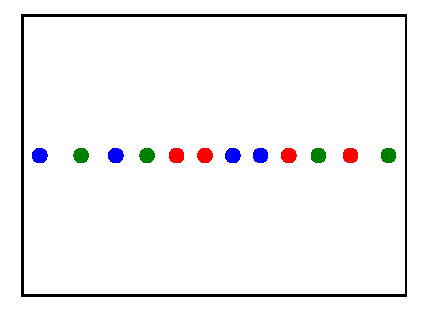
\includegraphics[width=4cm]{Figures/TSNE/DEMO/iteration_4.pdf}};
        
        % Add arrows between the figures
        \draw[->, thick] (input.east) -- (output.west) node[midway, above] {t-SNE};
    \end{tikzpicture}
    \caption{2D data point transformed into 1D data point using t-SNE}
    \label{fig:tsne_diagram}
\end{figure}

In order to calculate the t-SNE for a set of data points, we first need to calculate the conditional probability.
This is calculated based on the Equation \ref{eq:pij} below.
The author of t-SNE Van der Mateen \cite{tsne2} states:
“The similarity of datapoint $x_j$ to datapoint $x_i$ is the conditional probability, $p_{ij}$, that $x_i$ would pick $x_j$ as its neighbor if neighbors were picked in proportion to their probability density under a Gaussian centered at $x_i$.” 

\begin{equation}
\label{eq:pij}
p_{ij} = \frac{\exp(-\lVert x_i - x_j \rVert^2/2\sigma_i^2)}{\sum_{k \neq l} \exp(-\lVert x_k - x_l \rVert^2/2\sigma_i^2)} \
\end{equation}

In Equation \ref{eq:pij} $x_i$ and $x_j$ are two data points and $|x_i - x_j|$ is the Euclidean distance between the two.
The nominator in Equation \ref{eq:pij} is equal to the similarity between two points normalized by the variance $2\sigma_i^2$.
The whole expression is run through $exp()$ function to ensure the value stays positive and within boundaries.
The denominator in Equation \ref{eq:pij} serves as a normalisation factor, to ensure that the sum of probabilities for data point $x_i$ will sum to 1.

The $\sigma_i$ is also known as Gaussian bandwidth, Gaussian kernel or just variance is picked for each data point based on the number of neighbors in its vicinity.
In areas where data points are more crowded, $\sigma_i$ is usually smaller than in less crowded areas.
It is pre-calculated for every point using binary search. 
A search is complete when $\sigma_i$ outputs probability distribution $P_i$ that matches user-defined perplexity $Perp(P_i)$.

$$Perp(P_i) = 2^{H(P_i)}$$

Here, $H(P_i)$ is the entropy of the conditional probability distribution $P_i$.
The entropy of conditional probability distribution is a measure of perplexity.
Perplexity is one of the parameters defined by the user, and it's used as a measure of the number of effective neighbors, between which we will compute similarities.
High perplexity means that the distribution of the Gaussian kernel will be wide and contain more data points between which similarity will be computed.
Low perplexity means that the kernel will be narrow, so fewer data points will fit into it and therefore fewer data points will be compared.

The output of the algorithm is a map of every data point $y_i$.
These points are low dimensional counterparts of $x_i$.
Usually, these data points contain a comprehensible number of dimensions where $y_i \in \mathbb{R}^2$ or $\mathbb{R}^3$. 
Similarly, as in equation \ref{eq:pij} we can now use low dimensional data points $y_i$ and $y_j$ to calculate probability $q_{ij}$ in equation \ref{eq:gij}.
Here, t-student distribution with one degree of freedom is utilized to calculate the similarities.

\begin{equation}
\label{eq:gij}
q_{ij} = \frac{(1+\lVert y_i - y_j \rVert^2)^{-1}}{\sum_{k \neq l} (1+\lVert y_k - y_l \rVert^2)^{-1}} 
\end{equation}

$q_{ij}$ is again a conditional probability of finding $y_i$ and $y_j$ near each other but for fewer dimensions.

Setting up a cost function, which tries to minimize the difference between $q_{ij}$ and $p_{ij}$ should result in a low dimensional map where similar points should be near eachother.
The cost function is also known as Kullback-Leibler divergence seen in Equation \ref{eq:Klle}. 
The equation is the sum of all pairwise similarities between low and high-dimensional data points.
The smaller the $C$ the closer the similar data points are in low dimensional space.

\begin{equation}
\label{eq:Klle}
 C = \sum_{i \neq j}^n p_{ij} \log \frac{p_{ij}}{q_{ij}}
\end{equation}

The similarity is achieved over many iterations where we use gradient descent to minimize the Kullback-Leibler divergence seen in Equation \ref{eq:Klle}. 
The process can be seen in Figure \ref{fig:tsne_iterations_arrows}.

\begin{figure}[H]
    \centering
    \begin{tikzpicture} 
        % Draw the first subfigure
        \node (tsne1) at (0,0) {\includegraphics[width=0.25\textwidth]{Figures/TSNE/DEMO/iteration_1.pdf}};
        \node[above] at (tsne1.north) {0 iters};
        
        % Draw the second subfigure
        \node (tsne2) at (0.35\textwidth,0) {\includegraphics[width=0.25\textwidth]{Figures/TSNE/DEMO/iteration_2.pdf}};
        \node[above] at (tsne2.north) {150 iters};
        
        % Draw the third subfigure
        \node (tsne3) at (0.7\textwidth,0) {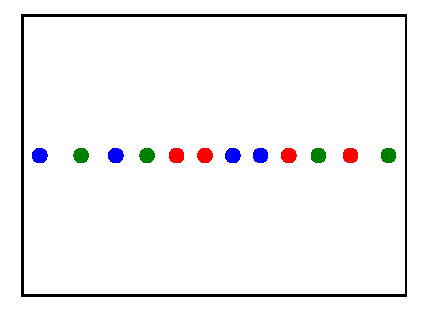
\includegraphics[width=0.25\textwidth]{Figures/TSNE/DEMO/iteration_4.pdf}};
        \node[above] at (tsne3.north) {400 iters};
        
        % Add arrows between the subfigures
        \draw[->, thick] (tsne1.east) -- (tsne2.west);
        \draw[->, thick] (tsne2.east) -- (tsne3.west);
    \end{tikzpicture}
    \caption{Iterations of t-SNE}
	\par
    \par\footnotesize{The input data can be seen in \ref{fig:tsne_diagram} }
	\label{fig:tsne_iterations_arrows}
\end{figure}


In our case, two dimensions will be used. Since this is a non-linear dimensionality reduction,
the axis usually presents dimensions that are hard to comprehend by the brain. 
It is important to keep in mind that the resulting low-dimensional representation is not necessarily interpretable in the same way as the original high-dimensional data.
This also means that the axes labels on the graphical presentations are meaningless.
In our case, we labeled the two axes as $dimension-1$ and $dimension-2$.

\section{Results}

The results will be presented in three subsections

\begin{itemize}
	\item Per-building LP
	\item Per-appliance LP
	\item Per-building per-appliance LP
\end{itemize}

%Most of the focus will be done on the per-appliance LP since it is the most universal.

The following figures are best viewed in color and a digital format. 
In the analysis, the reader can use the first figures to identify buildings and the second to identify the patterns and actual LPs.
Readers reading the digital version should have the ability to zoom into each cluster and see the actual samples. 
Readers reading a paper version can still explore the high-resolution figures online via the provided link below every figure.

\subsection{Results for Per-Building LPs}
%TODO
\label{ssec:res_pb_lp}
This LP is useful when it comes to comparing how 
activation patterns change over buildings and datasets.
Per-building data uses combined activations of all appliances to present 
the aggregated usage pattern.  

This section will first address non-normalized LPs and later move on to normalized LPs.
We have already addressed the methodology on normalization in Section \ref{ssec:norm}.
By normalizing the data we are essentially removing information from the LP.
This information contains knowledge of the number of the appliances in building and their usage intensity.
Knowing the two could be useful in scenarios where we are analyzing the magnitude of usage and not the patterns themselves.

Figure \ref{fig:tsne_scatter_non_norm_all} is using non-normalized data, meaning
the number of appliances in a building will affect the end LP.
The algorithm could pick up on how many and how much appliances are being used.
In some cases, such as energy poverty detection, this information is useful, as we are searching for buildings that exhibit reduced activation patterns.

\begin{figure}[H]
	\centering
	\caption{Projection of per-building LPs}
	\includegraphics[]{Figures/TSNE/TSNE_per_building/scatter_per_building.pdf}
	\label{fig:tsne_scatter_non_norm_all}
	\par
	\par\footnotesize{Full resolution figure: \url{https://github.com/jenkoj/msc/tree/main/Figures/TSNE/TSNE_per_building/scatter_per_building.pdf}}
\end{figure}

\begin{figure}[H]
	\centering
	\caption{Projection of per-building LPs with actual samples}
	\includegraphics[width=.9\textwidth]{Figures/TSNE/TSNE_per_building/img_scatter_per_building.png}
	\label{fig:tsne_pb_img_scatter_allall}
	\par
	\par\footnotesize{Full resolution figure: \url{https://github.com/jenkoj/msc/tree/main/Figures/TSNE/TSNE_per_building/img_scatter_per_building.png}}
\end{figure}


Figure \ref{fig:tsne_pb_img_scatter_allall} displays the LP for each sample. 
T-SNE provides an intuition of how LPs are connected in higher-dimensional space, and through analysis, we can find clusters with similar usage patterns.
Figure \ref{fig:tsne_pb_img_scatter_allall} shows that the left side has mostly samples with little activity, and the right side has more activity.
When looking at Figure \ref{fig:tsne_scatter_non_norm_all}, we can observe a clear pink colored cluster of LPs from UKDALE 1 and UKDALE 2, which contain plenty of appliances and may explain why they have many activators.
Some less obvious clusters formed in the bottom section for REFIT buildings 2, 3, 5, 6, 4 and 8. 

There are no recognizable patterns in the central part of the plot. 
Since there are no patterns, such LPs do not form clusters. 
The reason behind non-recognizable patterns is possibly because appliances like fridges contributed the majority of activations, which are not affected by the dweller, leading to random activations.
Similarly, there are no clusters in the far-left part of the plot because those profiles lack enough information to distinguish them. 

Even though the activations of LPs contained non-normalized activations, some clusters of buildings are quite close to each other.
Here we have to keep in mind the fact that through current presentations we can only observe usage patterns and not usage intensity, which was used as an input to t-SNE
This implies that these buildings have similar usage intensities but not necessarily usage patterns.
We can confirm this, by looking at Figure \ref{fig:tsne_pb_img_scatter_allall}, where it is hard to find what similarities between buildings and clusters that are close together.


% TODO you can write about activation intensify scaler. Max abs is note useful, since most of them would be dark
% We would need some kind of lgaritmic scaling, otherwirse buildings with little appliances would be completley dark and buildings with many appliances completly brihht.
% Either way, presenting these LPs is a hard task

%Efficiently presenting activation intensity is a hard task.
%if we would simply scale all LPs using max-abs scaler, we would be left with some LPs being completely dark and onthers completely white.
%To fix this issue we would have to introduce some kind of logarithmic scaling 

\subsubsection{Normalized LPs}

The issue mentioned in the previous Subsection \ref{ssec:res_pb_lp} can be addressed by normalizing the data between 0 and 1 as mentioned in methodology Section \ref{ssec:norm}.
The normalization should enable t-SNE to focus on finding similarities between the usage patterns.

Figure \ref{fig:tsne_pb_scatter_all_all} illustrates how normalization affects the algorithm.
By comparing Figures \ref{fig:tsne_scatter_non_norm_all} and \ref{fig:tsne_pb_scatter_all_all}, we can observe that the samples in the latter are much closer to each other, while still retaining the individual clusters.
This outcome is expected because normalization removes information regarding the number of appliances in the building.
With a reduced amount of information, LPs become more similar, and therefore clusters are closer together.

\begin{figure}[H]
	\centering
	\caption{Projection of normalized per-building LPs}
	\includegraphics[]{Figures/TSNE/TSNE_per_building/scatter_per_building_norm.pdf}
	\label{fig:tsne_pb_scatter_all_all}
	\par
	\par\footnotesize{Full resolution figure: \url{https://github.com/jenkoj/msc/tree/main/Figures/TSNE/TSNE_per_building/scatter_per_building_norm.pdf}}
\end{figure}

When observing the LPs in Figure \ref{fig:tsne_pb_img_norm_scatter_allall}, we can confirm that similar clusters are closer together.
In this case, the input of the algorithm was the same as our perception of the LPs.
Upon closer look, we can see a gradual and smooth change in patterns as we move across the plot.
If we recall from before that was not the case in Figure \ref{fig:tsne_pb_img_scatter_allall} where we were analyzing non-normalized LPs.
This observation is important, as it is visual proof, that normalization did help the t-SNE to focus on the usage patterns.
% Figure \ref{fig:tsne_pb_img_norm_scatter_allall} presents only the main cluster of samples.
% Since the smaller cluster presents mostly low entropy data, it was cut out. 
% If the reader wants to see the samples in the cluster, the very same cluster can be found on the far left in Figure \ref{fig:tsne_pb_img_scatter_allall}.

\begin{figure}[H]
	\centering
	\caption{Projection of normalized per-building LPs with actual samples}
	\includegraphics[width=.9\textwidth]{Figures/TSNE/TSNE_per_building/img_scatter_per_building_norm.png}
	\label{fig:tsne_pb_img_norm_scatter_allall}
	\par
	\par\footnotesize{Full resolution figure: \url{https://github.com/jenkoj/msc/tree/main/Figures/TSNE/TSNE_per_building/img_scatter_per_building_norm.png}}
\end{figure}

Upon closer inspection of Figure \ref{fig:tsne_pb_img_norm_scatter_allall} we can see that the general pattern is that there is less activity during the night with one peak in the morning and evening hours.
Some buildings are more active during the week and again some more during the weekend.
A lot of the data is from UK-DALE 1 colored pink. 
It is possible to see that the building has one big cluster where activations are generally similar, with few outliers, where the pattern completely changed. 
This happens due to events such as vacations, holidays or weather-induced behavioral changes.

The key difference between non-normalized and normalized LPs is that,
non-normalized LPs enable t-SNE to identify similarities in the number of appliances and their usage intensity,
while normalized LPs force t-SNE to focus on similarities in the actual usage pattern.
Normalized LPs provide information about when appliances are likely to be used throughout the day, while non-normalized LPs provide insight into the magnitude of appliance usage.

Based on the above observations, we could say that usage patterns are more similar than the number of activations across buildings.

\subsubsection{Euclidian distance of samples for every building}
\label{ssec:tsne_euclidian_distance}

A significant observation is that LPs closer together have more similar consumption throughout every month.
By measuring the distance between LPs of the same building we can estimate the strength of the household's routine. 
Figure \ref{fig:tsne_euclidian} presents the Euclidean distance between samples for a given building.
The larger the value, the longer the distance and the less similar the consumption trough every month is.

\begin{figure}[H]
	\centering
	\caption{Euclidean distance of samples for every building on normalized LPs}
	\includegraphics[]{Figures/EC/CORR_TSNE/tnse_euclidian.pdf}
	\label{fig:tsne_euclidian}
\end{figure}

The methodology and the equation for calculating Euclidian distance were thoroughly discussed in section \ref{ssec:lp_similarity}.
Since t-SNE uses Euclidean distance at its base, we essentially measured the values of the last t-SNE iteration.

As we will use the Euclidean distance plot in the next Chapter \ref{chapter6} as a comparison, we have used only samples from the REFIT dataset.
A more detailed analysis will follow in this chapter as well.
As for now, we can see that the buildings with the most similar consumption pattern are 5 and 13. 
They both lay on the right side of the plot and have a similar activation pattern, with very few activations throughout the weekday.
This could point toward the fact that people with steady jobs have very steady consumption patterns.

\subsection{Per-Appliance}

We can use per-appliance LPs to examine how different appliances 
are used in a single building, how a single appliance is being used across other buildings or how many appliances are being used in many buildings.
Per appliance LPs are built using sub-meter data, meaning each LP should present each appliance.

\subsubsection{Single Appliance Over Many Buildings}

Using one appliance and the building as a label,
allows us to examine how the same type of appliance is being used across different buildings.

Fridges are generally a bad indicator when it comes to user behavior since the user does not affect its operation. 
The only case when the user interacts with it is when opening the door and turning on the light inside. 
Usually, this event is dwarfed by the activations of a compressor. 
This also means that the usage pattern should be the same across all buildings. 
This can be seen in Figure \ref{fig:tsne_pa_scatter_all_fridge}, 
where apart from REFIT buildings 1 and 11, there are no clusters.


\begin{figure}[H]
	\centering
	\caption{Projection of fridge LPs for various buildings}
	\includegraphics[]{Figures/TSNE/TSNE_per_appliance/scatter_refit_fridge_freeezer_fridge_freezer.pdf}
	\label{fig:tsne_pa_scatter_all_fridge}
	\par
	\par\footnotesize{Full resolution figure: \url{https://github.com/jenkoj/msc/tree/main/Figures/TSNE/TSNE_per_appliance/scatter_refit_fridge_freeezer_fridge_freezer.pdf}}
\end{figure}

Figure \ref{fig:tsne_pa_img_scatter_all_fridge} Shows mostly bright images, apart from a few outliers.
LPs scattered in a circle are generally less dynamic than the ones at the bottom.
Figure \ref{fig:tsne_pa_img_scatter_all_fridge} is a good example of how LPs with little to no human interaction, can look a lot different. 
This could be due to different makes of the appliances, malfunctions of the appliance or the meter measuring it.

\begin{figure}[H]
	\centering
	\caption{Projection of fridge LPs for various buildings with actual samples}
	\includegraphics[width=.9\textwidth]{Figures/TSNE/TSNE_per_appliance/img_scatter_refit_fridge_freeezer_fridge_freezer.png}
	\label{fig:tsne_pa_img_scatter_all_fridge}
	\par
	\par\footnotesize{Full resolution figure: \url{https://github.com/jenkoj/msc/tree/main/Figures/TSNE/TSNE_per_appliance/img_scatter_refit_fridge_freeezer_fridge_freezer.png}}
\end{figure}

Figure \ref{fig:tsne_pa_scatter_all_kettle} shows how,
compared to fridges, kettles have many clear clusters that are spaced out between each other. 
This could mean that every household uses a kettle a bit differently.
These clusters are a good example where we can observe how strong is a routine of a user.
The closer together the samples in individual clusters are, the higher the routine since samples are more similar to each other.

\begin{figure}[H]
	\centering
	\caption{Projection of kettle LPs for various buildings}
	\includegraphics[]{Figures/TSNE/TSNE_per_appliance/scatter_refit_kettle.pdf}
	\label{fig:tsne_pa_scatter_all_kettle}
	\par
	\par\footnotesize{Full resolution figure: \url{https://github.com/jenkoj/msc/tree/main/Figures/TSNE/TSNE_per_appliance/scatter_refit_kettle.pdf}}
\end{figure}

Figure \ref{fig:tsne_pa_img_scatter_all_kettle} shows us that images on the lower part 
of the plot contain less activity than the others. 
LPs that are closer together have more similar activation patterns.
Similar activation patterns are caused by similar behavior, which is essentially a routine.
This means that this projection could be used to calculate how much a behavior variates in time for each building.
This could be calculated by measuring the scattering of samples (variance) for each building.

If we find samples that always activate in the same morning buckets, we would see that they form a straight line on the y-axis.
This is the daily routine. One such example can be seen in Figure \ref{fig:tsne_pa_scatter_all_kettle} in cluster REFIT 5 and REFIT 9, where we can see the lines and the pattern throughout the day. 
Since the routine is present, the samples look more similar and are therefore closer together. 
This does not necessarily mean that the closer the samples higher the routine.
They could also be together in case of "ordered chaos" such as can be seen in Figure \ref{fig:tsne_pa_scatter_all_kettle} for building refit 16 and refit 8 where there is no pattern through the day.
So the scattering is not a precise metric when it comes to the routine, but it gives us a rough idea of its presence.
As mentioned earlier in this chapter the strength of a routine is an important feature that will be used
in Chapter \ref{chapter6}, where we will build an elderly care anomaly detection system.

\begin{figure}[H]
	\centering
	\caption{Projection of kettle LPs for various buildings with actual samples}
	\includegraphics[width=.9\textwidth]{Figures/TSNE/TSNE_per_appliance/img_scatter_refit_kettle.png}
	\label{fig:tsne_pa_img_scatter_all_kettle}
	\par
	\par\footnotesize{Full resolution figure: \url{https://github.com/jenkoj/msc/tree/main/Figures/TSNE/TSNE_per_appliance/img_scatter_refit_kettle.png}}
\end{figure}

% Figure \ref{fig:tsne_pa_scatter_all_microwave} shows that microwaves are again a bit different from the kettle.
% They are more clustered than the fridges, and less than the kettles, even though they are used similarly.
% This could be due to additional electronics such as a clock that are built into
% the appliance. This could lead to some samples being registered as turned on due to 
% a "dark" current. One other difference between the two is that microwave has more than one mode of operation.

% \begin{figure}[H]
% 	\centering
% 	\caption{Projection of microwave LPs for various buildings}
% 	\includegraphics[width=1.2\textwidth]{Figures/TSNE/TSNE_per_appliance/all/scatter_all_microwave.png}
% 	\label{fig:tsne_pa_scatter_all_microwave}
% \end{figure}

% Figure \ref{fig:tsne_pa_img_scatter_all_microwave} shows the faulty samples could be the ones in the upper left part of the plot since they are too bright.
% They do present a pattern, but it is questionable what it presents since it seems like it's turned on during the nighttime. 
% Images at the other end show less lot less activity, which could indicate that
% the household does not use microwaves as much. The most interesting LPs are in the middle of the 
% plot, where it is possible to observe clear activation patterns. 

% \begin{figure}[H]
% 	\centering
% 	\caption{Projection of microwave LPs for various buildings with actual samples}
% 	\includegraphics[width=.9\textwidth]{Figures/TSNE/TSNE_per_appliance/all/img_scatter_allmicrowave.png}
% 	\label{fig:tsne_pa_img_scatter_all_microwave}
% \end{figure}

The last per-appliance example is television presented in Figure \ref{fig:tsne_pa_scatter_all_tv}. 
Television was chosen since it is the most commonly occurring appliance.
Interestingly enough, televisions form nice clusters with a few outliers.
Clusters are separated but close together, this could mean that usage patterns across buildings are unique
but not that different from one another. 
The LPs in some clusters are also close to each other, which could also indicate 
a higher routine.

\begin{figure}[H]
	\centering
	\caption{Projection of TV LPs for various buildings}
	\includegraphics[]{Figures/TSNE/TSNE_per_appliance/scatter_refit_television.pdf}
	\label{fig:tsne_pa_scatter_all_tv}
	\par
	\par\footnotesize{Full resolution figure: \url{https://github.com/jenkoj/msc/tree/main/Figures/TSNE/TSNE_per_appliance/scatter_refit_television.pdf}}
\end{figure}

The images in Figure \ref{fig:tsne_pa_img_scatter_all_tv} prove the fact that outliers' consumption is a lot different.
Again the bright images could be the results of faulty appliances, faulty meters or simply odd behavior.
Figure \ref{fig:tsne_pa_img_scatter_all_tv} also enables us to see that TVs are primarily used 
in the evening hours. Outliers from the main cluster show slightly different behavior. One such 
example is the blue cluster (building REFIT 4), where appliances are mostly used in the morning hours. 
One other interesting observation can be made when looking at the purple cluster. This is the far low cluster for building REFIT 8.
Here, the TV is being consistently used every day in the early morning hours.
This is portrayed as a straight line.
There could be two possible explanations for this.
First is simply a high routine of a user, who turns on the TV every morning to listen to the news.
The other is that the TV updates itself every morning. This is probably not the case since updates do not occur on regular basis.
What is also interesting, is that the very same pattern can be observed in a few other buildings, one example being building REFIT 19.

\begin{figure}[H]
	\centering
	\caption{Projection of TV LPs for various buildings with actual samples.}
	\includegraphics[width=.9\textwidth]{Figures/TSNE/TSNE_per_appliance/img_scatter_refit_television.png}
	\label{fig:tsne_pa_img_scatter_all_tv}
	\par
	\par\footnotesize{Full resolution figure: \url{https://github.com/jenkoj/msc/tree/main/Figures/TSNE/TSNE_per_appliance/img_scatter_refit_television.png}}
\end{figure}

\subsubsection{Per-Appliance LPs - Comparing Appliances}

% Figure \ref{fig:tsne_papb_scatter_all} presents the general picture of where each appliance lays in comparison to the other.
% One obvious issue here is that there are too many appliances, and it is impossible to comprehend the plot.

% \begin{figure}[H]
% 	\centering
% 	\caption{Projection of per-appliance LPs}
% 	\includegraphics[width=1.2\textwidth]{Figures/TSNE/TSNE_results/all/scatter_all_all_lgimgs.png}
% 	\label{fig:tsne_papb_scatter_all}
% \end{figure}

% The same goes for image presentation in Figure \ref{fig:tsne_papb_img_scatter_all}. 
% We can see, that most active appliances are the ones in the bottom left,
% by moving to the upper right part of the corner, we can see less activity.
% Less activity does not necessarily mean that LPs contain less information about user behavior.

% \begin{figure}[H]
% 	\centering
% 	\caption{Projection of per-appliance LPs with actual samples}
% 	\includegraphics[width=.9\textwidth]{Figures/TSNE/TSNE_results/all/img_scatter_allall_lgimgs.png}
% 	\label{fig:tsne_papb_img_scatter_all}
% \end{figure}

To get a general idea of where each appliance group lies,
let's filter out all appliances that have less than 150 samples.
Applying this filter yields Figure \ref{fig:tsne_papb_scatter_all_reduced}.

\begin{figure}[H]
	\centering
	\caption{Projection of filtered per-appliance LPs}
	\includegraphics[]{Figures/TSNE/TSNE_PHPA/phpa_reduced_15.pdf}
	\label{fig:tsne_papb_scatter_all_reduced}
	\par
	\par\footnotesize{Full resolution figure: \url{https://github.com/jenkoj/msc/tree/main/Figures/TSNE/TSNE_PHPA/phpa_reduced_15.pdf}}
\end{figure}

Figure \ref{fig:tsne_papb_scatter_all_reduced} shows how these 10 appliances are connected in high dimensional space.
Kettles, microwaves and toasters are quite similar when it comes to usage patterns.
They are operated for a short amount of time and are usually used in users' routines in the morning or evening.
These appliances are located in the upper left part of the plot.

The second group of appliances that are quite near each other is white
goods (without fridges) such as washing machines, dishwashers, dryers etc.
Let's say that they are white goods with a program. 
This group of appliances is located in the upper right part of the plot.

The third group of appliances is white goods with a compressor.
They are usually not affected by human interaction and are therefore harder to cluster.
They are located in the lower part of the plot.

The final group of appliances is televisions and computers. They lie 
on a bridge between the fridges and other groups. 

% \begin{figure}[H]
% 	\centering
% 	\caption{Projection of filtered per-appliance LPs with actual samples}
% 	\includegraphics[width=.9\textwidth]{Figures/TSNE/TSNE_results/all/img_scatter_allall_reduced_max.png}
% 	\label{fig:tsne_papb_img_scatter_all_reduced}
% \end{figure}

% Even though the set of LPs is different due to filtering,
% the Figure \ref{fig:tsne_papb_img_scatter_all_reduced},
% retains a similar structure to the previous Figure \ref{fig:tsne_papb_scatter_all_reduced}. 

Knowing that a pattern exists, we can use the newly found group to define new appliance groups.
The following 8 groups will be defined
\begin{itemize}
    \item Kitchen appliances - toasters, ovens, microwaves, etc.
    \item Fridges and freezers  - contains fridges, freezers and fridge freezers or white goods with a compressor
    \item White goods - washers, dryers, dishwashers i.e. white goods with a program
    \item heating and cooling - Electric radiators, dehumidifiers and HVACs
    \item leisure -  Living room appliances such as TVs, games consoles, audio amps, HTPCs, etc.
    \item home office - Computer, laptops, printers, network equipment, chargers, etc.
    \item lightning - lights and lamps
    \item Others - unknown and unlabeled appliances
\end{itemize}

Applying these groups yields Figure \ref{fig:tsne_papb_scatter_all_groups}.
The new plot shows how, although appliances could be used by a different
user, maybe even by users in a different part of the EU or world,
they can be grouped in a high-dimensional space. 

\begin{figure}[H]
	\centering
	\caption{Projection of grouped per-appliance LPs}
	\includegraphics[]{Figures/TSNE/TSNE_PHPA/phpa_grouped_15.pdf}
	\label{fig:tsne_papb_scatter_all_groups}
	\par
	\par\footnotesize{Full resolution figure: \url{https://github.com/jenkoj/msc/tree/main/Figures/TSNE/TSNE_PHPA/phpa_grouped_15.pdf}}
\end{figure} 

The Figure \ref{fig:tsne_papb_img_scatter_all_groups} below is the same as the first Figure \ref{fig:tsne_papb_img_scatter_all} in the subsection,
except it is easier to use color to see the appliance they present

\begin{figure}[H]  
	\centering
	\caption{Projection of grouped per-appliance LPs with actual samples}
	\includegraphics[width=1.1\textwidth]{Figures/TSNE/TSNE_PHPA/img_scatter_all_all_groups.png}
	\label{fig:tsne_papb_img_scatter_all_groups}
	\par
	\par\footnotesize{Full resolution figure: \url{https://github.com/jenkoj/msc/tree/main/Figures/TSNE/TSNE_PHPA/img_scatter_all_all_groups.png}}
\end{figure}

To better emphasize the details from Figure \ref{fig:tsne_papb_img_scatter_all_groups} and \ref{fig:tsne_papb_scatter_all_groups} we present zoomed-in areas of key locations with Figure \ref{fig:t-sne_zoomed}.
\begin{figure}[H] 
	\centering
	\caption{Projection of grouped per-appliance LPs with actual samples}
	\includegraphics[width=1\textwidth]{Figures/TSNE/TSNE_PHPA/t-sne_zoomed.png}
	\label{fig:t-sne_zoomed}
	\par
	\par\footnotesize{Full resolution figure: \url{https://github.com/jenkoj/msc/tree/main/Figures/TSNE/TSNE_PHPA/t-sne_zoomed.png}}
\end{figure}

% One issue that causes the t-SNE algorithm an issue is low entropy data or 
% in other words, images that are almost completely dark or white, due to various faults in appliances or measurements.

% If we calculate the entropy for each image and set a threshold, it is possible to filter out these samples. 
% By setting an entropy threshold of 0.5, we filter out around 5 \% of all samples. 

% \begin{figure}[H]
% 	\centering
% 	\caption{Projection of entropy filtered per-appliance LPs}
% 	\includegraphics[width=.8\textwidth]{Figures/TSNE/TSNE_results_entropy/all/scatter_all_all.png}
% 	\label{fig:tsne_papb_scatter_ent_all_groups}
% \end{figure}

% Again, we can apply appliance grouping and get nicely formed clusters, such as can be seen in Figure \ref{fig:tsne_papb_img_scatter_ent_all_groups}.

% \begin{figure}[H]
% 	\centering
% 	\caption{Projection of entropy filtered per-appliance LPs with actual samples}
% 	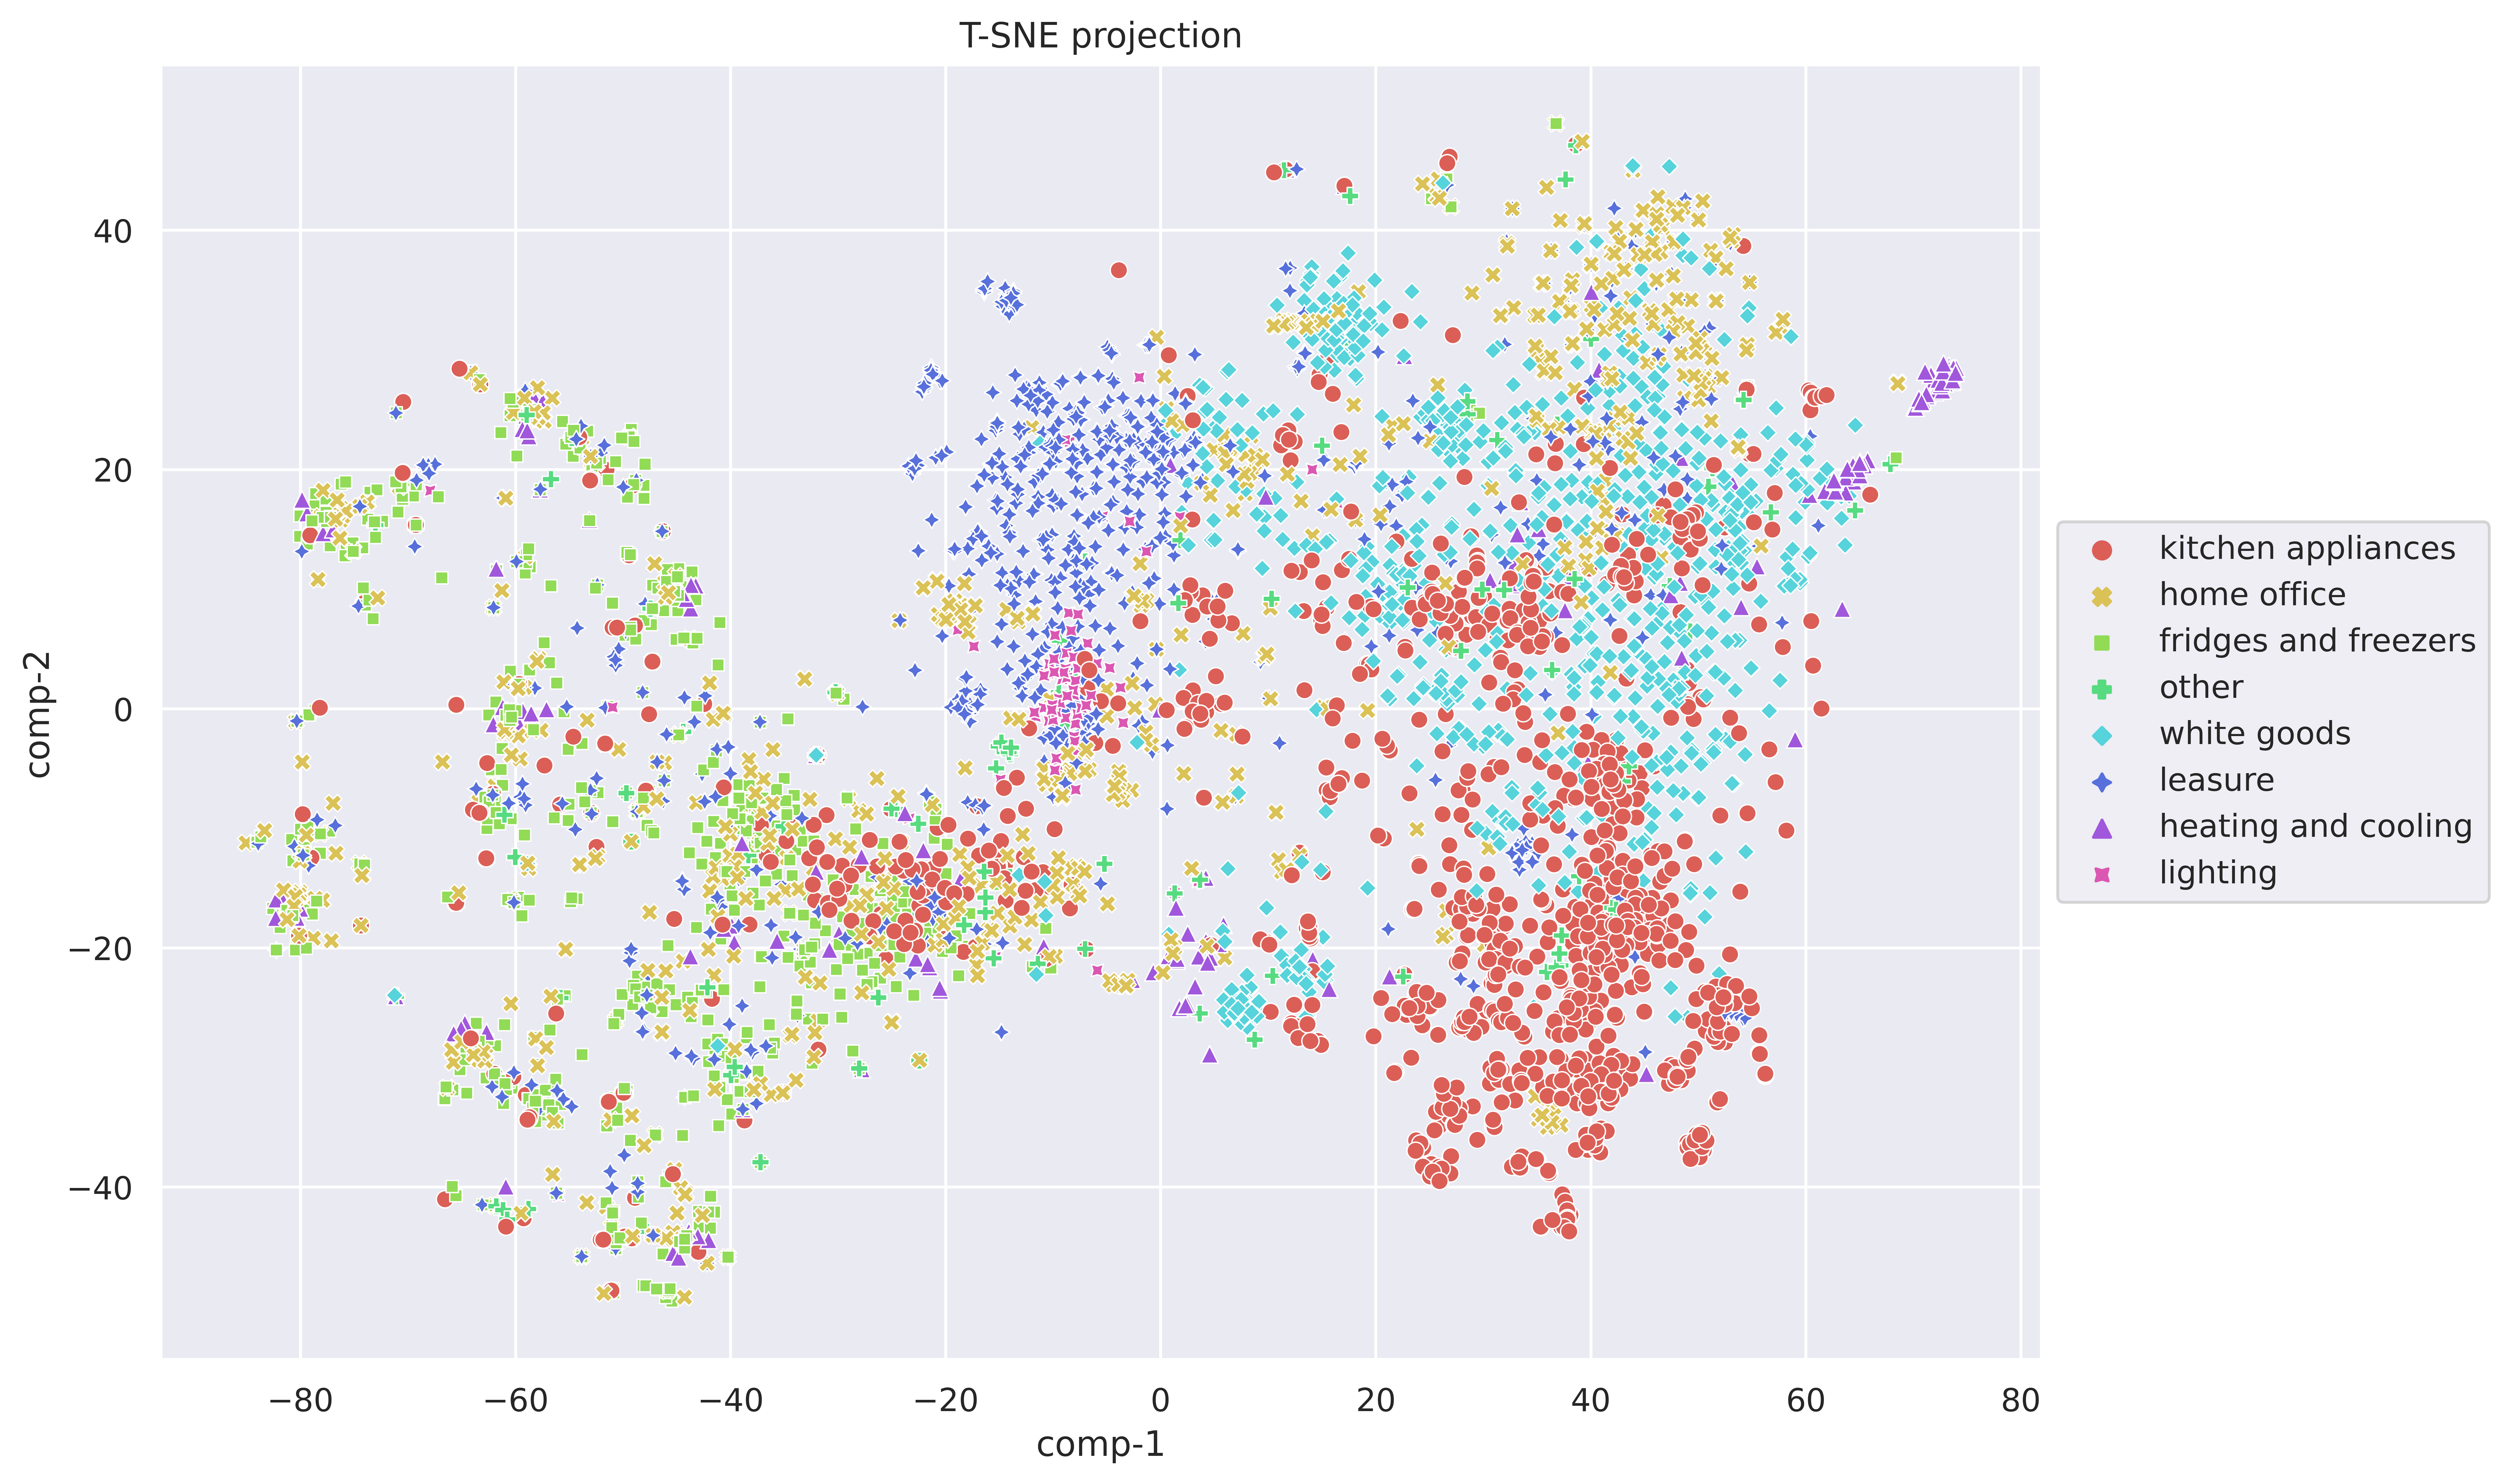
\includegraphics[width=.8\textwidth]{Figures/TSNE/TSNE_results_entropy/all/scatter_all_all_groups.png}
% 	\label{fig:tsne_papb_img_scatter_ent_all_groups}
% \end{figure}


% \subsubsection{Comparing Appliances in a Building}

% It is also possible to use per-appliance data to study
% individual buildings, and how each appliance is used.
% In this case, we have used building 8 from REFIT as an example.

% \begin{figure}[H]
% 	\centering
% 	\caption{Projection of per-appliance LPs in a single building}
% 	\includegraphics[width=.8\textwidth]{Figures/TSNE/TSNE_results/refit/scatter_refit_8.png}
% 	\label{fig:tsne_papb_scatter_ent_refit8}
% \end{figure}

% In general, the scattering is similar to before.
% Fridges and freezers are located opposite of white goods and kitchen appliances. 
% The television lies somewhere in between. 

% \begin{figure}[H]
% 	\centering
% 	\caption{Projection of per-appliance LPs in a single building with actual samples}
% 	\includegraphics[width=.9\textwidth]{Figures/TSNE/TSNE_results/refit/img_scatter_refit8.png}
% 	\label{fig:tsne_papb_img_scatter_ent_refit8}
% \end{figure}

% Similar to before Figure \ref{fig:tsne_papb_img_scatter_ent_refit8} shows the fridge cluster as the most active,
% with the least interesting information. In the middle, we can again observe the TV that is mostly being used
% in the evening hours. The samples also point to the possibility of a high-user routine in the early morning hours.
% The high routine is portrayed as a straight line on the figures. 

% In this case, when observing white goods in pink and purple boxes, it is possible to see that this user primarily uses them during the night hours.
% This could point out that the user is making use of cheaper tariffs.

% One other interesting observation that can be made here is comparing kettles, microwaves and toasters.
% Usually, these appliances are used similarly and in similar parts of the day. 
% Here the toaster and microwave are being used periodically, but the kettle is being used throughout the day with no general pattern.
% It is self-obvious that some users have higher routines than others, but this observation
% would add that some users can have a higher routine for some appliances and lower for others, of the same type. 

\subsection{Per-Appliance Per-Building}

To study the usage by comparing all appliances between buildings,
we have to use one of the proposed LPs and in this case, this is a Bag of appliances.

\subsubsection{Bag of Appliances}

This LP is a combination of the LPs above,
except it offers a larger detail when observing groups of appliances.
Since we are using one dimension for appliances, we will use only the daily dimension.

To construct such a profile we need a universal way of constructing it.
This is done by measuring how many times each appliance occurs in the datasets,
then this list is sorted from most common to least common, and finally, the top 30 are selected.

The problem with such a comparison is, that it is best 
if all buildings would use the same appliances.
Since that is not the case, missing appliances are portrayed as always off. 

This is the main reason why we can see in Figure \ref{fig:tsne_boa_scatter_refit8} the clusters are separated quite a bit.
We can still see that some clusters are closer than others,
meaning they are more similar.  

\begin{figure}[H]
	\centering
	\caption{Projection of a bag of appliances LPs for various buildings}
	\includegraphics[]{Figures/TSNE/TSNE_BOA/scatter_refit_boa.pdf}
	\label{fig:tsne_boa_scatter_refit8}
	\par
	\par\footnotesize{Full resolution figure: \url{https://github.com/jenkoj/msc/tree/main/Figures/TSNE/TSNE_BOA/scatter_refit_boa.pdf}}
\end{figure} 

Figure \ref{fig:tsne_boa_img_scatter_refit8} shows that LPs are split 
between two poles. 
By observing the Figure it is possible to see that all the bottom clusters
have more than one active white good with a compressor (fridges and freezers), while
the top ones have only one. In general, the bottom buildings have more appliances,
with more activity than the top ones. 

\begin{figure}[H]
	\centering
	\caption{Projection of a bag of appliances LPs for various buildings with actual samples}
	\includegraphics[width=.9\textwidth]{Figures/TSNE/TSNE_BOA/img_scatter_boa.png}
	\label{fig:tsne_boa_img_scatter_refit8}
	\par
	\par\footnotesize{Full resolution figure: \url{https://github.com/jenkoj/msc/tree/main/Figures/TSNE/TSNE_BOA/img_scatter_boa.png}}
\end{figure}

\section{Discussion}

We used t-SNE to show how LPs are related in high-dimensional space, by mapping them into two-dimensional space.
We used three different types of LPs: per-building, per-building per-appliance, a bag of appliances, and per-appliance.
Per-building load profiles offered a look into how activations patterns differ across different buildings and datasets.
Per-building per-appliance bag of appliance load profiles offered the same thing, but in greater detail.
Per-appliance load profiles were the most versatile and were utilized in the most various ways:
First, we have shown how the same type of appliance is being used across various buildings.
Next, we compared appliances with each other. 
Since the plot was hard to comprehend, we have defined appliance groups.
These new groups formed clusters, which furthermore revealed the relation between LPs. 
Finally, we compared how appliance load profiles are connected in a single building. 

One of the main findings of this chapter was the formation of appliance groups.
Such groups enable us to look into the similarity of their activation profiles and enable us to understand which groups have similar usage patterns.
Another important piece of information these groups contain is the strength of the user's routine.
The closer the samples, the more similar their activation is, which means the user has a higher routine.
Such a routine will be useful in the next chapter, where we will try to evaluate if it is strong enough to detect anomalies.

\section{Summary}

The analysis provided a look into the relationships between LPs and their consumption patterns.
We were able to group appliances into categories and found a presence of routine in the LPs
These findings will be valuable in the next chapter where we continue to explore the potential applications of LPs.


% \chapter{Elderly Care Assisted Living System} % Main chapter title

\label{chapter6} % Change X to a consecutive number; for referencing this chapter elsewhere, use \ref{ChapterX}

%----------------------------------------------------------------------------------------
%	SECTION 1
%----------------------------------------------------------------------------------------

\section{Introduction}


Elderly care has been addressed by many EU-funded research projects since the aging population is one of the main issues facing the EU. 
There are many solutions to this problem.
One approach is invasive, such as the use of wearables, sound sensors, and IR occupancy detectors, among others.
This approach has been discussed in numerous publications.
Reviews \cite{elderReview1}, \cite{elderReview2}, and \cite{elderReview3} present and discuss this method.

Authors \cite{elderNILM} and \cite{elderNILMDementia} tried to solve this issue using a non-invasive approach with NILM algorithms. 
In the case of a non-invasive approach, no additional meters need to be installed, as per-appliance usage can be disaggregated.
While this is practical from the "no additional equipment needed" side, it is a bit less practical from the efficiency and accuracy side, especially for larger buildings. 

There is a middle ground between invasive and non-invasive approaches, as explored by the authors of papers \cite{elder1} and \cite{elder2}. 
It is possible to use sub-meters for each appliance and indirectly observe the usage pattern. 
The advantage of this approach is that the elder does not need to wear a device. 
The disadvantage is that new meters need to be installed for the most commonly used appliances. 
Our approach will use the latter.

\section{Goal}

The chapter will focus on building an elderly care system that will use users' periodic usage patterns to detect anomalies.
Anomalies could be anything from a fall, stroke, or altered usage pattern due to dementia. 
The algorithm will be designed based on the LP \ref{fig:PHPA}, which we discussed in Chapter \ref{chapter4}.
The figure shows that the first appliances used in the morning are a kettle and toaster, and with a delay of one hour, the microwave and TV. 
If none of these appliances are used within that hour, then that hour is considered anomalous.
This means that the algorithm will be able to detect an anomaly within 1 hour of its occurrence.

\section{Methodology}

\subsection{Defining an Anomaly}

Since the elderly care system is based on anomaly detection, we first have to define it.
In our case, an anomaly occurs when something that should operate, does not. 
Based on this definition, we will develop an anomaly detection algorithm. 

\subsection{Building Anomaly Detection Algorithm}

The following section presents the steps taken while designing this algorithm.

\subsubsection{Step One}
To detect the anomalies, one first needs to build a daily activation profile for each appliance, such as the one previously shown in Figure \ref{fig:PHPA}.
In this specific case, we will be using 2h buckets, yielding a total of 12 buckets. 

\subsubsection{Step Two}
The second step is to ignore appliances that are always on by calculating the standard deviation of activations for each bucket. 
The activations are normalized between 0 and 1. 
This step is important so that appliances that are always on, such as fridges or freezers, get ignored. 
These appliances are detected based on the width of their activation normal distribution. 
Periodic (on an hourly basis) appliances should have narrow distributions, and the more dynamic ones should have wider distributions.
This can be seen in examples from building 2.
\begin{figure}[H]
    \centering
    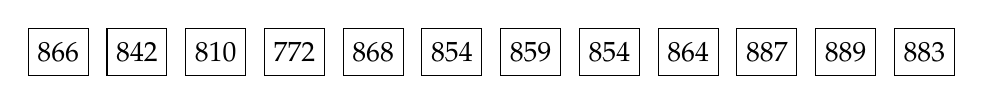
\begin{tikzpicture}
        \coordinate (s) at (0,0);
        \foreach \num in {866, 842, 810, 772, 868, 854, 859, 854, 864, 887, 889, 883}{
        \node[minimum size=6mm, draw, rectangle] at (s) {\num};
        \coordinate (s) at ($(s) + (1,0)$);
        }
    \end{tikzpicture}
    \caption{Daily activations for fridge $\sigma$ = 0.036}
    \label{arr:fridge_acts}
\end{figure}

\begin{figure}[H]
    \centering
    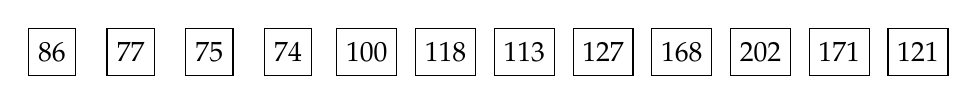
\begin{tikzpicture}
        \coordinate (s) at (0,0);
        \foreach \num in {86, 77, 75, 74, 100, 118, 113, 127, 168, 202, 171, 121}{
        \node[minimum size=6mm, draw, rectangle] at (s) {\num};
        \coordinate (s) at ($(s) + (1,0)$);
        }
    \end{tikzpicture}
    \caption{Daily activations for audio system $\sigma$ = 0.2}
    \label{arr:as_acts}
\end{figure}

\begin{figure}[H]
    \centering
    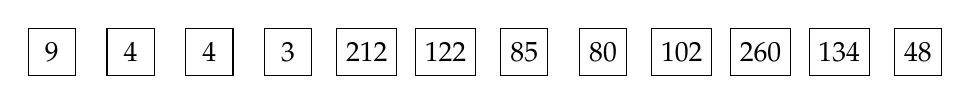
\begin{tikzpicture}
        \coordinate (s) at (0,0);
        \foreach \num in {9, 4, 4, 3, 212, 122, 85, 80, 102, 260, 134, 48}{
        \node[minimum size=6mm, draw, rectangle] at (s) {\num};
        \coordinate (s) at ($(s) + (1,0)$);
        }
    \end{tikzpicture}
    \caption{Daily activations for microwave $\sigma$ = 0.3}
    \label{arr:microwave_acts}
\end{figure}

Based on results from all appliances a threshold of $\sigma$ = 0.1 was set.
This method will also get rid of appliances that are always on due to their specific nature such as server computers 
or fridges. 

\subsubsection{Step Three}

Next, appliances that trigger together must be grouped. 
This means we must find parts of the day when they are operating together.
Due to the filtering in the previous step, we are left with appliances whose usage varies throughout the day. 
Some appliances are on even when the user is not necessarily using them, this can be seen in Figure \ref{arr:as_acts}.
One of many ways to do this grouping is to normalize the activations, which yields a metric that tells us the probability of that appliance being turned on compared to the rest of the day. 
If we apply this to the microwave and audio system appliances, the result is the following: 

\begin{figure}[H]
    \centering
    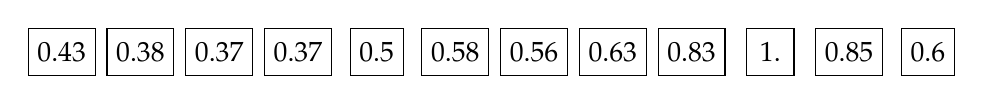
\begin{tikzpicture}
        \coordinate (s) at (0,0);
        \foreach \num in {0.43, 0.38, 0.37, 0.37, 0.5 , 0.58, 0.56, 0.63, 0.83, 1. , 0.85,
        0.6}{
        \node[minimum size=6mm, draw, rectangle] at (s) {\num};
        \coordinate (s) at ($(s) + (1,0)$);
        }
    \end{tikzpicture}
    \caption{Daily activations for audio system $\sigma$ = 0.2}
    \label{arr:as_acts_norm}
\end{figure}

\begin{figure}[H]
    \centering
    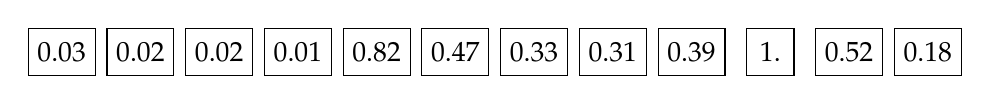
\begin{tikzpicture}
        \coordinate (s) at (0,0);
        \foreach \num in {0.03, 0.02, 0.02, 0.01, 0.82, 0.47, 0.33, 0.31, 0.39, 1.  , 0.52,
        0.18}{
        \node[minimum size=6mm, draw, rectangle] at (s) {\num};
        \coordinate (s) at ($(s) + (1,0)$);
        }
    \end{tikzpicture}
    \caption{Daily activations for microwave $\sigma$ = 0.3}
    \label{arr:microwave_acts_norm}
\end{figure}

Finally, a suitable threshold must be selected.
The threshold of 0.5 was selected, which yields the following vectors:

\begin{figure}[H]
    \centering
    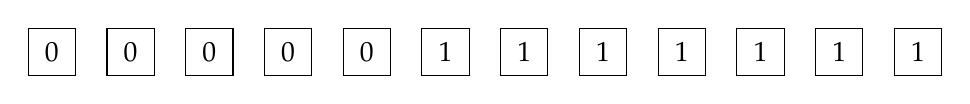
\begin{tikzpicture}
        \coordinate (s) at (0,0);
        \foreach \num in {0, 0, 0, 0, 0, 1, 1, 1, 1, 1, 1, 1}{
        \node[minimum size=6mm, draw, rectangle] at (s) {\num};
        \coordinate (s) at ($(s) + (1,0)$);
        }
    \end{tikzpicture}
    \caption{Daily activations for audio system}
    \label{arr:as_acts_vec}
\end{figure}

\begin{figure}[H]
    \centering
    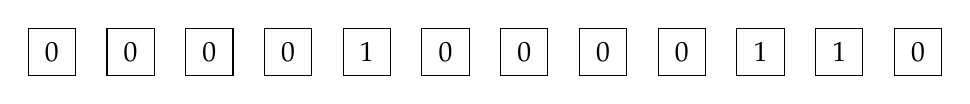
\begin{tikzpicture}
        \coordinate (s) at (0,0);
        \foreach \num in {0, 0, 0, 0, 1, 0, 0, 0, 0, 1, 1, 0}{
        \node[minimum size=6mm, draw, rectangle] at (s) {\num};
        \coordinate (s) at ($(s) + (1,0)$);
        }
    \end{tikzpicture}
    \caption{Daily activations for microwave with one usage peak in the morning and the other in the evening}
    \label{arr:microwave_acts_vec}
\end{figure}

The vectors show us that the microwave has two usage peaks, where the audio system can be used anytime throughout the day.
It is possible to do this for all appliances, which results in a 2D matrix. 
Using this matrix we can build rules for which appliances are being used together.
Figure \ref{arr:act_mat} uses rows for appliances and columns for buckets.  
If we use terminology from image processing the matrix \ref{arr:act_mat} is essentially a highly saturated LP \ref{fig:PHPA},
which can be easily processed by computer algorithms due to binary encoding. 

\begin{figure}[H]
    \centering
    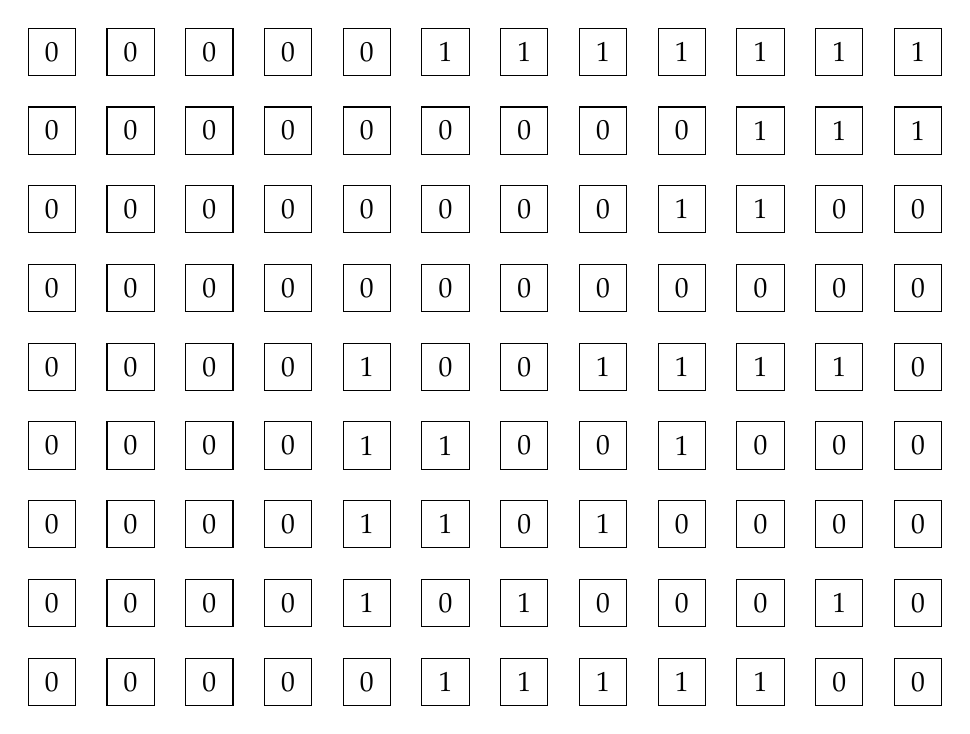
\begin{tikzpicture}
        \coordinate (s) at (0,8);
        \foreach \num in {0, 0, 0, 0, 0, 1, 1, 1, 1, 1, 1, 1}{
        \node[minimum size=6mm, draw, rectangle] at (s) {\num};
        \coordinate (s) at ($(s) + (1,0)$);
        }
        \coordinate (s) at (0,7);
        \foreach \num in {0, 0, 0, 0, 0, 0, 0, 0, 0, 1, 1, 1}{
        \node[minimum size=6mm, draw, rectangle] at (s) {\num};
        \coordinate (s) at ($(s) + (1,0)$);
        }
        \coordinate (s) at (0,6);
        \foreach \num in {0, 0, 0, 0, 0, 0, 0, 0, 1, 1, 0, 0}{
        \node[minimum size=6mm, draw, rectangle] at (s) {\num};
        \coordinate (s) at ($(s) + (1,0)$);
        }
        \coordinate (s) at (0,5);
        \foreach \num in {0, 0, 0, 0, 0, 0, 0, 0, 0, 0, 0, 0}{
        \node[minimum size=6mm, draw, rectangle] at (s) {\num};
        \coordinate (s) at ($(s) + (1,0)$);
        }
        \coordinate (s) at (0,4);
        \foreach \num in {0, 0, 0, 0, 1, 0, 0, 1, 1, 1, 1, 0}{
        \node[minimum size=6mm, draw, rectangle] at (s) {\num};
        \coordinate (s) at ($(s) + (1,0)$);
        }
        \coordinate (s) at (0,3);
        \foreach \num in {0, 0, 0, 0, 1, 1, 0, 0, 1, 0, 0, 0}{
        \node[minimum size=6mm, draw, rectangle] at (s) {\num};
        \coordinate (s) at ($(s) + (1,0)$);
        }
        \coordinate (s) at (0,2);
        \foreach \num in {0, 0, 0, 0, 1, 1, 0, 1, 0, 0, 0, 0}{
        \node[minimum size=6mm, draw, rectangle] at (s) {\num};
        \coordinate (s) at ($(s) + (1,0)$);
        }
        \coordinate (s) at (0,1);
        \foreach \num in {0, 0, 0, 0, 1, 0, 1, 0, 0, 0, 1, 0}{
        \node[minimum size=6mm, draw, rectangle] at (s) {\num};
        \coordinate (s) at ($(s) + (1,0)$);
        }
        \coordinate (s) at (0,0);
        \foreach \num in {0, 0, 0, 0, 0, 1, 1, 1, 1, 1, 0, 0}{
        \node[minimum size=6mm, draw, rectangle] at (s) {\num};
        \coordinate (s) at ($(s) + (1,0)$);
        }
    \end{tikzpicture}
    \caption{Activation matrix}
    \label{arr:act_mat}
\end{figure}

It is possible to display the matrix \ref{arr:act_mat} as an image.
The Figure below shows how the LP is transformed.

\begin{figure}[H]
	\begin{subfigure}{.5\textwidth}
		% \centering
		\caption{Input data}
		\includegraphics[width=1\linewidth]{../Figures/LPS/PHPA_profile_for_building.pdf}
		\label{fig:ec_PHPA}
	\end{subfigure}%
	~ 
	\begin{subfigure}{.5\textwidth}
		% \centering
		\caption{Figure \protect\ref{arr:act_mat} as an image}
		\includegraphics[width=1\linewidth]{../Figures/LPS/PHPA_EC.png}
		\label{fig:ec_PHPA_bw}
	\end{subfigure}%

	\caption{Transformation of source LP to black and white}
\end{figure}

\subsubsection{Step Four}

Previously, we defined an anomaly as an event where something that should activate does not.
Using the matrix from Figure \ref{arr:act_mat}, we can compile an algorithm that detects the anomaly by testing current activations
and comparing them to the adjacent column in the matrix seen in Figure \ref{arr:act_mat}.
Let's use the fifth bucket as an example, which includes data from 8 to 10 o'clock.

The tested sample is considered normal if at least two appliances that are normally used are activated.
Otherwise, the tested sample is considered anomalous.
Our implementation multiplies the adjacent matrix column by the tested sample.
We sum the elements of the resulting array and check if the sum is larger or equal to 2.
In cases where this rule is not met, the samples are considered anomalous.

\begin{figure}[H]
    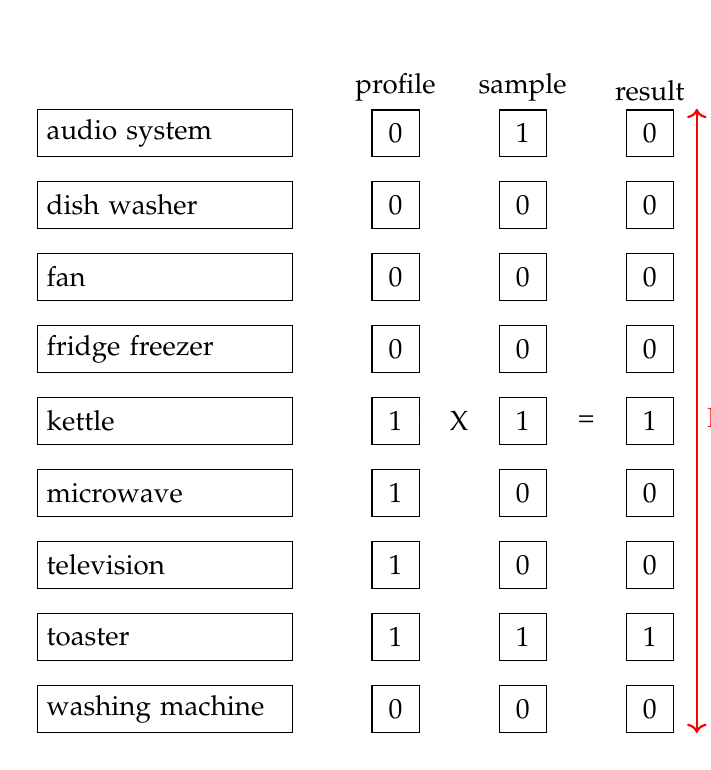
\begin{tikzpicture}
      \matrix [row sep=3mm, column sep=1cm,nodes={minimum size=6mm, draw, rectangle}]
      {
      \node[text width=3cm,white] {margin};\\ 
      \node[text width=3cm] {audio system}; &  \node (t1){0}; & \node  (t2){1}; & \node (s1){0};\\
      \node[text width=3cm] {dish washer}; &   \node     {0}; & \node     {0}; & \node     {0};\\
      \node[text width=3cm] {fan}; &           \node     {0}; & \node     {0}; & \node     {0};\\
      \node[text width=3cm] {fridge freezer}; &\node     {0}; & \node     {0}; & \node     {0};\\
      \node[text width=3cm] {kettle}; &        \node (a) {1}; & \node (b) {1}; & \node (c) {1};\\
      \node[text width=3cm] {microwave}; &     \node     {1}; & \node     {0}; & \node     {0};\\
      \node[text width=3cm] {television}; &    \node     {1}; & \node     {0}; & \node     {0};\\
      \node[text width=3cm] {toaster}; &       \node     {1}; & \node     {1}; & \node     {1};\\
      \node[text width=3cm] {washing machine}; &\node    {0}; & \node     {0}; & \node (s2){0};\\
      };
      \draw [<->,white] (a.east) -- (b.west) node[black] [midway] {X};
      \draw [<->,white] (b.east) -- (c.west) node[black] [midway] {=};
    
      \begin{scope}[transform canvas={yshift=0.8em}]
      \draw [-] (t1.west) -- (t1.east)node[black] [above,midway] {profile};
      \end{scope}  
    
      \begin{scope}[transform canvas={yshift=0.8em}]
      \draw [-] (t2.west) -- (t2.east)node[black] [above,midway] {sample};
      \end{scope}
    
      \begin{scope}[transform canvas={yshift=0.8em}]
      \draw [-] (s1.west) -- (s1.east)node[black] [above,midway] {result};
      \end{scope}
    
      \begin{scope}[transform canvas={xshift=1.7em}]
       \draw [<->,red,thick] (s1.north) -- (s2.south) node [right,midway] {IF SUM >= 2 not an anomaly};
      \end{scope}
    \end{tikzpicture}
    \caption{The evaluation of the test sample compared to the adjacent column from the matrix. An example is for a fifth bucket or fifth row from the matrix.}
    
\end{figure}

% \begin{figure}[H]
%     \centering
%     \caption{Process of evaluating an anomaly}
%     \includegraphics[width=1\linewidth]{../Figures/EC/EC_anom_dect.png}
%     \label{fig:anom_detct}
%     \caption{The evaluation of new bucket compared to matrix. An example is for a fifth bucket or fifth row from the matrix.}
    
% \end{figure}

This process is done for all samples, where we count normal and anomalous samples for each bucket.
The important thing to note here is that we are evaluating the samples from train data, from which the profile was built.

\begin{figure}[H]
    \centering
    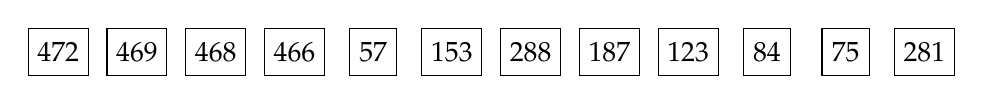
\begin{tikzpicture}
        \coordinate (s) at (0,0);
        \foreach \num in {472, 469, 468, 466, 57, 153, 288, 187, 123, 84, 75, 281}{
        \node[minimum size=6mm, draw, rectangle] at (s) {\num};
        \coordinate (s) at ($(s) + (1,0)$);
        }
    \end{tikzpicture}
    \caption{Aggregated anomalies for each bucket}
    \label{arr:agg_anom}
\end{figure}

\begin{figure}[H]
    \centering
    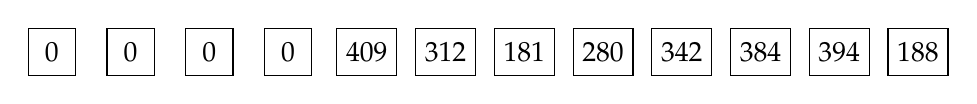
\begin{tikzpicture}
        \coordinate (s) at (0,0);
        \foreach \num in {0, 0, 0, 0, 409, 312, 181, 280, 342, 384, 394, 188}{
        \node[minimum size=6mm, draw, rectangle] at (s) {\num};
        \coordinate (s) at ($(s) + (1,0)$);
        }
    \end{tikzpicture}
    \caption{Aggregated normal samples for each bucket}
    \label{arr:agg_norm}
\end{figure}

\subsubsection{Step Five}

The next step is to combine these two arrays so that we calculate the percentage of anomalous samples 
for each bucket with an equation. 

\begin{equation}
    \frac{N_{anom}}{N_{anom}+N_{norm}}
    \label{eq:ratio}
\end{equation}

Where $N_{anom}$ is a number of anomalous samples and $N_{norm}$ is a number of normal samples.


We can modify Equation \ref{eq:ratio} so that it measures a number of normal samples out of the total samples. 
The result is the Equation \ref{eq:routine}
In other words, we are measuring the strength of a routine that the user maintains in each bucket.

\begin{equation}
    R_{outine}= \frac{N_{norm}}{N_{anom}+N_{norm}}
    \label{eq:routine}
\end{equation}

Using Equation \ref{eq:routine}, we can populate the array in Figure \ref{arr:anom_ratio}.

\begin{figure}[H]
    \centering
    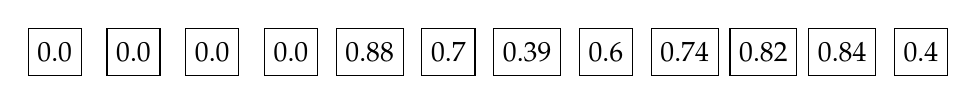
\begin{tikzpicture}
        \coordinate (s) at (0,0);
        \foreach \num in {0.0, 0.0, 0.0, 0.0, 0.88, 0.7, 0.39, 0.6, 0.74, 0.82, 0.84, 0.4}{
        \node[minimum size=6mm, draw, rectangle] at (s) {\num};
        \coordinate (s) at ($(s) + (1,0)$);
        }
    \end{tikzpicture}
    \caption{Aggregated anomalies for each bucket}
    \label{arr:anom_ratio}
\end{figure}

In other words, the array in Figure \ref{arr:anom_ratio} indicates the persistence of the user's routine in each bucket or part of the day.
The higher the metric, the stronger the routine.
Since routines are detected based on appliance usage, they cannot be detected during the night.

It is possible to see that the routine is quite high during the morning and evening hours.
The anomaly detection algorithm will perform best when the metric is high.
A notable characteristic of the elderly is that their routine is typically high even during the day.

Another thing to do is to ignore the parts of the day when the user has no detectable routine.
This is accomplished by using the array in Figure \ref{arr:anom_ratio} and setting a threshold of 0.7.

A threshold of 0.5 would imply that we could detect false positive anomalies every other day.
By setting the rate to 0.7, this is reduced to every third day.
Compromises must be made here; the lower the threshold, the more accurate the algorithm will be.
This also implies that it will be less sensitive.
In our case, there is not much harm in false positive detections, as the caregiver can call the elder to check if everything is okay.

\begin{figure}[H]
    \centering
    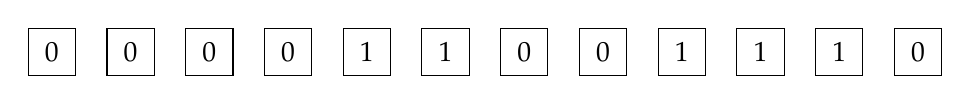
\begin{tikzpicture}
        \coordinate (s) at (0,0);
        \foreach \num in {0, 0, 0, 0, 1, 1, 0, 0, 1, 1, 1, 0}{
        %\foreach \num in {1.0, 1.0, 1.0, 1.0, 0.12, 0.3, 0.61, 0.4, 0.26, 0.18, 0.16, 0.6}{
        \node[minimum size=6mm, draw, rectangle] at (s) {\num};
        \coordinate (s) at ($(s) + (1,0)$);
        }
    \end{tikzpicture}
    \caption{Using the above-mentioned threshold a new mask is made, to check only buckets with high routine.}
    \label{arr:anom_ratio_mask}
\end{figure}

\subsubsection{Step Six}

The last step is to repeat Steps 4 and 5 with the test data.
When using the test data, we skip the buckets with low routine rates by using the mask from Figure \ref{arr:anom_ratio_mask}.
Since the profile has never seen the data being used, this should give us a good representation of actual performance in a real-world scenario.

\subsection{The metric - routine rate}

Due to the lack of ground truth data on actual accidents, it is hard to determine the exact accuracy of this algorithm. Every anomaly detected is not necessarily an actual accident, it could be that the user decided to lie in bed a bit longer, or decided to go to bed early in the evening.
One metric that we can use to determine how well the algorithm functions is the routine rate metric \ref{arr:anom_ratio}.
The reason behind this is that if the routine rate is high, it means that it will be easier to detect the actual anomaly.

\begin{itemize}
	\item A routine rate of 0 would mean that for that bucket, the household has no routine at all.
    \item A routine rate of 0.5 would mean that the routine is broken every second day.
    \item A routine rate of 0.8 would mean that the routine is broken on average every fifth day.
    \item A routine rate of 1 would mean that this household has a routine that is never broken. 
\end{itemize}

An example of when a user's routine rate is close to 1: When a true anomaly occurs such as a fall, the dweller, though he had maintained the same strong routine for the past year, would not be able to continue it, and the algorithm will be quite sure that this is an actual anomaly.
Therefore, the lower the routine rate, the less sure we are that an actual anomaly such as a fall occurred.
This is a good alternative measurement, which tells us how well this algorithm will perform. 
Since sometimes it is easier to read when results are presented as percentages, we will sometimes present them in this way.
 
\section{Results} 

Results were obtained for 3 datasets. 
The REDD and iAWE datasets were not used, since they were too small. 
They contained less than a month of data. 

\subsection{The Routine Rate Over a Period of Time}

In the following sections, we will present how the metric changes over given periods of time.
This will enable us to see the patterns that this metric helps reveal. 
Since we have more than a year of training data, this will allow us to observe how the metric changes over years.
This allows us to see how the routine changes over the year. 
We cannot use testing data in this case, as there is not enough of it.

\subsubsection{The Routine Rate Through the Week} \label{sssec:ratio_week}

As the behavior of the dweller changes, so does the accuracy of the algorithm. 
One observation that was made was that the routine was higher during the week than during the weekends,
as can be seen in Figure \ref{fig:ec_week} below. 
The only exception is Figure \ref{fig:ec_b5week}, which shows that the observation does not hold for all houses. 

\begin{figure}[H]
	\begin{subfigure}{.5\textwidth}
		% \centering
		\caption{Building 2}
		\includegraphics[width=1\linewidth]{../Figures/EC/b2week.pdf}
		\label{fig:ec_b2week}
	\end{subfigure}%
	~ 
	\begin{subfigure}{.5\textwidth}
		% \centering
		\caption{Building 19}
		\includegraphics[width=1\linewidth]{../Figures/EC/b19week.pdf}
		\label{fig:ec_b19week}
	\end{subfigure}%
    \bigskip

    \begin{subfigure}{.5\textwidth}
		% \centering
		\caption{Building 18}
		\includegraphics[width=1\linewidth]{../Figures/EC/b18week.pdf}
		\label{fig:ec_b18week}
	\end{subfigure}%
    ~ 
    \begin{subfigure}{.5\textwidth}
		% \centering
		\caption{Building 5}
		\includegraphics[width=1\linewidth]{../Figures/EC/b5week.pdf}
		\label{fig:ec_b5week}
	\end{subfigure}%
	\caption{Routine rate through the week (train data)}
    \label{fig:ec_week}
\end{figure}

Since we are dealing with the elderly, they have a consistent routine, and it does not vary significantly during the weekends.
Usually, assisted living systems are put in place because elders are alone in the dwelling.
Taking all of this into account, we could assume that the routine of the elderly remains the same throughout the week and simply ignore the weekends.
This should yield more relevant results.

\subsubsection{Routine Rate Through a Year}

The rate at which the routine is practiced also changes over a year.
While on average the routine rate is higher during the winter, spring, and fall, it is lower during the summer, due to vacations.
This can be seen in Figure \ref{fig:ec_year} below.
It is possible to observe dips in the routine.
In some cases, these dips occur in the summer and others in the springtime.
Without metadata, we cannot know for sure what was the event behind these dips.
There is a high chance that most of them are due to vacations or other events where one or more dwellers are away from home for extended periods of time.

\begin{figure}[H]
	\begin{subfigure}{.5\textwidth}
		% \centering
		\caption{Building 2}
		\includegraphics[width=1\linewidth]{../Figures/EC/b2year.pdf}
		\label{fig:ec_b2year}
	\end{subfigure}%
	~ 
	\begin{subfigure}{.5\textwidth}
		% \centering
		\caption{Building 19}
		\includegraphics[width=1\linewidth]{../Figures/EC/b19year.pdf}
		\label{fig:ec_b19year}
	\end{subfigure}%
    \bigskip

    \begin{subfigure}{.5\textwidth}
		% \centering
		\caption{Building 18}
		\includegraphics[width=1\linewidth]{../Figures/EC/b18year.pdf}
		\label{fig:ec_b18year}
	\end{subfigure}%
    ~ 
    \begin{subfigure}{.5\textwidth}
		% \centering
		\caption{Building 5}
		\includegraphics[width=1\linewidth]{../Figures/EC/b5year.pdf}
		\label{fig:ec_b5year}
	\end{subfigure}%
	
	\caption{Routine through the year (train data)}
    \label{fig:ec_year}
\end{figure}

\subsubsection{Effectiveness of Anomaly Detection Through the Day}

The following subsection will show how the effectiveness of anomaly detection changes throughout the day.

One thing to keep in mind is that this algorithm can detect anomalies only when
the routine is high, and when more than two appliances are used in given buckets.

Figure \ref{fig:ignored_buckets_22} shows which buckets are most commonly used for the detection of an anomaly.
The figure includes averaged values from all buildings and datasets.
In other words, the figure presents the strength of the average routine throughout the day.

This means that the higher the routine, the higher the chance that this bucket will be used for anomaly detection.
During the night, it is possible to see that the average routine rate is quite high.
This can be seen in Figure \ref{fig:ignored_buckets_22},
this is because most users are routinely sleeping during this period.
As we can see in Figure \ref{fig:ignored_buckets_22},
a high routine rate does not necessarily mean the buckets are useful.

\begin{figure}[H]
	\begin{subfigure}{.5\textwidth}
        \caption{Effectivity of anomaly detection through the day}
        \includegraphics[width=1\textwidth]{Figures/EC/ignored_buckets_dist.pdf}
        \label{fig:ignored_buckets_22}
    \end{subfigure}
    ~
    \begin{subfigure}{.5\textwidth}
        \caption{Actual effectiveness of anomaly detection through the day}
        \includegraphics[width=1\textwidth]{Figures/EC/all_ignored_buckets_dist_incl_act.pdf}
        \label{fig:ignored_buckets_act}
    \end{subfigure}
\end{figure}

To find the usable buckets, an additional filter must be applied.
The rule is that at least two appliances must be commonly used in each bucket. 
After applying this rule, the following Figure emerges \ref{fig:ignored_buckets_act}.

Figure \ref{fig:ignored_buckets_act} shows that there are two peaks:
one in the morning and a wider one in the evening.

This means that, on average, the algorithm would perform best in the morning and evening because the average person is at school or work during noon. 
Elderly individuals, who are usually at home at noon, could extend the effective detection window.

\subsubsection{The Anomaly Detection During the Night}

We have observed that anomalies can be detected throughout the day,
but are hard to detect during the night, since appliances are typically off.

In our current state, an anomaly occurs when something that should operate does not.
When the user is sleeping, an anomaly occurs when something that shouldn't operate does. 
To implement this additional rule, we would have to build two models:
one that operates during the day, and another that operates when the user is asleep.

To obtain information about the user's sleep schedule, we could either request a schedule from the user or extract it based on the usage pattern of appliances.
We can detect when most of the appliances are inactive and build a sleep profile based on this information.

Using the sleep schedule, it is possible to switch between the two operating modes. 
This new implementation would further extend the time windows within which we can detect anomalies and thus further improve users' safety.

The main issue is not the detection itself but efficiently determining
when the user is asleep. 

The examples above serve as a demonstration and a look into data and metrics. 
The examples shown were trained and evaluated on the same data. 
To show true performance, we will use test data to determine actual performance. 

\subsection{Per-Building Results}
\subsubsection{REFIT}

Results show that the method is, on average, \textbf{79.3} \% efficient for REFIT.  
In Figure \ref{fig:refit_res}, we can see that buildings 10 and 20 yield much worse results than the rest.
The overall routine pattern is very similar to Figure \ref{fig:tsne_euclidian} from the t-SNE chapter where we calculated the final Euclidean distance between samples of the t-SNE plot.
We will make a deeper analysis of this connection in the final Section \ref{sec:tsne_ec_corr} of this Chapter.

\begin{figure}[H]
	\begin{subfigure}{.5\textwidth}
        \caption{All buildings}
        \includegraphics[width=1\textwidth]{Figures/EC/refit_res.pdf}
        \label{fig:refit_res}
    \end{subfigure}
    ~
    \begin{subfigure}{.5\textwidth}
        \caption{Results for REFIT weekday only}
        \includegraphics[width=1\textwidth]{Figures/EC/refit_res_nw_1.pdf}
        \label{fig:refit_res_nw_1}
    \end{subfigure}
\end{figure}

As mentioned in Section \ref{sssec:ratio_week}, the average routine varies between weekdays and weekends.
The assumption was that the routine of elderly people does not change significantly throughout the week, therefore, results should be more relevant if we exclude the weekends.
Figure \ref{fig:refit_res_nw_1} shows that the result improved to \textbf{77.08} \%.
By removing the weekend data, the results improved by \textbf{1} \%.

\subsubsection{UK-DALE}

As mentioned in Section \ref{ssec:ds_eval}, the UK-DALE is not as big and clean of errors as the previous dataset, so the results could be less relevant.
The results in Figure \ref{fig:ukdale_res}, show that the average result is \textbf{74.48} \%.

\begin{figure}[H]
	\begin{subfigure}{.5\textwidth}
        \caption{Results for UK-DALE}
        \includegraphics[width=1\textwidth]{Figures/EC/ukdale_res.pdf}
        \label{fig:ukdale_res}
    \end{subfigure}
    ~
    \begin{subfigure}{.5\textwidth}
        \centering
        \caption{Results for UK-DALE omitting weekends}
        \includegraphics[width=1\textwidth]{Figures/EC/ukdale_nw_res.pdf}
        \label{fig:ukdale_res_nw}
    \end{subfigure}
\end{figure}


In this case, omitting the weekend data improves the routine slightly, increasing it to \textbf{74.51} \%.
There are many reasons behind this small improvement, one of which is, that the existing routine of these buildings does not change over the weekend.

\subsubsection{ECO}

ECO is of similar quality as UK-DALE when considering the number of buildings and the length of data, as can be seen in Section \ref{ssec:ds_eval}.
The results in Figure \ref{fig:eco_res} show that this dataset has the highest average routine rate of \textbf{83.80} \%.
As before, we can exclude the weekend data, which can be seen in Figure \ref{fig:eco_res_nw}. This brings the result up to \textbf{84.09} \%.

\begin{figure}[H]
	\begin{subfigure}{.5\textwidth}
        \caption{Results for ECO}
        \includegraphics[width=1\textwidth]{Figures/EC/eco_res.pdf}
        \label{fig:eco_res}
    \end{subfigure}
    ~ 
    \begin{subfigure}{.5\textwidth}
        \caption{Results for ECO omitting weekends}
        \includegraphics[width=1\textwidth]{Figures/EC/eco_res_nw_1.pdf}
        \label{fig:eco_res_nw}
    \end{subfigure}
\end{figure}


\subsection{Combined Results}

After combining results from all 26 buildings, Table \ref{tab:ec_res_weekend} can be populated.
It shows that the algorithm is \textbf{79.43} \% efficient at detecting true anomalies. 
On average, the algorithm would label \textbf{20.5} \% of samples as false positives, 
in other words, every fifth sample could be a false positive. 

\begin{table}[htbp]
    \centering
    \caption{Combined percentage [\%] of routine rate for 26 buildings}
    \label{tab:ec_res_weekend}
    \begin{tabular}{lcc}
        \hline
        \textbf{including weekend data} & \textbf{test} & \textbf{train} \\
        \hline
        \textbf{mean} & 79.43 & 84.55 \\
        \textbf{median} & 82.58 & 84.40 \\
        \textbf{standard deviation} & 14.62 & 9.05 \\
        \hline
        \end{tabular}
\end{table}

To understand the results a bit better, Figure \ref{ec:ec_histogram} presents the distribution of the samples.
It is possible to observe that the distribution is not normal as there is no bell-shaped pattern.
Such a distribution makes it hard to statistically analyze the results and makes it difficult to draw meaningful conclusions.
However, this issue can be addressed by visually analyzing and interpreting the data.
In this case, it is possible to see that a large portion (74 \%) of the samples fall in the interval above the mean, more specifically above the 80 \% routine rate.
This observation is important, as it adds another dimension to our understanding of the results.


\begin{figure}[H]
    \centering
    \caption{Histogram of results overlayed with a probability density function}
    \includegraphics[width=0.8\textwidth]{Figures/EC/ec_histogram.pdf}
    \label{fig:ec_histogram}
\end{figure}

If we assume that the average building in our dataset has altered routine during the weekend as can be seen in Figure \ref{fig:ec_week},
and assume that the average elder has roughly the same routine throughout the week, we can remove the weekend data
to obtain more relevant results.
Table \ref{tab:ec_res_no_weekend} shows the results after removing the weekend data.
We can observe that the mean test routine is \textbf{80.42} \%, which is slightly higher compared to the results from the previous Table \ref{tab:ec_res_weekend}.

\begin{table}[htbp]
    \centering
    \caption{Combined percentage [\%] of routine rate for 26 buildings not including weekend data}
    \label{tab:ec_res_no_weekend}
    \begin{tabular}{lcc}
        \hline
        \textbf{not-including weekend data} & \textbf{test} & \textbf{train} \\
        \hline
        \textbf{mean} & 80.42 & 85.88 \\
        \textbf{median} & 84.15 & 86.35 \\
        \textbf{standad deviation} & 15.58 & 8.25 \\
        \hline
        \end{tabular}
\end{table}

The last rows in Tables \ref{tab:ec_res_no_weekend} and \ref{tab:ec_res_weekend} show the standard deviation of our measurements,
which is 14.62 \% for weekend data and 15.58 \% for data that does not include weekends.
Even though the standard deviation is lower when excluding weekend data for the train data, it is higher for the test data, which was unexpected.

The reason can be seen in Figures \ref{fig:ec_histogram} and \ref{fig:ec_histogram_week_only},
where we have already observed the non-normal distribution, and mentioned that statistical methods should be analyzed with caution.

Visual analysis of Figure \ref{fig:ec_histogram_week_only} reveals that the general distribution did not change compared to Figure \ref{fig:ec_histogram}.
However, there are fewer samples above the 80 \% line and fewer samples with very low routine.
This could mean that not including weekend data may improve the overall score by aiding the worst performers, but it may also lower the score of the best performers.

\begin{figure}[H]
    \centering
    \caption{Histogram of results not including weekend data overlayed with a probability density function}
    \includegraphics[width=0.8\textwidth]{Figures/EC/ec_histogram_week_only.pdf}
    \label{fig:ec_histogram_week_only}
\end{figure}


When comparing the differences between the train and test data, it can be clearly observed that the train data performed better. 
The difference in performance can be attributed to the changed user behavior after the model was trained. 
It would be beneficial if we managed to update the model over time to include the small changes in users' routines. 
This will be addressed in the next section \ref{sec:iter_learning_system}.

\section{Discussion}

The main goal of our system is to detect anomalies when they occur.
The nature of this system is that there is more harm done if we do not detect an anomaly than if we detect a few false positives.
On the other hand, too many false positives could lead to caregivers ignoring detections altogether.
In this regard, we must find a balance between the two.
A false positive once a week is a good balance, especially since the caregiver is only a phone call away from checking the status of the patient.
Since the validation is so simple, we can claim that the performance of the system is adequate to be used in a real-world setting.

When analyzing these results, one important to keep in mind is,
that we do not have metadata available to know what kind of socio-economic status dwellers have.
Socio-economic status encompasses attributes such as age, income, number of children, geolocation, etc.
They may also encompass the age of the building, type of insulation, number of dwellers in the buildings, etc.
Since datasets do not provide them, it is hard to make any other conclusions other than the algorithm works well on an average building.

We know that the reason for installing such a system is that the user is left alone.
We can assume that on average there is more than one dweller living in the buildings we tested on.
Since this system would usually be used by a single dweller,
this would be in favor of our algorithm, as it would be easier to extract the routine.

One other thing that would be in our favor is, that the average person spends less time at home than an elderly person. 
If we take a look at the results, it is possible to see that, the average home has a low routine during the noon. 
This is because the average person is not at home during noon, which can be observed in Figure \ref{fig:ignored_buckets_22}.
Since the elderly are usually home at that time, this would increase the time windows where we can detect the accident.

We could also assume that the older the dweller, the higher the routine. 
The nature of the elderly is that they are more conservative when it comes to changes, and prefer to stick to their routine.
Since the algorithm works better when usage is periodic, this would also be in our favor. 
Taking all of these assumptions into account, there is a possibility that this algorithm would work better on the elderly due to their nature.
Since the results on the average building are promising a real-world setting test study should be performed. 
This would also prove our assumption that this algorithm works better on the elderly.

\section{Iterative Learning System}
\label{sec:iter_learning_system}
In the case of the practical use of this algorithm, it is important that the system is put online as fast as possible and that it improves over time.
This can be achieved with the implementation of iterative learning.
The algorithm will build an LP based on the first month of data.
Using this LP, the system can be immediately put online.
At the end of the month, it can use this data to improve the model, which can then be repeated indefinitely.

\subsection{Methodology}
The tools, metrics, and other methodologies are the same as in a normal learning system.
The only change that was made was on the data preparation side.

\subsubsection{Data Preparation}
For this evaluation, only REFIT (\cite{REFIT}) data was used.
As it can be seen in Figure \ref{fig:refit_timeline},
Refit buildings have long and relatively similar timelines
compared to other datasets.

In Figure \ref{fig:dyn_data_1}, it is possible to see
how the amount of training and testing data changes over 16 months.

\begin{figure}[H]
	\centering
	\caption{Data for building 1 over 16 months}
	\includegraphics[]{Figures/EC/DYN/tst_tr_b1.pdf}
	\label{fig:dyn_data_1}
\end{figure}

We can also plot how the amount of data changes for all buildings.
This can be seen in Figure \ref{fig:data_used_for_training}.

\begin{figure}[H]
	\begin{subfigure}{.5\textwidth}
        \caption{Data used for training}
        \includegraphics[width=1\textwidth]{Figures/EC/DYN/data_used_for_training_all.pdf}
        \label{fig:data_used_for_training}
    \end{subfigure}
    ~
    \begin{subfigure}{.5\textwidth}
        \caption{Data used for training, with removed buildings}
        \includegraphics[width=1\textwidth]{Figures/EC/DYN/data_used_for_training_removed_short.pdf}
        \label{fig:data_used_for_training_removed}
    \end{subfigure}
\end{figure}

To analyze the results, at least 1 year of usable data should be available.
Figure \ref{fig:data_used_for_training_removed} shows only buildings containing at least one year of data.
Similarly, we can check how test data changes over the months.
In this case, data is not being aggregated, but only one month of it is used at a time.
Figure \ref{fig:data_used_for_testing} shows that after one year,
the amount of data used for training starts to decline.
To get more accurate results, we will only observe the performance using one year of data.

\begin{figure}[H]
	\centering
	\caption{Data used for training, with removed buildings}
	\includegraphics[]{Figures/EC/DYN/data_used_for_testing.pdf}
	\label{fig:data_used_for_testing}
\end{figure}

\subsection{Results}

To show the effect of training data on the metric, Figure \ref{fig:efect_of_data_on_metric} is presented.
Figure \ref{fig:efect_of_data_on_metric} contains 12 months of data for each building.

\begin{figure}[H]
	\centering
	\caption{Effect of new data on metric}
	\includegraphics[]{Figures/EC/DYN/efect_of_data_on_metric.pdf}
	\label{fig:efect_of_data_on_metric}
\end{figure}

Figure \ref{fig:efect_of_data_on_metric} shows, that in most cases, results converge towards \textbf{80} \%. 
In some cases, the results are good from the beginning, but sooner or later the routine rate will dip. 
With more data, these dips become smaller and less frequent. 
If the behavior in the household radically changes, it can still lead to a dip.

\begin{figure}[H]
	\centering
	\caption{Metric over 12 months}
	\includegraphics[]{Figures/EC/DYN/1_year_of_iterative_learning_avg.pdf}
	\label{fig:1_year_of_iterative_learning_avg}
\end{figure}

Figure \ref{fig:1_year_of_iterative_learning_avg} shows how the same data can also be presented so that it shows how the metric changes over a year.
The same as in the previous Figure \ref{fig:efect_of_data_on_metric} we can observe the dips getting less frequent and smaller. 
Here we can also observe the average line. 
The average value seems to be on average at around \textbf{80 - 85} \%,

\subsection{Discussion}

It is hard to compare these results from iterative learning to the ones from non-iterative learning.
Even though the same data was used, different sections of it were used.

Let us consider the last point in Figure \ref{fig:1_year_of_iterative_learning_avg}, where the average is at the 85 \% mark, as an example.
Here, the amount of training data is different since we limited it to one year.
The training set is also different as only the last month was used, not 20 \%.
There are many differences between the train and test sets, so we cannot compare them.
The results do prove that the method works, and the true performance is around the expected 80 \%.

By increasing the amount of data, the algorithm becomes more stable.
In some cases, where users' behavior does not change, the algorithm could work from the first month onward.
In other cases, where behavior is more dynamic, the algorithm needs a month or two to stabilize.

It is important to note that the longer the observation, the higher the chance there is that the routine of the user will change.
When such changes do occur, the algorithms must have methods in place that enable them to adjust to the new routine.
The simplest approach would be to use weights that put more attention on more recent data and less attention on older data.

Future research in this area offers many open opportunities to improve the current approach.
For more accurate results, a method could be used where several synthetic anomalies are modeled and incorporated into existing data.
Additionally, the system could be set up in a real-world setting where elderly people live on their own.
Real anomalies would allow us to fully evaluate the system.
As mentioned, similar approaches already exist, so it would be essential to compare the accuracy of our method with other publications.
Additionally, we could compare our method to a more invasive method where the user wears a sensor such as a smart bracelet.

\section{Correlation Between t-SNE Plot Euclidean Distance and Routine Rate}
\label{sec:tsne_ec_corr}

In Section \ref{ssec:tsne_euclidian_distance}, we first observed the presence of periodic behavior in the formed t-SNE clusters.
We speculated that the scattering of LP clusters could be correlated to a routine; the smaller the scattering, the better the routine.
We calculated the scattering using Euclidean distance, which is the same metric used as a cost function in t-SNE.

Figure \ref{fig:tsne_euclidian2} was already presented in Section \ref{ssec:tsne_euclidian_distance},
but it makes sense to reuse it here in this context.
As mentioned, this Figure shows the Euclidean distance between samples for per-building LPs for every building.

\begin{figure}[H]
	\centering
	\caption{Euclidean distance of samples for every building using normalized LPs}
	\includegraphics[]{Figures/EC/CORR_TSNE/tnse_euclidian.pdf}
	\label{fig:tsne_euclidian2}
\end{figure}

To reveal the connection between the two, we plotted both on the same Figure \ref{fig:tsne_comparison}, where the routine rate is reused from results Figure \ref{fig:refit_res}.

\begin{figure}[H]
	\centering
	\caption{Plot of results from REFIT and t-SNE Euclidean distance }
	\includegraphics[]{Figures/EC/CORR_TSNE/TSNE_EC_comparison.pdf}
	\label{fig:tsne_comparison}
\end{figure}

Figure \ref{fig:tsne_norm} shows the same data as the Figure above, but it's normalized using a min-max scaler.
Additionally, we have inverted the values of Euclidean distance, since values seem to be inversely correlated.
Looking at the Figure it is clear that there is some similarity between the two columns,
especially for the best and worst-performing buildings.

\begin{figure}[H]
	\centering
	\caption{Normalized values}
	\includegraphics[]{Figures/EC/CORR_TSNE/TSNE_EC_norm.pdf}
	\label{fig:tsne_norm}
\end{figure}

To further prove the similarity, we have used the methodological approaches for calculating similarity that we explained in Section \ref{ssec:lp_similarity}.
The results can be observed in Table \ref{tab:similarity_results}.
First, we calculated cosine similarity using Equation \ref{eq:cosine_similarity}, which yielded a cosine similarity of \textbf{0.94} for the data seen in the second Figure \ref{fig:tsne_comparison} and \textbf{0.86} for the data seen in the third Figure \ref{fig:tsne_norm}.
Second, we calculated Pearson's correlation coefficient using Equation \ref{eq:pearson_correlation}, which yielded a result of \textbf{-0.76} for the data seen in the second Figure \ref{fig:tsne_comparison} and \textbf{0.76} for the data seen in the third Figure \ref{fig:tsne_norm}.
These values present that there is a connection between the t-SNE plot and the routine of the households.

\begin{table}[ht]
    \centering
    \caption{Similarity and correlation results}
    \label{tab:similarity_results}
    \begin{tabular}{@{}lcc@{}}
    \toprule
    \textbf{Method} & \textbf{Figure \ref{fig:tsne_comparison}} & \textbf{Figure \ref{fig:tsne_norm}} \\ \midrule
    Cosine similarity & 0.94 & 0.86 \\
    Pearson's correlation coefficient & -0.76 & 0.76 \\ \bottomrule
    \end{tabular}
\end{table}

When analyzing these results, we must keep in mind that the methodological approaches were very different for the two experiments.
In the case of t-SNE, we used normalized per-building LPs with very little preprocessing, whereas in the elderly care algorithm, we used per-building per-appliance LPs with extensive preprocessing to extract appliances that could help us detect the routine.
Another thing we must keep in mind is that elderly care enables us to detect anomalies on hourly intervals, whereas our t-SNE approach requires a minimum of a week of data to construct the LPs.
In this regard, t-SNE could be used to evaluate the routine rate of a household.

\subsection{Discussion}
This connection is an important demonstration that confirms our statements from Chapter \ref{chapter5} that the dispersion of samples in the t-SNE plot is related to routine.
This also means that we can rely on t-SNE to evaluate the routine of a household.
While it may not be as precise and fast as an elderly care algorithm, it is simple to use.
Apart from implementation being easily available, it uses per-building LPs, which can be built from most existing residential power meters.

This leads us to privacy issues, as almost all households use power meters for utility billing tracking. Before processing this data to build per-building LPs, the user should be informed and agree to the use of their data.
It should also be made clear that their data will be handled according to GDPR.

\section{Summary}

The results show that our approach can detect changes in routine and can improve over time.
Due to a lack of ground truth data, we were not able to measure the exact accuracy of the system,
but rather evaluate if the behavior of residents is sufficiently periodic.
Even the best algorithm would not be able to detect anomalies in a stochastic system.
With that, we also proved that such a system is sufficiently deterministic for such applications.

Furthermore, we have demonstrated the existence of a connection between the t-SNE plot and the routine obtained from the elderly care anomaly detection algorithm.
While t-SNE cannot be directly used in the setting of elderly care, as it's too slow, it could be used to determine if the routine of the household is strong enough before a more complex system is put in place.


% \chapter{Conclusion}
\label{chapter7}

In the introduction of Chapter \ref{chapter1}, it was said that the goal of the thesis will be achieved by contributing the following:

\begin{enumerate}
	\item Surveying the state-of-the-art LPs (Chapter \ref{chapter2})
	\item Development of multidimensional activation LPs (Chapter \ref{chapter4})
	\item Exploratory data analysis of activation LP's through t-SNE (Chapter \ref{chapter5})
	\item Propose a new anomaly detection method for elderly care (Chapter \ref{chapter6})
\end{enumerate}

With the first contribution, we have found new, previously unused ways of presenting the data.
This was achieved by building a detailed table of profiles such as we have seen in Chapter \ref{chapter2}.
This table presented the missing gaps, and which presentations were not used by the community.
We knew that not all unused profiles were useful, by using other publications we classified them based on their impact. 
We have selected the few with the highest impact and utilized used them in the following chapters.

Furthermore, we presented all the LPs in high detail. This was done so that the reader was able to understand what the LPs look like and what they present.
While doing so, we pointed out how some profiles could be used, and how we will use them to prove that they are useful. 

The third was contributed in Chapter \ref{chapter5}, where we have shown how data is connected in high-dimension space
using t-SNE for dimensionality reduction. Here we have shown how some buildings have more similar activation patterns than others.
Furthermore, we have shown which appliances are being used similarly. 
We have grouped the appliances into appliance groups and showed that appliances from different datasets are being used similarly, and how this method and groups can help us label unlabeled data. 
The formed clusters showed that a routine and persistent usage pattern does exist. This laid the groundwork for elderly care, where we have used this routine at the center of the algorithm.

The last was contributed in Chapter \ref{chapter6}, by building functioning elderly care assisted living system. 
The results proved that we successfully used one of the proposed LPs in a real-world scenario. 
The main goal was to efficiently extract the routine, and build a working system around it.
The results show that we have succeeded in doing so and that the algorithm is adequate to be used in the real world.
To further prepare the algorithm for the real world, we have implemented an iterative learning system.
The system could be put online a month after the installation of the system and continues to improve over time.
Furthermore, we have shown that a correlation between t-SNE euclidean distance and calculated routine rate does exist,
which proves our statement from Chapter \ref{chapter5} that formed clusters present routine.

We believe that our work has contributed new tools for understanding energy consumption and leveraging energy data as a passive sensor to detect anomalies in the consumption itself.
Energy efficiency and the independence and well-being of the elderly are just two use-cases we addressed.
There is still much more to learn about how and which LPs can be used to improve our lives.
While we have filled in a few gaps in the table of profiles, it is up to scientific community to fill in the rest.

% [We could go into larger details and use other dimensionality reduction algorithms for comparison, or even have more empirical proofs. 
% In the case of elderly care, we could use the results or algorithms of other publications to compare it to ours, or even compare it to the other intrusive methods. 
% This could all be done in greater detail.

% In the end, that was not the goal.
% The goal of the thesis was to prove that the proposed profiles can be efficiently utilized. 
% By doing that, we have achieved the main goal of the thesis,
% that was "to propose suitable consumption profiles for supporting residential building consumption optimization and elderly care management".
% With that, we can conclude the thesis with the following words:

% The ever-increasing amount of data is available to the scientific community.
% This data can be fully utilized if we find ways to efficiently extract the information that it is holding.
% The sole purpose of the LPs is to reveal patterns, contextual features and information itself in the vast sea of data.
% With the proposed LPs, we have hopefully contributed new tools that will help researchers to uncover the truths that the datasets hold. 
% While we have filled in a few gaps in the table of profiles, it is up to scientists community to fill in the rest.]

% %----------------------------------------------------------------------------------------
% %	THESIS CONTENT - APPENDICES
% %----------------------------------------------------------------------------------------

\appendix % Cue to tell LaTeX that the following "chapters" are Appendices

% % Include the appendices of the thesis as separate files from the Appendices folder
% % Uncomment the lines as you write the Appendices

% Appendix A

\chapter{The Source Code, High-Resolution Figures and Datasets} % Main appendix title

\label{AppendixA} % For referencing this appendix elsewhere, use \ref{AppendixA}

The following appendix contains mostly links that point to GitHub.
GitHub should be a valid repository for such projects, where links should persist indefinitely.
In case the links do eventually break, you can find the repository of thesis and demos under the username "jenkoj", under "msc" and "appliance-profiling".

\section{The source code}

The source code used in this chapter can be found in a GitHub repository: \\
\noindent \url{https://github.com/jenkoj/appliance-profiling} \\

\noindent Individual scripts can be found in the following Jupyter Notebooks: \\

\noindent The source code for generating the figures can be found at: \\
\noindent \url{https://github.com/jenkoj/appliance-profiling/blob/main/profilng_slices.ipynb} \\

\noindent The source code for t-SNE can be found at: \\
\noindent \url{https://github.com/jenkoj/appliance-profiling/blob/main/t_SNE.ipynb} \\

\noindent the source code for elderly care can be found at: \\
\noindent \url{https://github.com/jenkoj/appliance-profiling/blob/main/elderly_care_demo.ipynb} \\

\section{High resolution figures}

\noindent High-resolution figures can be found in the thesis repository \url{https://github.com/jenkoj/msc}. \\
\noindent More precisely in the "figures" subfolder \url{https://github.com/jenkoj/msc/tree/main/Figures}. \\

\section{Data and datasets}

\noindent We cannot share the data since it is not ours to share, but we can share the spreadsheet that points to each dataset.
\noindent The spreadsheet includes other datasets that could be used for the very same purpose.
\noindent The spreadsheet can be found here.  \\

\noindent \url{https://github.com/jenkoj/msc/blob/main/Appendices/datasets_and_sources.pdf} \\

\noindent An overview of the data in the datasets was made, and it can be seen in the following spreadsheet.  \\
\noindent \url{https://github.com/jenkoj/msc/blob/main/Appendices/dataset_overview.pdf} \\

\noindent The sliced hourly datasets can be found here. \\
\noindent \url{https://drive.google.com/drive/folders/1tIsG-bqxoJdbU1p8xa_LCTaKNSk_LylZ?usp=sharing} \\




% {mall\verb!\hypersetup{urlcolor=red}!}, or

% {\small\verb!\hypersetup{citecolor=green}!}, or

% {\small\verb!\hypersetup{allcolor=blue}!}.

% \noindent If you want to completely hide the links, you can use: 

% {\small\verb!\hypersetup{allcolors=.}!}, or even better: 

% {\small\verb!\hypersetup{hidelinks}!}.

% \noindent If you want to have obvious links in the PDF but not the printed text, use:

% {\small\verb!\hypersetup{colorlinks=false}!}.
% \s
% Appendix A

\chapter{Expanded General Table} % Main appendix title

\label{AppendixB} % For referencing this appendix elsewhere, use \ref{AppendixA}

\begin{table}[H]
    \caption{Expanded general table of load profiles}
    \label{tab:extended_general_map}
    \begin{tabular}{|c|c|c|c|c|c|}
    \hline
        &
        frequency &
        appliances &
        \begin{tabular}[c]{@{}l@{}}number of\\ activations\end{tabular} &
        \begin{tabular}[c]{@{}l@{}}power\\ (avg)\end{tabular} &
        \begin{tabular}[c]{@{}l@{}}operating\\ time\end{tabular} \\ \hline
    appliances                                                      &   & X & X & X  & X    \\ \hline
    \begin{tabular}[c]{@{}c@{}}number of\\ activations\end{tabular} & X & \multicolumn{1}{c|}{\begin{tabular}[c]{@{}c@{}} \citeyear*{per_appliance_per_building} \\ \citeyear*{UKDALE} \end{tabular}} & X & X  & X    \\ \hline
    \begin{tabular}[c]{@{}c@{}}power \\ (avg)\end{tabular}          & X & \citeyear*{appliance_avgpower} &   & X  & X    \\ \hline
    \begin{tabular}[c]{@{}c@{}}power \\ (array)\end{tabular}        & \citeyear*{UKDALE} & X & X & X  & X    \\ \hline
    \begin{tabular}[c]{@{}c@{}}power \\ (histogram)\end{tabular}    &   &   & X & X  & X    \\ \hline
    \begin{tabular}[c]{@{}c@{}}operating\\ time\end{tabular}        & X & \citeyear*{operating_time} & \multicolumn{1}{c|}{\begin{tabular}[c]{@{}c@{}} \citeyear*{NILMAD2019} \\ \citeyear*{NILMAD22019} \\ \citeyear*{NILMAD2021} \end{tabular}} &  \citeyear*{NILMAD2021} & X    \\ \hline
    time array                                                      & X & X & \multicolumn{1}{c|}{\begin{tabular}[c]{@{}c@{}} \citeyear*{per_appliance_per_building} \\ \citeyear*{UKDALE} \end{tabular}} &  \multicolumn{1}{c|}{\begin{tabular}[c]{@{}c@{}} \citeyear*{Chuan2014} \\ \citeyear*{Csoknyai2019} \\ \citeyear*{H0} \\ \citeyear*{KAVOUSIAN2013184} \\ \citeyear*{WALKER1985} \\ 	\citeyear*{GERBEC2005} \\ 	\citeyear*{Gao2018} \\ 	\citeyear*{Jeong2021}\\  	\citeyear*{Joana2012} \\ 	\citeyear*{DER_heatmap_profile}\\ 	\citeyear*{NILMAD2019}\\	\citeyear*{NILMAD22019} \\	\citeyear*{Issi2018} \\	\citeyear*{NILMAD2021}\\	\citeyear*{Castangia2021} \\	\citeyear*{occupancy2013} \\	\citeyear*{Chuan2014} \\ 	\citeyear*{CAPASSO1994} \\ 	\citeyear*{Park2019} \\	\citeyear*{UKDALE} \\	\citeyear*{Gao2018} \end{tabular}}    & \citeyear*{OperatingTime_timeofday} \\ \hline
    \end{tabular}
\end{table}

% The first profile is the one in the first row and the first column.
% It is a combination of frequency and appliances. 
% This would mean that we would have appliances on the x-axis and the number of occurrences o the y-axis.
% The only useful application for this profile is when presenting how many appliances of one type are in one dataset. 
% Other than that it has no use-cases and that is probably the reason why it is rarely used.

% The next possible combination is between a number of activations and appliances. 
% Here the explanation is relatively straightforward. The combination shows us how many times each appliance activities.

% The second presentation of data is a combination of power and number of activations. 
% In this case, we would construct a histogram of power values. 
% On the x-axis we would have power values on the y-Axis we would have a number of times this power value occurred, where we would have buckets of a certain size.
% Here we should not mix it up with the previous combination, since here we include the whole consumption and not only when turned on. 

% The combination in the second column and second row is between average power, an integer, and appliances. Again explanation is simple. We present the average consumption for each appliance in a household.

% The combination in the third column and second row, between average power and numbers of activations, is again less straightforward.
% It presents how many times it activated with a certain power.

% Here one feature is an output of the previous combination, a histogram of power. 
% It is possible to have a histogram of the histogram, but it is not practical. 
% This means we are looking at looking how many times did the occurrence occur. 
% Not all combinations, even though they are possible, are useful. 

% The combination in the second column and fifth row is again straightforward. 
% Plotting histograms for each appliance and then plotting them side by side.
% In this case, we present histograms in color, since we are working with 3 dimensions.

% In the case of combining the second column and sixth row, between appliances and operating time, we present how long each appliance operates.
% Here it could be either a number or even a time range presentation.
% When doing a combination between operating time and the number of activations we are plotting how many times did an appliance turn on for a certain amount of time

% In the case of a combination between operating time and power, we show how long did appliance operate with a certain power.

% Next case, in the third row and last column, a combination between time array and several activations we present when did appliance turn on certain amount of times. 

% We are coming to an end, and here we have the most commonly used case where we use time array and average power to present the data.

% In the final case, the combination shows us at which time do appliance operate for a certain amount of time 

% %\include{Appendices/AppendixC}

%----------------------------------------------------------------------------------------
%	BIBLIOGRAPHY
%----------------------------------------------------------------------------------------
\printbibliography[heading=bibintoc]
%#\bibliography{acm} 
%----------------------------------------------------------------------------------------

\end{document}  